%\documentclass[a4paper,11pt]{article}
\documentclass[a4paper,11pt]{article}
				
%packages will now follow
%Packages here is just for aestestics%%
\usepackage{lmodern}
\usepackage[T1]{fontenc}
%%%%%%%%%%
\usepackage[hmargin={25mm,25mm},vmargin={25mm,25mm}]{geometry}
\usepackage{amsmath,amsfonts,amsthm} %math package
\usepackage{breqn}  %math package
\numberwithin{equation}{section}
\usepackage{float}
\usepackage{graphicx, xcolor}
\usepackage[outdir=./Graphs/]{epstopdf}
%%%%%%%%%%%%%%%%
\usepackage{hyperref}
\usepackage{bigints}
\usepackage{enumerate}
\usepackage{parskip}
\usepackage{wrapfig}
\usepackage{lipsum}
\usepackage{lscape}
\usepackage{threeparttable}
\usepackage{longtable}
\usepackage{multirow}
\usepackage{caption,booktabs,array}
\usepackage{url}
\usepackage{xspace}
\usepackage{tabto}
\usepackage{pdflscape}
\usepackage{chngcntr}
\usepackage[bottom]{footmisc}
%\counterwithout{footnote}{chapter}
\usepackage[nottoc]{tocbibind}


%\usepackage{babel}

\setlength{\extrarowheight}{3pt}

\newcommand{\rowgroup}[1]{\hspace{-1em}#1}
\newcommand\cites[1]{\citeauthor{#1}'s\ (\citeyear{#1})}
\newcommand\citesall[1]{\citeauthor*{#1}'s\ (\citeyear{#1})}
\newcolumntype{P}[1]{>{\centering\arraybackslash}p{#1}}

\usepackage{tocloft}
\renewcommand{\cftfigfont}{Figure }
\renewcommand{\cfttabfont}{Table }
%\renewcommand{\bibname}{List of References}

\usepackage{fancyhdr}
\pagestyle{fancy}

\fancyhead[C]{}
\fancyhead[R]{}
\fancyhead[L]{}

\fancyfoot[C]{\thepage}
\fancyfoot[R]{}
\fancyfoot[L]{}

\renewcommand{\headrulewidth}{0pt}
\renewcommand{\footrulewidth}{0pt}

\usepackage{array}
\newcolumntype{x}[1]{>{\centering\arraybackslash\hspace{0pt}}p{#1}}

\usepackage{natbib}

\setlength{\parindent}{0cm}
\setlength{\parskip}{1.3ex plus 0.5ex minus 0.3ex}

\graphicspath{{Graphs/}}
\usepackage[font=small]{caption}

\title{\textsc{A medium-sized, open-economy, fiscal DSGE model of South Africa}\footnote{This paper represents and edited version of a chapter contained in an original PhD dissertation, entitled \textit{Essays on fiscal policy in South Africa}, completed at the University of Stellenbosch. Original copyright belongs to the University of Stellenbosch.}}

\author{

Johannes Hermanus Kemp\footnote{Stellenbosch University, Stellenbosch, South Africa; johannes.kemp@gmail.com}

\and

Hylton Hollander\footnote{Department of Economics, Stellenbosch University, Stellenbosch, South Africa; hylton@sun.ac.za} 

}


%-----------------------------------------------------------------------------------------------------------------------------

\begin{document}
	
%-----------------------------------------------------------------------------------------------------------------------------

\maketitle
	\thispagestyle{empty}
	\noindent\rule{16.5cm}{0.4pt}
	
	\begin{abstract}
		  \noindent Much of the research on fiscal multipliers has used reduced-form modelling approaches. While these models have been extended to include richer controls and innovative identification approaches, a question that often arises is whether shocks identified in these models capture the true structural shocks. An alternative, more theoretically way to identify shocks to government spending and taxes is through DSGE models. To that end, this paper estimates an open-economy DSGE model in the New Keynesian tradition, but with a more detailed fiscal block, to improve our understating of the impact of fiscal policy shocks on macroeconomic outcomes in the South African context. Policy simulations indicate that government spending and investment multipliers are generally positive, albeit smaller than one. Secondly, it is found that taxes are highly distortionary, with large negative multipliers for private consumption and investment. In contrast, the impact of tax shocks on output is ambiguous and depends on assumptions regarding the functional form of the different fiscal rules. Finally, simulations suggest that government consumption spending and, to a lesser extent, labour and consumption taxes are the most effective instruments for stabilising debt after a fiscal shock. 
	\end{abstract}
	
	\noindent\rule{16.5cm}{0.4pt}
	
	%\tableofcontents
	
%\vfill

\textbf{JEL Classification:} C32, E32, E62, H62, H63
	
\textbf{Keywords:} DSGE model; fiscal policy; fiscal multiplier; Bayesian inference 
	
\newpage
\pagenumbering{arabic}


\section{Introduction}
	
	Much of the research on fiscal multipliers has used reduced-form modelling approaches. While these models have been extended to include richer controls and innovative identification approaches in an effort to refine the analysis, a question that often arises is whether shocks identified in these reduced-form models, more often than not with minimal theoretical restrictions, capture the \textit{true} structural shocks. 
	
	An alternative, more theoretically way to identify shocks to government spending and taxes is through estimated dynamic stochastic general equilibrium (DSGE) models. Given their theoretical consistency and inherently forward-looking nature, DSGE models present a useful tool for policy analysis, and fiscal policy analysis in particular. The rational expectations paradigm embedded in the DSGE framework imply that agents' beliefs about which fiscal instruments are used to finance public debt play a crucial role in the determination of the equilibrium as well as the dynamic response of endogenous variables, including output. 
	
	In light of these considerations, an open-economy DSGE model in the New Keynesian tradition, but with a more detailed fiscal block as in \cite{coenen2013}, is estimated in an attempt to improve our understating of the size (and direction) of the impact of fiscal policy shocks on macroeconomic outcomes in the South African context. Apart from the now standard set of nominal rigidities, the model contains several features that make it suitable for fiscal policy analysis, namely non-Ricardian (or rule-of-thumb) consumers, utility-enhancing government spending, and distortionary taxes.
	
	Policy simulations based on the estimated model indicate that government spending and investment multipliers are generally positive, albeit smaller than one. Secondly, it is found that taxes are highly distortionary, with large negative multipliers for private consumption and investment. In contrast, the impact of tax shocks on output is ambiguous and depends on assumptions regarding the functional form of the different fiscal rules. Finally, an investigation into debt dynamics suggests that government consumption spending and, to a lesser extent, labour and consumption taxes are the most effective instruments for stabilising debt after a fiscal shock. 
	
	The rest of the paper proceeds as follows: Section \ref{lit_rev} provides a brief overview of the literature, while Section \ref{model_dsge} provides details on the DSGE model. Section \ref{estimation} provides details on the estimation procedure as well as estimation results. Section \ref{simulations} presents various simulation results, including fiscal multiplier analysis, and Section \ref{con_dsge} concludes with some final thoughts and ideas for further research.
	
	\section{Literature review} \label{lit_rev}
	
	As mentioned before, while the international literature is filled with studies into the effects of fiscal policy on macroeconomic outcomes, no consensus has been reached on the size (or sign) of government spending multipliers. 
	
	In one of the earliest studies on the impact of fiscal policy decisions using structural general equilibrium models, \cite{baxter1993} showed that in a simple real business cycle (RBC) model extended to include lumpsum taxes, an increase in government spending results in a negative wealth effect for households due to the associated increase in the discounted future value of taxes. This negative wealth effect, in turn, induces a positive labour supply response and an associated decrease in private consumption and a fall in real wages. New Keynesian models (which add both real and nominal frictions to the RBC framework), display the same wealth-effect that induces a positive labour supply response and a fall in private consumption, although in this context real wages might increase as a result of increased demand for labour \citep{forni2009}. 
	
	However, these theoretical correlations did not appear to match up with evidence from applied research. In order to reconcile the theoretical predictions with results from the empirical literature, recent studies in the DSGE literature has recognised the heterogeneity in consumer behaviour apparent in the data and moved away from the restrictive assumption of the representative, infinitely-lived, rational agent. \cite{mankiw} argued that models that contain both Ricardian and non-Ricardian agents (that do not have access to financial markets and, as such, cannot save or borrow to augment consumption expenditure) is better suited for fiscal policy analysis. The seminal contribution by \cite{gali} embedded rule-of-thumb (or non-Ricardian) agents in a standard monetary New Keynesian model. They found that the presence of these rule-of-thumb consumers, together with sticky prices and deficit financing, produces sizeable positive fiscal multipliers in the model economy.
	
	Subsequent literature embedded this idea of rule-of-thumb consumers in the class of models of \cite{smets2005,smets2007} and \cite{christiano2005}. These models incorporate many of the features that have been shown to be useful in accounting for different aspects of the variation in macroeconomic aggregates, such as sticky prices, sticky wages, investment adjustment costs, habit persistence, etc. These richer models were shown to match the data reasonably well and could be used to generate estimates of the quantitative importance of rule-of-thumb consumers. Seminal examples of efforts in that direction can be found in \cite{coenen2005}, \cite{erceg2006}, \cite{rabanal2006} and \cite{forni2009}. 
	
	In contrast to \cite{gali}, \cite{coenen2005} found that little evidence that government spending shocks crowd in consumption, mainly because the estimated share of rule-of-thumb consumers is relatively low for the Eurozone - the estimated share of non-Ricardian households across their sample is significantly smaller than the mean of the prior which was set equal 0.5 on the basis of micro-based estimates obtained for the pre-1990 period in the US. In contrast, \cite{erceg2006} found large, positive short-run fiscal multipliers associated with temporary increases in government spending. Similarly, \cite{rabanal2006} found that private consumption increases after a government spending shock when either non-separability in consumption-hours, non-Ricardian behaviour, or both, are introduced in the model.  
	
	Most of the early literature focused on lump-sum taxes and aggregate government spending. \cite{forni2009}, among others, extended the framework of \cite{christiano2005} and \cite{gali} by including a detailed fiscal block. On the revenue side, the authors considered different distortionary tax rates, embedded in simple policy rules. On the expenditure side, they considered government consumption excluding compensation for public employees (or government purchases of goods and services) and modelled public employment separately in order to gauge the differential impact of the different types of spending. They found that shocks to government purchases of goods and services and public sector compensation have small and temporary effects on macroeconomic aggregates, while shocks to transfers have a slightly larger and more permanent effect. The effects are more significant on the revenue side, with cuts in labour and consumption taxes inducing sizeable consumption and output responses, while reductions in capital taxes have a positive effect on private investment and total output in the medium run. 
	
	This highlights the importance of studying the underlying mix of government spending and tax decisions rather than just aggregate quantities. \cite{mountford} found substantial multipliers for the US that are comparable to those of \cite{blanchard2002}, but emphasized that tax cuts are more effective in stimulating demand than increases in government spending as the private consumption response to government spending increases is insignificant. In a similar vein, \cite{coenen2012} used a version of the European Central Bank's New Area-Wide Model extended to include a detailed specification of the fiscal sector and found that discretionary fiscal measures implemented during the GFC increased annualized quarterly real GDP growth by up to 1.6 percentage points. However, the authors noted that a detailed modelling of the fiscal sector and the incorporation of several fiscal time series were pivotal for the result. \cite{carvalho2011} further distinguished between private and public capital accumulation and provides a mechanism through which public capital augments factor productivity in the private sector. This provides an additional avenue through which fiscal policy decisions can impact on real macroeconomic outcomes. 
	
	An alternative approach that seeks to mimic the positive wage and consumption responses often found in the empirical literature entails the introduction of a different habit formation process on the part of consumers. \cite{ravn2010} developed a model of deep habits, which manages to produce positive consumption effects following a government spending impulse.\footnote{Deep habits imply that households form habits over sub-categories of consumption goods, such as cars and clothing, as opposed to aggregate consumption.}  \cite{christoffel2011} introduced a specific form of habit formation in the composite of consumption and leisure (as in \citealp{jaccard2010}) in order to study their model's ability to generate a realistic bond premium, but at the same time find significant fiscal multipliers. 
	
	A further aspect of the policy response to the GFC that received little attention initially but has gained prominence recently is the fact that monetary and fiscal policy reacted \textit{jointly} in an effort to stimulate demand. The interaction between monetary and fiscal policy is particularly important in an environment where governments the world over contemplate when and how to normalise policy. This interaction has important implications for the size of the fiscal multiplier. \cite{davig} estimated Markov-switching policy rules for the US and found that monetary and fiscal policies fluctuate between active and passive states and that shocks to government spending induces positive consumption responses under certain policy regimes. In a follow-up paper, \cite{leeper2015} found different sized multipliers for the US under different monetary-fiscal policy regimes. While output multipliers are comparable across regimes over the short-run, in the long run multipliers are much larger under the passive monetary/active fiscal policy regime than under active monetary/passive fiscal policy regime. Using a time varying parameter vector autoregression (TVP-VAR), \cite{jooste} found fiscal multipliers for South Africa that differ across time and between expansions and recessions. In fact, a common finding in the literature is that fiscal policy appears to be more effective during periods of economic downturn than during expansions (see \citealp{auerbach}; \citealp{baum2012}; \citealp{owyang2013}; \citealp{auerbach2014}; \citealp{canzoneri2015}, among others). 
	
	Other studies have also investigated the impact of fiscal decisions when monetary policy is at (or close to) the zero nominal interest rate bound. \cite{hall} found that in an economy with an output multiplier of just under one in normal times, the multiplier can rise to 1.7 at a zero nominal interest rate, while \cite{christiano2011} obtained an even stronger effect. Using a two-state Markov-switching framework, \cite{eggertsson2011} found that multipliers can be up to five times larger at the zero lower bound.
	
	Several extensions have sought to enrich the basic model specifications in order to more closely resemble actual economies. One such extension is the inclusion of a mechanism for fiscal foresight on the model economy. According to \cite{ramey2011b} and \cite{leeper2012}, models that do not explicitly account for foresight is misspecified and biased responses. As shown in \cite{jooste2017}, fiscal foresight eliminates the results of \cite{gali} in that a large share of rule-of-thumb consumers is not enough to generate positive co-movement between government spending and consumption. However, under certain calibrations, the inclusion of sticky wages still generates positive consumption responses and produces sizeable output multipliers. 
	
	The greater proportion of the literature on fiscal multipliers focus on closed economies in the vein of \cite{gali}. While some studies have investigated the impact of fiscal policy decisions within the context of an open economy (see \citealp{erceg2006}; \citealp{cavallo2007}; \citealp{ratto2007}; \citealp{levine2009}; \citealp{horvath2014}; \citealp{petros2019} for examples), this is much less prevalent. This aspect is particularly important in the context of the South Africa economy and given the assertion in the literature that fiscal multipliers are generally smaller in an open economy setting.
	
	Finally, despite the international interest in estimating the impact of fiscal shocks on macroeconomic outcomes, very little work has been done in the South African context. A notable exception is \cite{jooste} who investigated the impact of fiscal policy shocks using three models: a medium-scale, closed-economy DSGE model, a (open-economy) structural vector error correction model (SVECM), and a time varying parameter vector autoregression (TVP-VAR). The use of these non-standard models allows the authors to answer some of the important questions raised in the field pertaining to the weaknesses of standard VARs (mentioned above). The authors found that increases in government expenditure have a positive effect on GDP in the short run (albeit less than unity in some instances), but that the impact becomes negligible in the long run. Similar results hold for changes to tax policy.
	
	This paper adds to the burgeoning fiscal DSGE literature by extending the baseline closed-economy model to an open economy setting, while at the same time including a more detailed fiscal sector and estimating key parameters. 
	
	\section{The Model} \label{model_dsge}

	% % % % % % % % % % % % % % % % % % % % % % % % % HOUSEHOLDS % % % % % % % % % % % % % % % % % % % % % % % % % % % % % % % % % %
	
	The small open economy model structure closely follows that of \cite{adolfson2007} and \cite{christoffel2008}, while incorporating a more active role for fiscal policy along the lines of \cite{coenen2013}.\footnote{See \cite{steinbach2014} for an application of the \cite{adolfson2007} model to South Africa.}
	
	The basic open economy structure is relatively standard: Households consume both domestic and imported consumer goods, while optimizing agents can invest in domestic and foreign bonds. The optimizing households rent capital to firms and decide how much to invest each period, with changes to the rate of investment, as well as changes to the rate of capital utilisation, subject to adjustment costs. Each household supplies a differentiated labour service to firms, allowing them to set their wage in a \cite{calvo1983} manner. 
	
	The model contains three types of firms: domestic producers, importers and exporters. Domestic firms employ labour and capital in production. A differentiated good is produced by each type of firm. Prices are set following \cites{calvo1983} model, but with a variation that allows for the indexation to past inflation (following \cite{rabanal2006}).
	
	Finally, monetary policy follows a standard Taylor-type rule, while	the foreign economy is assumed to be exogenous.
	
	This basic specification is extended along the lines of \cite{coenen2013} to include a more active role for fiscal policy. The specification of the fiscal sector balances the need for a high degree of detail, which is essential for analysing the quantitative effects of fiscal policy innovations, and tractability, which allows for the identification of the relevant transmission mechanisms. Specifically, the model includes (i) non-Ricardian (or rule-of-thumb) consumers to facilitate a direct transmission mechanism for government transfers, (ii) government consumption that enters the households' utility function in a non-separable way, (iii) public capital which can either be a complement or substitute for private capital, (iv) time-varying distortionary taxes, and (v) a set of fiscal rules governing the endogenous response of fiscal variables.
	
	\subsection{Households}
	
	There is a continuum of households $h\in [ 0, 1 ]$. They derive utility from consuming a basket of domestic consumption goods, both private and public, while they exhibit disutility in supplying labour services.
	
	Following \cite{coenen2005}, \cite{gali}, \cite{jooste}, and \cite{coenen2013}, among others, the household sector is divided into two distinct groups. A share $i\in(\omega,1]$ of households - referred to as Ricardian households - invest, accumulate capital and have access to both foreign and domestic financial markets, and display the standard optimizing behaviour. The remaining share $j\in[0,\omega]$ of households - referred to as non-Ricardian households - do not trade in assets and simply consume their after-tax disposable income. Importantly, Ricardian households can smooth consumption intertemporally in response to shocks, whereas non-Ricardian simply consume their after-tax disposable income (\citealp{coenen2013}).
	
	Furthermore, it is assumed that valuable government consumption enters the households' utility function in a non-separable way. This feature has two important implications. First, under this specification, shocks to government consumption affect optimal private consumption decisions directly. This stands in contrast to the indirect wealth effect associated with separable government consumption. Second, the feature implies that it is theoretically possible to generate co-movements between private and government consumption, conditional on the estimated degree of complementarity.
	
	Formally, aggregate consumption $\tilde{C}_{h,t}$ of household $h$ is defined as a constant elasticity of substitution (CES) aggregate
	
	\begin{equation} \label{cons}
	\tilde{C}_{h,t}=\left(\alpha_G^{\frac{1}{\nu_G}}\left(C_{h,t}\right)^{\frac{\nu_G-1}{\nu_G}}+\left(1-\alpha_G\right)^{\frac{1}{\nu_G}}\left(G_t\right)^{\frac{\nu_G-1}{\nu_G}}\right)^{\frac{\nu_G}{\nu_G-1}}
	\end{equation} 
	
	where $C_{h,t}$ denotes the household's consumption of private goods and $G_t$ measures government consumption. $\alpha_G$ is a share parameter and $\nu_G$ measures the elasticity of substitution between private consumption and government consumption, with $\nu_G>0$. In particular, $\nu_G\rightarrow0$ implies that private and public consumption are perfect complements, $\nu_G\rightarrow\infty$ results in perfect substitutability, and the Cobb-Douglas case is obtained when $\nu_G\rightarrow1$.
	
	% % % % % % % % % % % % % % % % % % % % % % % % % RICARDIAN % % % % % % % % % % % % % % % % % % % % % % % % % % % % % % % % % %
	
	\subsubsection{Ricardian households}
	
	Lifetime utility of the $i$-th Ricardian household is a separable function in (aggregate) consumption and labour given by:
	
	\begin{equation} \label{utility}
	E_t\sum_{k=0}^{\infty}\beta^k\left[\varepsilon_{t+k}^c \ln\left(\tilde{C}_{i,t+k}-\kappa\tilde{C}_{i,t+k-1}\right)-\varepsilon_{t+k}^n\frac{\left(N_{i,t+k}\right)^{1+\sigma_L}}{1+\sigma_L} \right]
	\end{equation}
	
	where $\beta$ denotes the discount factor, $\sigma_L$ is the inverse of the Frisch elasticity of labour supply, and $\kappa$ measures the degree of external habit formation. {\color{red}$\varepsilon_t^c$ is the consumption preference shock, while $\varepsilon_t^n$ represents a labour supply shock. These exogenous processes are assumed to evolve according to the following AR(1) specifications:
	
	\begin{equation*}
	\begin{split}
	\hat{\varepsilon}^c_t=\rho_{\varepsilon_c}\hat{\varepsilon}^c_{t-1}+\epsilon^c_t \qquad \epsilon^c_t \sim \mathcal{N}(0,\sigma_c)\\
	\hat{\varepsilon}^n_t=\rho_{\varepsilon_n}\hat{\varepsilon}^n_{t-1}+\epsilon^n_t \qquad \epsilon^n_t \sim \mathcal{N}(0,\sigma_n)
	\end{split}
	\end{equation*} [excluded in original code estimation; add back labour supply shock and preference shock. Also add inverse EIS to utility function: $\sigma^c \neq 1$]}
	
	where $E\left(\hat{\varepsilon}^i_t\right)=1$ and $\hat{\varepsilon}^i_t=\left(\varepsilon^i_t-1\right)/1$ for $i\in\left\{c,n\right\}$.  Throughout the paper, a variable with a hat denotes a log-linearised variable, i.e. $\hat{X}_t=\frac{X_t-X}{X}$.
	
	% % % % % % % % % % % % % % % % % % % % % % % % % BUDGET % % % % % % % % % % % % % % % % % % % % % % % % % % % % % % % % % %
	
	\vspace{8pt}
	\textit{Budget constraint}
	\vspace{8pt}
	
	The representative Ricardian household optimizes the utility function in equation (\ref{utility}) subject to the following budget constraint:
	
	\begin{multline} \label{budget}
	(1+\tau_t^c)P_{C,t}C_{i,t} +P_{I,t}I_{i,t}+\frac{B_{i,t+1}}{\varepsilon^{RP}_t R_t}+\frac{S_tB^*_{i,t+1}}{[1-\Gamma_{B^*}\left(s_{B^*,t+1};\varepsilon^{RP^*}_t\right)]R^*_t} \\
	= (1-\tau^w_t)W_{i,t}N_{i,t}+(1-\tau_t^k)\left[R_{K,t}u_{i,t}-\Gamma_u(u_{i,t})P_{I,t}\right]K_{i,t}+\tau_t^k\delta_tP_{I,t}K_{i,t}\\
	+D_{i,t}+TR_{i,t}+B_{i,t}+S_tB^*_{i,t}+\Xi_{i,t}^B+\Xi_{i,t}^{B^*}
	\end{multline}
	
	where $P_{C,t}$ and $P_{I,t}$ are the unit prices of the private consumption and investment good, respectively. $(1-\tau^w_t)W_{i,t}N_{i,t}$	is net labour income, $(1-\tau_t^k)R_{K,t}u_tK_{i,t}$ is net nominal income from renting capital services $K_{i,t}^s=K_{i,t}u_t$ to firms at the rate $R_{K,t}$, and $D_{i,t}$ are profits distributed by firms to Ricardians (by assumption the only owners of firms). $R_t$ and $R^*_t$ denote the respective risk-free returns on domestic and foreign government bonds. Foreign government bonds are denominated in foreign currency and, therefore, are converted to domestic currency units using the nominal exchange rate $S_t$ (expressed in terms of units of domestic currency per unit of foreign currency). {\color{red}[What is the exact definition of $S_t$ and $s_t$ ($RER_t$)? ]}
	
	The fiscal authority finances its expenditures by issuing one period nominal bonds $B_{i,t}$ and by levying taxes on labour income $(\tau_t^w)$, capital income $(\tau_t^k)$ and consumption $(\tau_t^c)$. As in \cite{coenen2013}, it is assumed that the utilisation cost of capital and capital depreciation, $\delta_tP_{I,t}K_{i,t}$, is exempted from taxation. 
	
	The expenditure side features the amount of government bonds (both foreign and domestic) that Ricardian households carry over from the previous period, discounted by the nominal interest rate. However, the effective return on risk-free domestic bonds depends on a financial intermediation premium, represented by {\color{red}{the exogenous `risk premium' shock $\varepsilon^{RP}_t$, which drives a wedge between the policy interest rate and the return required by the household. [endogenous response to domestic debt?]}} Similarly, following \cite{christoffel2008}, the household encounters an external financial intermediation premium $\Gamma_{B^*}\left(B^*_{t+1};\varepsilon^{RP^*}_t\right)$ when taking a position in the international bond market. This premium depends on the economy-wide holdings of foreign bonds expressed in domestic currency units relative to domestic nominal output, $s_{B^*,t+1}=S_tB^*_{t+1}/P_{Y,t}Y_t$, and takes the form:
	
	\begin{equation} \label{rp_foreign}
	\Gamma_{B^*}\left(s_{B^*,t+1};\varepsilon^{RP^*}_t\right)=\gamma_{B^*}\left(\left(\varepsilon^{RP^*}_t\right)^{\frac{1}{\gamma_{B^*}}}\exp\left(\frac{S_tB^*_{t+1}}{P_{Y,t}Y_t}\right)-1\right)
	\end{equation}
	
	with $\gamma_{B^*}>0$. That is, if the domestic economy is a net debtor, households have to pay a higher external intermediation premium when investing in foreign capital markets. The shock $\varepsilon^{RP^*}_t$ represents the exogenous component of the external intermediation premium and is referred to as the external risk premium shock. The incurred intermediation premia are rebated in the form of lump-sum payments, $\Xi_{i,t}^B$ and $\Xi_{i,t}^{B^*}$. 
	
	Finally, adjustment costs are introduced on the households choice of capacity utilisation $u_{i,t}$. This cost is incurred if the level of capital utilisation deviates from its steady state value of one. The cost is described by an increasing convex function $\Gamma_u(u_{i,t})$, with $\Gamma_u(1)=0$. Hence $\Gamma_u(u_{i,t})P_tK_{i,t}$ denotes the cost associated with the utilisation level $u_{i,t}$.
	
	The adjustment cost takes the following functional form:
	
	\begin{equation} \label{cap_util_cost}
	\Gamma_u(u_{i,t})=\gamma_{u,1}(u_{i,t}-1)+\frac{\gamma_{u,2}}{2}(u_{i,t}-1)^2
	\end{equation}
	
	with $\gamma_{u,1}, \gamma_{u,2} >0$.
	
	\vspace{8pt}
	\textit{Capital and investment}
	\vspace{8pt}
	
	The physical capital stock owned by household $i$ evolves according to the following capital accumulation equation:
	
	\begin{equation} \label{capital}
	K_{i,t+1}=(1-\delta)K_{i,t}+\varepsilon_t^i\left(1-\Gamma_I\left(I_{i,t}/I_{i,t-1}\right)\right)I_{i,t}
	\end{equation}
	
	where $\delta$ is the depreciation rate, $\Gamma_I\left(I_{i,t}/I_{i,t-1}\right)$ represents an adjustment cost function, and $\varepsilon_t^i$ is an investment specific technology shock. This shock follows the AR(1) process
		
	\begin{equation*}
		\hat{\varepsilon}^i_t=\rho_c\hat{\varepsilon}^i_{t-1}+\epsilon^i_t \qquad \epsilon^i_t \sim \mathcal{N}(0,\sigma_i)
	\end{equation*}
		
	with $E\left[\varepsilon^i_t\right]=1$ and $\hat{\varepsilon}^i_t=\left(\varepsilon^i_t-1\right)/1$. 
	
	Following \cite{christoffel2008}, the investment adjustment cost function, formulated as a function of the rate of change in gross private investment, takes the following form:
	
	\begin{equation} \label{cap_adj}
	\Gamma_I\left(I_{i,t}/I_{i,t-1}\right)=\frac{\gamma_I}{2}\left(\frac{I_{i,t}}{I_{i,t-1}}-g_z\right)^2
	\end{equation}
	
	with $\gamma_I>0$ and where $g_z$ denotes the economy's trend growth rate in the non-stochastic steady state.
	
	\textit{First order conditions}
	\vspace{8pt}
	
	Taking all fiscal variables and prices, including wages, as given and defining $\Lambda_{i,t}/P_t$ and $\Lambda_{i,t}Q_{i,t}$ as the Lagrange multipliers associated with the budget constraint (\ref{budget}) and the capital accumulation equation (\ref{capital}) respectively, optimisation of the household's utility function yields the following first-order conditions with respect to $\left\{C_{i,t},I_{i,t}, K_{i,t+1},u_{i,t},B_{i,t+1},B^*_{i,t+1}\right\}$:
	
	Consumption, $C_{i,t}$
	
	\begin{equation} \label{foc_c}
	\Lambda_{i,t}=\alpha_G^{\frac{1}{\nu_G}}\varepsilon_t^c\frac{\left(\tilde{C}_{i,t}-\kappa\tilde{C}_{i,t-1}\right)^{-1}}{1+\tau_t^c}\left(\frac{\tilde{C}_{i,t}}{C_{i,t}}\right)^{\frac{1}{\nu_G}}
	\end{equation}
	
	Investment, $I_{i,t}$
	
	\begin{equation} \label{foc_i}
	\begin{split}
	\frac{P_{I,t}}{P_{C,t}}=Q_{i,t}\varepsilon_t^i\left[1-\Gamma_I\left(\frac{I_{i,t}}{I_{i,t-1}}\right)-\Gamma_I^'\left(\frac{I_{i,t}}{I_{i,t-1}}\right)\frac{I_{i,t}}{I_{i,t-1}}\right]\\
	+\beta E_t\left[\frac{\Lambda_{i,t+1}}{\Lambda_{i,t}}Q_{i,t+1}\varepsilon_{t+1}^i\Gamma_I^'\left(\frac{I_{i,t+1}}{I_{i,t}}\right)\frac{I_{i,t+1}^2}{I_{i,t}^2}\right]
	\end{split}
	\end{equation}
	
	Capital stock, $k_{t+1}$
	
	\begin{equation} \label{foc_capital}
	\begin{split}
	Q_{i,t}=\beta E_t\Bigg[\frac{\Lambda_{i,t+1}}{\Lambda_{i,t}}\Bigg((1-\delta)Q_{i,t+1}+(1-\tau_{t+1}^k)\frac{R_{K,t+1}}{P_{C,t+1}}u_{i,t+1}\\
	+\left(\tau_{t+1}^k\delta-(1-\tau_{t+1}^k)\Gamma_u(u_{i,t+1})\right)\frac{P_{I,t+1}}{P_{C,t+1}}\Bigg)\Bigg]
	\end{split}
	\end{equation}
	
	Capital utilisation, $u_t$
	
	\begin{equation} \label{foc_u}
	R_{K,t}=\Gamma_u^'(u_{i,t})P_{I,t}
	\end{equation}
	
	Domestic bond holdings, $B_{i,t+1}$
	
	\begin{equation} \label{foc_b}
	\beta \varepsilon_t^{RP}R_tE_t\left[\frac{\Lambda_{i,t+1}}{\Lambda_{i,t}}\frac{P_{C,t}}{P_{C,t+1}}\right]=1
	\end{equation}
	
	Foreign bond holdings, $B^*_{i,t+1}$
	
	\begin{equation} \label{foc_bstar}
	\beta\left(1-\Gamma_{B^*}\left(s_{B^*,t+1};\varepsilon^{RP^*}_t\right)\right)R^*_tE_t\left[\frac{\Lambda_{i,t+1}}{\Lambda_{i,t}}\frac{P_{C,t}}{P_{C,t+1}}\frac{S_{t+1}}{S_t}\right]=1
	\end{equation}
	
	Here, $\Lambda_{i,t}$ represents the shadow price of a unit of consumption good, i.e. the marginal utility of consumption out of income. Similarly, $Q_{i,t}$ measures the shadow price of a unit of investment good, i.e. Tobin's Q.\footnote{As noted in \cite{christoffel2008}, the domestic risk premium shock, $\varepsilon_t^{RP}$ affects investment via Tobin's Q and helps to explain the co-movement of consumption and investment observed in the data. In contrast, the consumption preference shock, $\varepsilon^c_t$, moves consumption and investment in opposite directions.}
	
	{\color{red}In equilibrium, with all households choosing identical allocations, the combination of (\ref{foc_b}) and (\ref{foc_bstar}) yields the risk-adjusted uncovered interest parity (UIP) condition, reflecting the assumption that the return on foreign bonds is subject to an external financial intermediation premium. [CHECK log-linearized UIP.]}
	
	% % % % % % % % % % % % % % % % % % % % % % % % % NON-RICARDIAN % % % %  % % % % % % % % % % % % % % % % % % % % % % % % % % % % 
	
	\subsubsection{Non-Ricardian households}
	
	Non-Ricardian households face the same utility function as Ricardian households. However, they do not display the standard optimizing behaviour, cannot invest in physical capital, and do not have access to financial markets. As a result, each non-Ricardian household $j\in\left[0,\omega\right]$ simply consumes its disposable income, comprising after-tax disposable income and government transfers, in each period. The period-by-period budget constraint is:
	
	\begin{equation} \label{nr_budget}
	\left(1+\tau_t^c\right)P_{C,t}C_{j,t}=\left(1-\tau_t^w\right)W_{j,t}N_{j,t}+TR_{j,t}
	\end{equation}
	
	Following \cite{coenen2013}, a possibly uneven distribution of government transfers amongst Ricardian and non-Ricardian households is allowed according to:
	
	\begin{equation*}
	\bar{\omega}\left(TR_{i,t}/TR_i-1\right)=\left(1-\bar{\omega}\right)\left(TR_{j,t}/TR_j-1\right)
	\end{equation*} 
	
	% % % % % % % % % % % % % % % % % % % % % % % % % LABOUR MARKET % % % % % % % % % % % % % % % % % % % % % % % % % % % % % % % % 
	
	\subsubsection{Labour market and wages} \label{labour}
	
	Each household $h$ supplies its differentiated labour services $N_{h,t}$ in monopolistically competitive markets. It is assumed that the labour force of all households is uniformly distributed among the differentiated firms, and that employers cannot distinguish between different labour types. Furthermore, following \cite{adolfson2007}, \cite{christoffel2008}, and \cite{coenen2013}, among others, wage adjustments are sluggish due to the presence of staggered wage contracts, modelled as a  \cite{calvo1983} process. 
	
	Note that, by assumption, non-Ricardians do not display intertemporal optimizing behaviour. Following \cite{erceg2006} and \cite{forni2009}, it is assumed that the non-Ricardian wage rate equals the average of the Ricardians. Since all households face the same labour demand schedule in the private sector, this implies that both the wage rate and hours worked will be equal for every agent in the economy.
	
	Following \cite{calvo1983}, the representative Ricardian household $i$ optimally resets its nominal wage contract $W_{i,t}$ in a given period $t$ with probability $1-\theta_w$. All households that are allowed to reset their wage contracts choose the same wage rate, $\widetilde{W}_t = \widetilde{W}_{i,t}$. Those households that do not reset their wage adjust their wage contracts to reflect developments in underlying productivity and inflation:
	
	\begin{equation} \label{wage_index}
	W_{i,t}=g_{z,t}\Pi_{C,t}^{\dagger}W_{i,t-1}
	\end{equation} 
	
	where $g_{z,t}$ represents the underlying rate of productivity growth and $\Pi_{C,t}^{\dagger}=\left(\pi_{C,t-1}\right)^{\chi_W}\allowbreak\left(\bar{\pi}_{C,t}\right)^{1-\chi_W}$ is a geometric average of past consumer price inflation $\pi_{C,t-1}=P_{C,t-1}/P_{C,t-2}$ and the monetary authority's possibly time-varying inflation objective, $\bar{\pi}_{C,t}$. The indexation parameter $\chi_W$ determines weight attached to past inflation.
	
	The representative Ricardian household that reset its wage contract in period $t$ maximises lifetime utility (given by (\ref{utility})) subject to the budget constraint (\ref{budget}), the demand for its differentiated labour services, and the wage-indexation scheme (\ref{wage_index}).
	
	Using the fact that in equilibrium all households choose the same optimal reset wage $\widetilde{W}_t$, the optimisation results in the following first-order condition characterising the representative Ricardian household's optimal wage-setting decision:
	
	\begin{equation} \label{foc_wh}
	E_t\left[\sum_{k=0}^{\infty}\left(\theta_W\beta\right)^k\left(\Lambda_{t+k}(1-\tau_{t+k}^w)g_{z;t,t+k}\frac{\Pi^{\dagger}_{C;t,t+k}}{\Pi_{C;t,t+k}}\frac{\widetilde{W}_t}{P_{C,t}}-\phi_{t+k}^W\varepsilon_{t+k}^n\left(N_{i,t+k}\right)^{\sigma_L}\right)N_{i,t+k}\right]=0
	\end{equation}
	
	where $\Lambda_{t+k}$ denotes the marginal utility out of income, $g_{z;t,t+k}=\prod_{s=1}^{k}g_{z,t+s}$, $\Pi^{\dagger}_{C;t,t+k}=\prod_{s=1}^{k}\left(\pi_{C,t-1}\right)^{\chi_W}\left(\bar{\pi}_{C,t}\right)^{1-\chi_W}$, and $\Pi_{C;t,t+k}=\prod_{s=1}^{k}\pi_{C,t+s-1}$.
	
	As noted in \cite{christoffel2008}, this expression implies that in those labour markets in which wage contracts are re-optimised, optimal wage rates are set so as to equate the households' discounted sum of expected after-tax marginal revenues, expressed in consumption-based utility terms, $\Lambda_{t+k}$, to the discounted sum of expected marginal cost, expressed in terms of marginal disutility of labour, $\Delta_{i,t+k}=-N_{i,t+k}^{\sigma_L}$. In the absence of wage staggering $\xi_w=0$, $\phi_t^W$ represents the time-varying markup of the real after-tax wage over the households' marginal rate of substitution between consumption and leisure,
	
	\begin{equation}
	(1-\tau_t^w)\frac{\tilde{W}_t}{P_{C,t}}=-\phi_t^W\varepsilon_t^n\frac{\Delta_t}{\Lambda_t}
	\end{equation}
	
	reflecting the existence of monopoly power on the part of the households.\footnote{Using the fact that, in equilibrium, the marginal disutility is equal across households, i.e. $\Delta_{i,t}=\Delta_t$.}
	
	\vspace{8pt}
	\textit{Aggregate wage dynamics}
	\vspace{8pt}
	
	As mentioned above, it is assumed that the non-Ricardian wage rate simply equals the average of the Ricardians.\footnote{This is a simplifying assumption. Non-Ricardians appear in the model because of credit market imperfections (i.e. they cannot borrow and save to smooth their consumption). This also implies that these individuals might be lower-income workers with no collateral. As such, their wage rates might be different, and indeed lower, than  the wage rates of Ricardians. Several authors, including \cite{forni2009} (using a similar model set-up to the one discussed here), check a more general version of the labour market, able to recognize a role for non-Ricardian preferences in labour choices even if they cannot optimize intertemporally. The authors find no substantial difference between the results of the simple specification and the more complex approach, and find that it is indeed the assumed share of non-Ricardian households that is important from a model dynamic perspective. As such, the assumption of equal wage rates is maintained in the subsequent analysis.} Since all households face the same labour demand schedule in the private sector, this assumption implies that both the wage rate and hours worked will be equal for every agent in the economy. In other words, the common economy-wide wage rate, $W_{i,t}=W_{j,t}(=W_{h,t})=W_t$, and identical labour demand curves imply that Ricardian and non-Ricardian households supply the same amount of labour, i.e. $N_{i,t}=N_{j,t}(=N_{h,t})=N_t$. 
	
	Furthermore, with the continuum of households setting wage contracts on the basis of equation (\ref{wage_index}) and equation (\ref{foc_wh}), the aggregate wage index $W_t$ evolves according to:
	
	\begin{equation} \label{agg_w}
	W_t=\left(\theta_W\left(g_{z,t}\Pi^{\dagger}_{C,t}W_{t-1}\right)^{\frac{1}{1-\phi_t^W}}+(1-\theta_W)\left(\widetilde{W}_t\right)^{\frac{1}{1-\phi_t^W}}\right)^{1-\phi_t^W}
	\end{equation}
	
	% % % % % % % % % % % % % % % % % % % % % % % % % % FIRMS % % % % % % % % % % % % % % % % % % % % % % % % % % % % % % % % % % %
	
	\subsection{Production}
	
	The structure closely follows that of \cite{christoffel2008} and \cite{coenen2013}. There are two types of monopolistically competitive intermediate-good firms: A continuum of domestic intermediate-good firms indexed by $f\in[0,1]$ producing differentiated goods that are sold both domestically and abroad, and a continuum of foreign intermediate-good firms indexed by $f^*\in[0,1]$ producing goods for the domestic market. Additionally, there is a set of four representative domestic final-good firms which combine the differentiated domestic and foreign intermediate goods into four distinct non-tradeable goods, namely a private consumption good, a public consumption good, a private investment good, and a public investment good.
	
	% % % % % % % % % % % % % % % % % % % % % DOMESTIC INTERMEDIATE GOOD % % % % % % % % % % % % % % % % % % % % % % % % % % % % % %
	
	\subsubsection{Domestic intermediate-good firms}
	
	\textit{Production}
	\vspace{8pt}
	
	The intermediate good producing firms operate in a monopolistically competitive environment and produce differentiated goods according to the following production technology:
	
	\begin{equation} \label{prod_func}
	Y_{f,t}=\varepsilon_t\left(\tilde{K}_{f,t}\right)^\alpha\left(z_tN_{f,t}\right)^{1-\alpha}-z_t\psi
	\end{equation}
	
	where $z_t$ is a permanent technology shock, $\varepsilon_t$ is a temporary (covariance stationary) technology shock, $\tilde{K}_{f,t}$ is physical capital services, and $N_{f,t}$ denotes the homogeneous labour input hired by firm $f$.
	
	\begin{equation} \label{agg_lab}
	N_{f,t}=\left(\int_{0}^{1}\left(N^h_{f,t}\right)^{\frac{1}{\phi^W_t}}dh\right)^{\phi^W_t}
	\end{equation}
	
	As discussed above, the parameter $\phi^W_t$ has a natural interpretation as a markup in the household-specific labour market.
	
	The introduction of a fixed cost, $z_t \psi$, ensures zero steady-state firm profits. It is assumed that the growth in fixed cost is equal to the steady-state growth rate in underlying productivity. \footnote{The parameter $\psi$ is calibrated to ensure zero profits in steady state. The zero profit condition guarantees that, in equilibrium, there is no incentive for other firms to enter the market.}
	
	As before, the stationary technology shock has the following presentation: 
	
	\begin{equation} \label{vareps}
	\hat{\varepsilon}_t=\rho_\varepsilon \hat{\varepsilon}_{t-1}+\epsilon^\varepsilon_t \qquad \epsilon^\varepsilon_t \sim \mathcal{N}(0,\sigma_\varepsilon)
	\end{equation}
	
	where $E\left(\varepsilon_t\right)=1$ and $\hat{\varepsilon}_t=\left(\varepsilon_t-1\right)/1$. 
	
	The process for the permanent technology shock, $z_t$, in equation (\ref{prod_func}) is given by:
	
	\begin{equation} \label{g}
	\frac{z_t}{z_{t-1}}=g_{z,t}=\left(1-\rho_{g_z}\right)g_z+\rho_{g_z}g_{z,t-1}+\epsilon_{g_z,t} \qquad \epsilon_{g_z,t} \sim \mathcal{N}(0,\sigma_{g_z})
	\end{equation} 
	
	where $g_z$ is the steady-state growth rate of technology. Fixed costs are scaled by $z_t$ to guarantee that share of fixed costs with respect to output does not vanish as output grows.
	
	Following \cite{coenen2013}, the production function (\ref{prod_func}) is augmented with public capital in the presence of a well-specified government sector (which invests in public capital). Physical capital used in production is a CES aggregate of private capital services $K_{f,t}^s$ and the public capital stock $K_{G,t}$:
	
	\begin{equation} \label{cap_stock}
	\tilde{K}_{f,t}=\left(\alpha_K^{\frac{1}{\nu_K}}\left(K_{f,t}^s\right)^{\frac{\nu_K-1}{\nu_K}}+\left(1-\alpha_K\right)^{\frac{1}{\nu_K}}\left(K_{G,t}\right)^{\frac{\nu_K-1}{\nu_K}}\right)^{\frac{\nu_K}{\nu_K-1}}
	\end{equation}
	
	where $\alpha_K$ is a share parameter, and, analogous to the CES consumption aggregate, the parameter $\nu_K>0$ governs the elasticity of substitution between private capital services and the public capital stock. $\nu_K\rightarrow0$ implies private capital services and public capital are perfect complements, $\nu_K\rightarrow\infty$ implies they are perfect substitutes, and $\nu_K\rightarrow1$ yields the Cobb-Douglas case. The law of motion for public capital is analogous to that for private capital formation (equation (\ref{capital})):
	
	\begin{equation} \label{capital_g}
	K_{G,t+1}=(1-\delta_G)K_{G,t}+{
\color{red}\varepsilon_t^i}\left(1-\Gamma_G\left(I_{G,t}/I_{G,t-1}\right)\right)I_{G,t}
	\end{equation}
	
	where $\Gamma_G$ takes the same form as in equation (\ref{cap_adj}). {
\color{red}[$\varepsilon_t^i$ is common to both private and public capital formation. Perhaps make private sector specific since public investment spending already s.t. shock. CHECK: FOC for relative investment price (3.9) based on HH optimization...no public capital rented out.]}
	
	Importantly, each intermediate-good firm $f$ has access to the same public capital stock. Additionally, the stock of public capital is assumed to grow at the same speed as private capital services along the balanced growth path of the model. Public capital augments private production at no direct cost for the firm and can in this case be interpreted as an externality to the private productive sector. Financing of public capital is not factored into the cost accounting of firms as it takes place through the general tax system. Finally, note that $K_t^s$ might differ from the physical private capital stock in the presence of variable capital utilisation, $u_t $, i.e. $K^s_t=u_t K_t$. 
	
	The intermediate good firm rents private capital services at a gross nominal rate $R_{K,t}$ and compensates the homogeneous labour service at the nominal wage rate $W_t$. Defining $MC_{f,t}$ as the Lagrange multiplier associated with the technology constraint (\ref{prod_func}), i.e. nominal marginal cost, the firm's cost minimization problem is as follows:
	
	\begin{equation} \label{cost}
	\underset{K^s_{f,t},N_{f,t}}{\text{min}}\; W_tN_{f,t}+R_{K,t}K^s_{f,t}+MC_{f,t}\left[Y_{f,t}-\varepsilon_t\left(\tilde{K}_{f,t}\right)^\alpha\left(z_tN_{f,t}\right)^{1-\alpha}+z_t \psi\right]
	\end{equation}
	
	Optimisation w.r.t $K^s_{f,t}$ and $N_{f,t}$ yields the following first order conditions:
	
	\begin{equation} \label{foc_r}
	R_{K,t}=\alpha\frac{Y_{f,t}+z_t\psi}{K^s_{f,t}}\left[1+\left(\frac{1-\alpha_K}{\alpha_K}\right)^{\frac{1}{\nu_K}}\left(\frac{K_{G,t}}{K^s_{f,t}}\right)^{\frac{\nu_K-1}{\nu_K}}\right]^{-1}MC_{f,t}
	\end{equation}
	
	and
	
	\begin{equation} \label{foc_w}
	W_t=(1-\alpha)\frac{Y_{f,t}+z_t\psi}{N_{f,t}}MC_{f,t}
	\end{equation}
	
	or, more compactly,
	
	\begin{equation} \label{comb_foc}
	\frac{R_{K,t}}{W_t}=\frac{\alpha}{1-\alpha}\frac{N_{f,t}}{K^s_{f,t}}\left[1+\left(\frac{1-\alpha_K}{\alpha_K}\right)^{\frac{1}{\nu_K}}\left(\frac{K_{G,t}}{K^s_{f,t}}\right)^{\frac{\nu_K-1}{\nu_K}}\right]^{-1}
	\end{equation}
	
	Since all firms $f$ face the same input prices and since they all have access to the same production technology, nominal marginal costs $MC_{f,t}$ are identical across firms, that is, $MC_{f,t}=MC_t$ with
	
	\begin{equation} \label{mc}
	MC_t=\frac{1}{\varepsilon_tz^{1-\alpha}_t\alpha^{\alpha}(1-\alpha)^{1-\alpha}}\left(R_{K,t}\right)^{\alpha}\left(W_t\right)^{1-\alpha}\left(\frac{K^s_t}{\tilde{K}_t}\right)^{\alpha}\left[1+\left(\frac{1-\alpha_K}{\alpha_K}\right)^{\frac{1}{\nu_K}}\left(\frac{K_{G,t}}{K^s_t}\right)^{\frac{\nu_K-1}{\nu_K}}\right]^{\alpha}
	\end{equation}
	
	As discussed above, the nominal wage contract $W_{h,t}$ for the differentiated labour services of household $h$ is set in monopolistically competitive markets. This implies that firm $f$ takes $W_{h,t}$ as given and chooses the optimal labour input by minimising the total wage-related labour cost, $\int_{0}^{1}W_{h,t}N^h_{f,t}dh$, subject to the aggregation constraint (\ref{agg_lab}).
	
	As a result, the demand for labour variety $h$ is a function of the ratio of household-specific wage rate $W_{h,t}$ to the aggregate wage index $W_t$:
	
	\begin{equation} \label{lab_demand}
	N^h_{f,t}=\left(\frac{W_{h,t}}{W_t}\right)^{-\frac{\phi^W_t}{\phi^W_t-1}}N_{f,t}
	\end{equation}
	
	with $\phi^W_t/(\phi^W_t-1)$ representing the wage elasticity of labour demand.
	
	The wage index $W_t$ can be obtained by substituting the labour index (\ref{agg_lab}) into the labour demand schedule (\ref{lab_demand}) and then aggregating across households:
	
	\begin{equation}
	W_t=\left(\int_{0}^{1}W_{h,t}^{\frac{1}{1-\phi^W_t}}dh\right)^{1-\phi^W_t}
	\end{equation}
	
	Aggregating over the continuum of firms delivers the aggregate demand for the labour services of household $h$:
	
	\begin{equation} \label{agg_n_demand}
	N^h_t=\int_{0}^{1}N^h_{f,t}df=\left(\frac{W_{h,t}}{W_t}\right)^{-\frac{\phi^W_t}{\phi^W_t-1}}N_t
	\end{equation}
	
	% % % % % % % % % % % % % % % % % % % % % % % PRICE SETTING % % % % % % % % % % % % % % % % % % % % % % % % % % % % % % % %
	\vspace{8pt}
	\textit{Price setting}
	\vspace{8pt}
	
	Each intermediate goods producer $f$ sells its output $Y_{f,t}$ in both the domestic and foreign market under monopolistic competition. As in \cite{christoffel2008} and \cite{coenen2013}, it is assumed that the firm charges different prices at home and abroad, setting prices in producer currency regardless of the destination market. Firm $f$ sets prices in a staggered manner as proposed by \cite{calvo1983}. Each intermediate firm optimally resets prices in a given period $t$ either with probability $(1-\theta_H)$ or $(1-\theta_X)$ depending on whether it sells its differentiated output at home or abroad. 
	
	Defining $P_{H,f,t}$ the domestic price of good $f$ and $P_{X,f,t}$ its foreign price, all firms that can optimise choose the same price, i.e. $\tilde{P}_{H,f,t}=\tilde{P}_{H,t}$ and $\tilde{P}_{X,f,t}=\tilde{P}_{X,t}$. Following \cite{adolfson2007}, \cite{christoffel2008} and \Citet{duplessis2014}, among others, it is assumed that firms that are unable to re-optimize, index their price to past inflation and the monetary authority's current inflation target:
	
	\begin{equation} \label{H_index}
	P_{H,f,t}=\left(\pi_{H,t-1}\right)^{\chi_H}\left(\bar{\pi}_{C,t}\right)^{1-\chi_H}P_{H,f,t-1}
	\end{equation}  
	
	\begin{equation} \label{X_index}
	P_{X,f,t}=\left(\pi_{X,t-1}\right)^{\chi_X}\left(\bar{\pi}_{C,t}\right)^{1-\chi_X}P_{X,f,t-1}
	\end{equation}
	
	where $\pi_{H,t-1}=P_{H,t-1}/P_{H,t-2}$, $\pi_{X,t-1}=P_{X,t-1}/P_{X,t-2}$, $\bar{\pi}_{C,t}$ is the possibly time-varying inflation objective of the domestic monetary authority (in terms of consumer prices), and $\chi_H$ and $\chi_X$ are indexation parameters. The time-varying inflation target is analogous to a flexible inflation targeting regime. Following \cite{steinbach2014} and as discussed in Section \ref{infl_targ}, its role in the model is to facilitate the transition from the high inflation and interest rates prevalent in the 1990s to the low inflation and interest rate environment thereafter.
	
	Each firm $f$ that optimally resets its price in period $t$ maximises the discounted sum of its expected nominal profits,
	
	\begin{equation}
	E_t=\left[\sum_{k=0}^{\infty}\lambda_{t,t+k}\left(\theta^k_HD_{H,f,t+k}+\theta^k_XD_{X,f,t+k}\right)\right]
	\end{equation}
	
	subject to the price indexation schemes (\ref{H_index}) and (\ref{X_index}), taking as given demand for its differentiated output, $H_{f,t}$ and $X_{f,t}$ (derived below). The stochastic discount factor $\lambda_{t,t+k}$ can be obtained from the consumption Euler equation of the households, while
	
	\begin{equation} \label{H_profit}
	D_{H,f,t+k}=P_{H,f,t}H_{f,t}-MC_tH_{f,t}
	\end{equation}
	
	\begin{equation} \label{X_profit}
	D_{X,f,t+k}=P_{X,f,t}X_{f,t}-MC_tX_{f,t}
	\end{equation}
	
	are period-$t$ nominal profits (net of fixed costs), which are distributed to the households. 
	
	The optimisation problem in the following first order condition characterising the firm's optimal pricing decision:
	
	\begin{equation} \label{pH_foc}
	E_t\left[\sum_{k=0}^{\infty}\lambda_{t,t+k}\theta^k_H\left(\Pi^{\dagger}_{H,t,t+k}\tilde{P}_{H,t}-\phi^H_{t+k}MC_{t+k}\right)H_{f,t+k}\right]=0
	\end{equation}
	
	where we have substituted the indexation scheme (\ref{H_index}), noting that $P_{H,f,t+k}=\Pi^{\dagger}_{H,t,t+k}\tilde{P}_{H,t}$ with $\Pi^{\dagger}_{H,t,t+k}=\prod_{s=1}^{k}\left(\pi_{H,t+s-1}\right)^{\chi_H}\left(\bar{\pi}_{t+s}\right)^{1-\chi_H}$.
	
	The expression in (\ref{pH_foc}) states that in those markets where price contracts are re-optimised, the optimal price is chosen so as to equate the firm's discounted sum of expected revenues to the discounted sum of expected marginal cost. In the absence of price staggering ($\theta_H = 0$), the factor $\phi^H_t$ represents a possibly time-varying markup of price over nominal marginal cost, reflecting the degree of monopoly power on the part of the intermediate-good firm.
	
	With the continuum of intermediate-good firms setting the prices for their differentiated products sold domestically according to (\ref{H_index}) and (\ref{pH_foc}), the aggregate price index $P_{H,t}$ evolves according to:
	
	\begin{equation}
	P_{H,t}=\left(\left(1-\theta_H\right)\left(\tilde{P}_{H,t}\right)^{\frac{1}{1-\phi_t^H}}+\theta_H\left(\left(\pi_{H,t-1}\right)^{\chi_H}\left(\bar{\pi}_{C,t}\right)^{1-\chi_H}P_{H,f,t-1}\right)^{\frac{1}{1-\phi_t^H}}\right)^{1-\phi_t^H}
	\end{equation}
	
	Similarly, the following first order condition for the firm's optimal pricing decision for its output sold in the foreign market is given by:
	
	\begin{equation} \label{pX_foc}
	E_t\left[\sum_{k=0}^{\infty}\lambda_{t,t+k}\theta^k_X\left(\Pi^{\dagger}_{X,t,t+k}\tilde{P}_{X,t}-\phi^X_{t+k}MC_{t+k}\right)X_{f,t+k}\right]=0
	\end{equation}
	
	The aggregate price index set for the differentiated products sold abroad is given by:
	
	\begin{equation}
	P_{X,t}=\left(\left(1-\theta_X\right)\left(\tilde{P}_{X,t}\right)^{\frac{1}{1-\phi_t^X}}+\theta_X\left(\left(\pi_{X,t-1}\right)^{\chi_X}\left(\bar{\pi}_{C,t}\right)^{1-\chi_X}P_{X,f,t-1}\right)^{\frac{1}{1-\phi_t^X}}\right)^{1-\phi_t^X}
	\end{equation}
	
	Combining the log-linearised versions of (\ref{pH_foc}) and (\ref{pX_foc}) with the log-linearised versions of the aggregate price indices, the following expressions for the log-linear versions of the domestic and export price Phillips-curve relations are obtained:
	
	\begin{equation} \label{phillips_dom}
	\begin{split}
	\left(\hat{\pi}_{H,t}-\hat{\bar{\pi}}_{C,t}\right)=\frac{\beta}{1+\beta\chi_H}E_t\left[\hat{\pi}_{H,t+1}-\hat{\bar{\pi}}_{C,t+1}\right]& +\frac{\chi_H}{1+\beta\chi_H}\left(\hat{\pi}_{H,t-1}-\hat{\bar{\pi}}_{C,t}\right) \\ +\frac{\beta\chi_H}{1+\beta\chi_H}E_t\left[\hat{\bar{\pi}}_{C,t+1}-\hat{\bar{\pi}}_{C,t}\right]&+\frac{\left(1-\beta\theta_H\right)\left(1-\theta_H\right)}{\theta_H\left(1+\beta\chi_H\right)}\left(\widehat{mc}^H_t+\hat{\phi}^H_t\right)
	\end{split}
	\end{equation}
	
	\begin{equation} \label{phillips_export}	
	\begin{split}
	\left(\hat{\pi}_{X,t}-\hat{\bar{\pi}}_{C,t}\right)=\frac{\beta}{1+\beta\chi_X}E_t\left[\hat{\pi}_{X,t+1}-\hat{\bar{\pi}}_{C,t+1}\right]& +\frac{\chi_X}{1+\beta\chi_X}\left(\hat{\pi}_{X,t-1}-\hat{\bar{\pi}}_{C,t}\right)  \\ +\frac{\beta\chi_X}{1+\beta\chi_X}E_t\left[\hat{\bar{\pi}}_{C,t+1}-\hat{\bar{\pi}}_{C,t}\right]&+\frac{\left(1-\beta\theta_X\right)\left(1-\theta_X\right)}{\theta_X\left(1+\beta\chi_X\right)}\left(\widehat{mc}^X_t+\hat{\phi}^X_t\right)
	\end{split}
	\end{equation}
	
	where $\widehat{mc}^H_t=\widehat{mc}_t-\hat{p}_{H,t}$ and $\widehat{mc}^X_t=\widehat{mc}_t-\hat{p}_{X,t}$ represents average real marginal costs for the domestic intermediate-good firm selling in the domestic and foreign markets respectively (expressed as log-deviation from steady state), with $mc_t=MC_t/P_{C,t}$, $p_{H,t}=P_{H,t}/P_{C,t}$ and $p_{X,t}=P_{X,t}/P_{C,t}$. 

% % % % % % % % % % % % % % % % % % % % % FOREIGN INTERMEDIATE GOOD % % % % % % % % % % % % % % % % % % % % % % % % % % % % % %
	
	\subsubsection{Foreign intermediate-good firms}
	
	{\color{red}Each foreign intermediate goods producer $f^*$ sells its output $Y^*_{f^*,t}$ in the domestic market under monopolistic competition, setting the price in local currency units.} Again, it is assumed that firm $f^*$ sets prices in a staggered manner $\`{a}$ la \cite{calvo1983}. Each intermediate firm optimally resets prices in a given period $t$ with probability $(1-\theta^*)$. Each firm that does not optimise sets prices according the indexation scheme:
	
	\begin{equation} \label{FOR_index}
	P_{IM,f^*,t}=\left(\pi_{IM,t-1}\right)^{\chi^*}\left(\bar{\pi}_{C,t}\right)^{1-\chi^*}P_{IM,f^*,t-1}
	\end{equation} 
	
	where $P_{IM,f^*,t}=P^*_{X,f^*,t}$ and $\pi_{IM,t}=P_{IM,t-1}/P_{IM,t-2}$ with $P_{IM,t}=P^*_{X,t}$. The last equality follows from the assumption that the foreign exporting firm sets the price in domestic currency units.
	
	As before, each foreign firm that re-optimises its price in period $t$ maximises the discounted sum of future expected nominal profits:
	
	\begin{equation}
	E_t=\left[\sum_{k=0}^{\infty}\left(\theta^*\right)^k\lambda^*_{t,t+k}D^*_{f^*,t+k}/S_{t+k}\right]
	\end{equation}
	
	subject to the price indexation scheme (\ref{FOR_index}) and the domestic demand for its output, $IM_{f^*,t}=X^*_{f^*,t}$ (derived below) where
	
	\begin{equation}
	D^*_{f^*,t}=P_{IM,f^*,t}IM_{f^*,t}-MC^*_tIM_{f^*,t}
	\end{equation}
	
	with $MC^*_t=S_tP^*_{Y,t}$ representing the foreign intermediate good firm's marginal cost.
	
	The maximisation results in the following first order condition characterising the foreign intermediate good producer's optimal pricing decision for its output sold in the domestic market:
	
	\begin{equation} \label{pstar_foc}
	E_t\left[\sum_{k=0}^{\infty}\left(\theta^*\right)^k\lambda^*_{t,t+k}\left(\Pi^{\dagger}_{IM,t,t+k}\tilde{P}_{IM,t}-\phi^*_{t+k}MC^*_{t+k}\right)IM_{f^*,t+k}/S_{t+k}\right]=0
	\end{equation}
	
	The associated aggregate index evolves according to
	
	\begin{equation}
	P_{IM,t}=\left(\left(1-\theta^*\right)\left(\tilde{P}_{IM,t}\right)^{\frac{1}{1-\phi_t^*}}+\theta^*\left(\left(\pi_{IM,t-1}\right)^{\chi^*}\left(\bar{\pi}_{C,t}\right)^{1-\chi^*}P_{IM,t-1}\right)^{\frac{1}{1-\phi_t^*}}\right)^{1-\phi_t^*}
	\end{equation}
	
	while the log-linear import price Phillips curve is then given by:
	
	\begin{equation} \label{phillips_import}
	\begin{split}
	\left(\hat{\pi}_{IM,t}-\hat{\bar{\pi}}_{C,t}\right)=\frac{\beta^*}{1+\beta^*\chi^*}E_t\left[\hat{\pi}_{IM,t+1}-\hat{\bar{\pi}}_{C,t+1}\right]& +\frac{\chi^*}{1+\beta^*\chi^*}\left(\hat{\pi}_{IM,t-1}-\hat{\bar{\pi}}_{C,t}\right)  \\ +\frac{\beta^*\chi^*}{1+\beta^*\chi^*}E_t\left[\hat{\bar{\pi}}_{C,t+1}-\hat{\bar{\pi}}_{C,t}\right]&+\frac{\left(1-\beta^*\theta^*\right)\left(1-\theta^*\right)}{\theta^*\left(1+\beta^*\chi^*\right)}\left(\widehat{mc}^*_t+\hat{\phi}^*_t\right)
	\end{split}
	\end{equation}
	
	Again, $\widehat{mc}^*_t=\hat{s}_t+\hat{p}_{Y,t}-\hat{p}_{IM,t}$ represents the average real marginal cost of the foreign intermediate-good firm, with $p_{IM,t}=P_{IM,t}/P_{C,t}$.
	
	% % % % % % % % % % % % % % % % % % % % % % % % % FINAL GOOD % % % % % % % % % % % % % % % % % % % % % % % % % % % % % % % % % % 
	
	\subsubsection{Domestic final-good firms}
	
	Following \cite{christoffel2008}, there are four types of final-good firms, combining domestically-produced and imported intermediate goods into four distinct non-tradeable final goods, namely a private consumption good, $Q_t^C$, a public consumption good, $Q_t^G$, a private investment good, $Q_t^I$, and a public investment good, $Q_t^{I_G}$.
	
	The representative final-good firm producing the private consumption good $Q_t^C$ combines domestically produced intermediate consumption goods, $H_t^C$ and imported foreign intermediate consumption goods, $IM_t^C$ using a constant-returns-to-scale CES technology:
	
	\begin{equation} \label{agg_C}
	Q_t^C=\left(\nu_{C}^{\frac{1}{\mu_C}}\left(H_t^C\right)^{1-\frac{1}{\mu_C}} +(1-\nu_{C})^{\frac{1}{\mu_C}}\left(IM_t^C\right)^{1-\frac{1}{\mu_C}}\right)^{\frac{\mu_C}{\mu_C-1}}
	\end{equation}
	
	where {\color{red} $\mu_C$ represents the intertemporal elasticity of substitution between domestic and imported intermediate consumption goods [Make elasticity shock $\to$ Do same as for export demand]}, while the parameter $\nu_{C}$ measures the share of domestically produced goods in the production of the final consumption good (i.e. home bias). 
	
	Defining $H_{f,t}^C$ and $IM_{f^*,t}^C$ as the differentiated output supplied by domestic intermediate-good firm $f$ and the output supplied by foreign exporter $f^*$, it follows that:
	
	\begin{equation} \label{h_good}
	H_t^C=\left(\int_{0}^{1}\left(H_{f,t}^C\right)^{\frac{1}{\phi_t^H}}df\right)^{\phi_t^H}
	\end{equation}
	
	\begin{equation} \label{im_good}
	IM_t^C=\left(\int_{0}^{1}\left(IM_{f^*,t}^C\right)^{\frac{1}{\phi_t^*}}df^*\right)^{\phi_t^*}
	\end{equation}
	
	where $\phi_t^H,\phi_t^*>0$ is defined analogously to $\phi_t^W$ above and can be interpreted as price markups in the markets for domestic and imported intermediate goods.
	
	The final-good firm takes prices $P_{H,f,t}$ and $P_{IM,f^*,t}$ as given and determines the optimal bundle of intermediate goods by minimising expenditure on the differentiated goods subject to the aggregation constraints (\ref{h_good}) and (\ref{im_good}). This minimisation yields the following set of demand equations for differentiated domestic and foreign intermediate goods:
	
	\begin{equation}
	H_{f,t}^C=\left(\frac{P_{H,f,t}}{P_{H,t}}\right)^{-\frac{\phi_t^H}{\phi_t^H-1}}H_t^C
	\end{equation}
	
	\begin{equation}
	IM_{f^*,t}^C=\left(\frac{P_{IM,f^*,t}}{P_{IM,t}}\right)^{-\frac{\phi_t^*}{\phi_t^*-1}}IM_t^C
	\end{equation}
	
	where
	
	\begin{equation}
	P_{H,t}=\left(\int_{0}^{1}\left(P_{H,f,t}\right)^{\frac{1}{1-\phi_t^H}}df\right)^{1-\phi_t^H}
	\end{equation}
	
	\begin{equation}
	P_{IM,t}=\left(\int_{0}^{1}\left(P_{IM,f^*,t}\right)^{\frac{1}{1-\phi_t^*}}df^*\right)^{1-\phi_t^*}
	\end{equation}
	
	are the aggregate price indices for the bundles of domestic and foreign intermediate goods, respectively.
	
	Taking the price indices as given, the consumption-good firm chooses the bundles $H_t^C$ and $IM_t^C$ that minimises $P_{H,t}H_t^C+P_{IM,t}IM_t^C$ subject to the aggregation constraint (\ref{agg_C}), yielding the demand equations for the domestic and intermediate-good bundles:
	
	\begin{equation} \label{demand_h}
	H_t^C=\nu_{C}\left(\frac{P_{H,t}}{P_{C,t}}\right)^{-\mu_C}Q_t^C
	\end{equation}
	
	\begin{equation} \label{demand_im}
	IM_t^C=(1-\nu_{C})\left(\frac{P_{IM,t}}{P_{C,t}}\right)^{-\mu_C}Q_t^C
	\end{equation}
	
	where
	
	\begin{equation} \label{agg_priceC}
	P_{C,t}=\left(\nu_{C}(P_{H,t})^{1-\mu_C}+(1-\nu_{C})\left(P_{IM,t}\right)^{1-\mu_C}\right)^{\frac{1}{^{1-\mu_C}}}
	\end{equation}
	
	is the price of a unit of the consumption good.
	
	The representative firm producing the non-tradeable final private investment good is modelled in an analogous manner. Specifically, the firm combines domestically-produced intermediate investment goods with imported foreign intermediate investment goods using the following constant-returns-to-scale CES technology,
	
	\begin{equation} \label{aggr_I}
	Q_t^I=\left(\nu_{I}^{\frac{1}{\mu_I}}\left(H_t^I\right)^{1-\frac{1}{\mu_I}} +(1-\nu_{I})^{\frac{1}{\mu_I}}\left(IM_t^I\right)^{1-\frac{1}{\mu_I}}\right)^{\frac{\mu_I}{\mu_I-1}}
	\end{equation}
	
	where all other variables related to the production of the intermediate good - the optimal demand for inputs, $H_{f,t}^I$, $H_t^I$, $IM_{f^*,t}^I$, $IM_t^I$, as well as the price of a unit of the investment good, $P_{I,t}$ - are defined or derived analogously to that for the consumption good.
	
	In contrast, full home bias is assumed in the production of the non-tradeable final public consumption good, $Q^G_t$. That is, it is assumed to be a	composite made only of domestic intermediate goods, i.e. $Q^G_t = H_t^G$ with
	
	\begin{equation}
	H_t^G=\left(\int_{0}^{1}\left(H_{f,t}^G\right)^{\frac{1}{\phi_t^H}}df\right)^{\phi_t^H}
	\end{equation}
	
	The optimal demand for the intermediate good supplied by firm $f$ is given by
	
	\begin{equation}
	H_{f,t}^G=\left(\frac{P_{H,f,t}}{P_{H,t}}\right)^{-\frac{\phi_t^H}{\phi_t^H-1}}H_t^G
	\end{equation}
	
	and the price of a unit of the public consumption good is $P_{G,t}=P_{H,t}$.
	
	Similarly, the public investment good, $Q_t^{I_G}$ is assumed to be a composite made up only of domestic intermediate goods, i.e. $Q^{I_G}_t = H_t^{I_G}$, with price $P_{I_G,t}=P_{H,t}$.
	
	Aggregating across firms, the following aggregate demand equations for domestic and foreign intermediate goods hold:
	
	\begin{equation}
	H_{f,t}=H_{f,t}^C+H_{f,t}^I+H_{f,t}^{I_G}+H_{f,t}^G=\left(\frac{P_{H,f,t}}{P_{H,t}}\right)^{-\frac{\phi_t^H}{\phi_t^H-1}}H_t
	\end{equation}
	
	\begin{equation}
	IM_{f^*,t}=IM_{f^*,t}^C+IM_{f^*,t}^I=\left(\frac{P_{IM,f^*,t}}{P_{IM,t}}\right)^{-\frac{\phi_t^*}{\phi_t^*-1}}IM_t
	\end{equation}
	
	where $H_t=H_t^C+H_t^I+H_t^{I_G}+H_t^G$ and $IM_t=IM_t^C+IM_t^I$.
	
	% % % % % % % % % % % % % % % % % % % % % % % % % FOREIGN RETAIL FIRM % % % % % % % % % % % % % % % % % % % % % % % % % % % % % % % % % % 
	
	\subsubsection{Foreign retail firm}
	
	A representative foreign retail firm combines differentiated intermediate goods produced domestically by firm $f$ and sold abroad, $X_{f,t}$, using the following CES technology,
	
	\begin{equation} \label{agg_x}
	X_t=\left(\int_{0}^{1}\left(X_{f,t}\right)^{\frac{1}{\phi_t^X}}df\right)^{\phi_t^X}
	\end{equation}
	
	The foreign retailer takes its input prices $P_{X,f,t}/S_t$ as given\footnote{{\color{red}[This implicitly assumes that domestic firms cannot price discriminate across markets and that the l.o.p holds for domestic export prices.]}} and chooses the optimal bundle of differentiated inputs by minimising expenditure on the bundle of differentiated intermediate goods subject to the aggregation constraint (\ref{agg_x}), yielding the following demand equation
	
	\begin{equation}
	X_{f,t}=\left(\frac{P_{X,f,t}}{P_{X,t}}\right)^{-\frac{\phi_t^X}{\phi_t^X-1}}X_t
	\end{equation}
	
	where 
	
	\begin{equation}
	P_{X,t}=\left(\int_{0}^{1}\left(P_{X,f,t}\right)^{\frac{1}{1-\phi_t^X}}df\right)^{1-\phi_t^X}
	\end{equation}
	
	is the aggregate price index for the bundle of exported domestic intermediate goods (priced in producer currency).
	
	The retailer takes this price index as given and supplies the quantity of the export bundle, $X_t$, that satisfies foreign demand. The latter is given by an equation similar in structure to the domestic import equation,
	{\color{red}
	\begin{equation} \label{agg_export}
	X_t=\nu^*\left(\frac{P_{X,t}/S_t}{P_{Y,t}^{*}}\right)^{-\mu_*}Y_t^{*}
	\end{equation}
	}
	
	where {\color{red} $\mu^*$ is the price elasticity of exports 	[convert $\mu$ to elasticity shock. See also import elasticity above]} and $\nu^*$ is the export share of the domestic intermediate-good firms. This latter parameter captures specific non-price related foreign preferences for domestic goods. $Y_t^{*}$ is a measure of overall foreign demand. {\color{red}[NOTE: since the real exchange rate is defined as $s_t = S_{t}P^*_{Y,t}/P_{Y,t}$ and the l.o.p holds for export: $P_{X,t}=S_{}P_{X,t}^*$. ] }
	
	% % % % % % % % % % % % % % % % % % % % % % % % % % % % MONETARY % % % % % % % % % % % % % % % % % % % % % % % % % % % % % % % %
	
	\subsection{Monetary authority}
	
	The monetary authority sets the short-term interest rate according to a simple log-linear interest rate rule,
	
	\begin{equation} \label{mon_pol}
	\hat{r}_t=\phi_R\hat{r}_{t-1}+(1-\phi_R)\left(\hat{\bar{\pi}}_{C,t}+\phi_{\pi}\left(\hat{\pi}_{C,t-1}-\hat{\bar{\pi}}_{C,t}\right)+\phi_Y\hat{y}_t\right)+\phi_{\Delta\pi}(\hat{\pi}_{C,t}-\hat{\pi}_{C,t-1})+\phi_{\Delta Y}(\hat{y}_t-\hat{y}_{t-1})+\hat{\eta}_t^R
	\end{equation}
	
	{\color{red}where $\hat{r}_t=\log\left(R_t/R\right)$ is the log-deviation of the (gross) nominal interest rate from its steady-state value. Similarly, $\hat{\pi}_{C,t}=\log\left(\pi_{C,t}/\bar{\pi}_C\right)$ denotes the log-deviation of quarter-on-quarter consumer price inflation, $\pi_{C,t}=P_{C,t}/P_{C,t-1}$ from the monetary authority's long-run inflation objective, $\bar{\pi}_C$, while $\hat{\bar{\pi}}_{C,t}=\log\left(\bar{\pi}_{C,t}/\bar{\pi}_C\right)$ represents the log-deviation of the monetary authority's inflation target from its equilibrium value. The latter is assumed to follow a serially uncorrelated process with mean zero,
	}
	\begin{equation}
	\hat{\bar{\pi}}_{C,t}=\rho_{\bar{\pi}}\hat{\bar{\pi}}_{C,t-1}+\hat{\eta}_t^{\bar{\pi}}
	\end{equation}
	
	Additionally, the monetary authority takes into account the current state of economy, where $\hat{y}_t=\widehat{Y_t/z_t}$ denotes the log-deviation of aggregate output from trend output, i.e. the output gap. Finally, $\eta_t^R$ represents a serially uncorrelated shock to the nominal interest rate. Note that, as in \Citet{duplessis2014} and based on the findings of \cite{alpanda2010} for South Africa, it is assumed that the central bank's policy rule does not respond to fluctuations in the real exchange rate. 
	
	% % % % % % % % % % % % % % % % % % % % % % % % % % % % FISCAL % % % % % % % % % % % % % % % % % % % % % % % % % % % % % % % %
	
	\subsection{Fiscal Authority} \label{fiscal}
	
	The fiscal authority purchases the public consumption good, $G_t$, invests in public capital, $I_{G,t}$, issues bonds to refinance its debt, $B_t$, makes transfer payments, $TR_t$, and levies different types of taxes. The fiscal authority's period-by-period budget constraint has the following form: {\color{red}[CHECK BC (3.71) and (3.92): must include the risk premium as per the change in the code.]}
	
	\begin{multline} \label{fisc_budget}
	P_{G,t}G_t +P_{I_G,t}I_{G,t}+B_t+TR_t = \\\tau_t^cP_{C,t}C_t +\tau_t^wW_tN_t +\tau_t^k\left(R_{K,t}u_t-\left(\Gamma_u(u_t)+\delta\right)P_{I,t}\right)K_t+\frac{B_{t+1}}{{\color{red}R_t}}
	\end{multline}
	
	where $P_{G,t}$ and $P_{I_G,t}$ are the prices of the public consumption good and the public investment good respectively which, under the assumption of full home bias, is just equal to the domestic price level, $P_{H,t}$. \footnote{Note that the aggregate quantity of a household specific variable, $X_{h,t}$ is given by $X_t=\int_{0}^{1}X_{h,t}dh=(1-\omega)X_{i,t}+\omega X_{j,t}$.}
	
%	Following \cite{leeper2010}, \cite{coenen2012}, \cite{born2013}, and \cite{leeper2017}, among others, fiscal policy follows rules that embed two important features. First, there may be some automatic stabilizer component to movements in taxes. This is	modelled as a contemporaneous response to deviations of output from the steady state. Second, all instruments are permitted to respond to the state of government debt. In terms of log deviations from steady state, the policy rules are:
%	
%	\begin{align}
%	\hat{g}_t&=\rho_G\hat{g}_{t-1}-\theta_{G,B}\hat{b}_t+\hat{\varepsilon}_t^G\\\label{g_rule}
%	\hat{i}_{G,t}&=\rho_{I_G}\hat{i}_{g,t-1}-\theta_{I_G,B}\hat{b}_t+\hat{\varepsilon}_t^{I_G}\\
%	\hat{tr}_t&=\rho_{TR}\hat{tr}_{t-1}-\theta_{TR,B}\hat{b}_t-\theta_{TR,Y}\hat{y}_t+\hat{\varepsilon}_t^{TR}\\
%	\hat{\tau}_t^w&=\rho_W\hat{\tau}_{t-1}^w+\theta_{W,Y}\hat{y}_t+\theta_{W,B}\hat{b}_t+\hat{\varepsilon}_t^{\tau^w}\\
%	\hat{\tau}_t^k&=\rho_W\hat{\tau}_{t-1}^k+\theta_{K,Y}\hat{y}_t+\theta_{K,B}\hat{b}_t+\hat{\varepsilon}_t^{\tau^k}\\
%	\hat{\tau}_t^c&=\rho_W\hat{\tau}_{t-1}^c+\theta_{C,Y}\hat{y}_t+\theta_{C,B}\hat{b}_t+\hat{\varepsilon}_t^{\tau^c}\\\label{tc_rule}
%	\end{align}

	
	Following \cite{leeper2010}, \cite{coenen2012}, \cite{born2013}, and \cite{leeper2017}, among others, the fiscal instruments are assumed to follow the prescriptions of simple feedback rules. These rules embed two features. First, the rules incorporate automatic stabilisers through the inclusion of a contemporaneous response of the relevant fiscal variable to the output gap. Second, all fiscal instruments are permitted to respond to deviations of government debt from its steady-state level in an effort to stabilise public debt. \footnote{The assumptions will be relaxed and simulations run using different specifications of the fiscal rules.} 
	
	Spending rules are given by:	
	
	\begin{align}
	\hat{g}_t&=\phi_G\hat{g}_{t-1}-\theta_{G,Y}\hat{y_t} -\theta_{G,B}\hat{b}_t+\hat{\varepsilon}_t^G\\\label{g_rule}
	\hat{i}_{G,t}&=\phi_{I_G}\hat{i}_{G,t-1}-\theta_{I_G,Y}\hat{y_t}-\theta_{I_G,B}\hat{b}_t+\hat{\varepsilon}_t^{I_G}\\
	\hat{tr}_t&=\phi_{TR}\hat{tr}_{t-1}-\theta_{TR,Y}\hat{y}_t-\theta_{TR,B}\hat{b}_t+\hat{\varepsilon}_t^{TR} \label{eq_tr}
	\end{align} 
	
	Analogously, tax rules are given by:
	
	\begin{align}
	\check{\tau}_t^w&=\phi_W\check{\tau}_{t-1}^w+\theta_{W,Y}\hat{y}_t+\theta_{W,B}\hat{b}_t+\hat{\varepsilon}_t^{\tau^w}\\\label{eq_tauw}
	\check{\tau}_t^k&=\phi_K\check{\tau}_{t-1}^k+\theta_{K,Y}\hat{y}_t+\theta_{K,B}\hat{b}_t+\hat{\varepsilon}_t^{\tau^k}\\
	\check{\tau}_t^c&=\phi_C\check{\tau}_{t-1}^c+\theta_{C,Y}\hat{y}_t+\theta_{C,B}\hat{b}_t+\hat{\varepsilon}_t^{\tau^c}\\\label{tc_rule}
	\end{align}
	
	where the ` $\check{}$ ' symbol denotes percentage-point deviations from the steady-state tax rate as in \cite{coenen2013} and the $\varepsilon$'s are exogenous AR(1) processes. This type of specification for the so-called fiscal reaction function has its origin in the work of Henning Bohn (see \citealp{bohn1998} in which the author showed that the sustainability of fiscal policy can be assessed by estimating a fiscal reaction function of the type presented above).\footnote{See also \cite{bohn1995,bohn2007,bohn2011}.} There is also a rich history of investigating fiscal reaction functions in South Africa outside the context of DSGE models (see, for example, \citealp{burger2012a}; \citealp{burger2012b}; and \citealp{burger2015}).  
	
	The fiscal rules in equations (\ref{eq_tauw}) to (\ref{eq_tr}) are consistent with the idea that debt stabilization is an important consideration in the formulation of fiscal policy. Additionally, as shown by \cite{ravn2007}, such linear tax rules can in fact approximate optimal rules.
	
	The inclusion of an automatic stabilizer component in the transfer rule is particularly important. Given the assumption that the output gap enters the transfer rule with a negative coefficient, any expansionary fiscal shock that brings about an increase in aggregate activity (and, therefore, an expansion in employment) by construction induces a reduction in transfers to households. The decline in transfers will in turn offset the possible increase in disposable income of non-Ricardian households stemming from the increase in economic activity and the concomitant increase in labour income. This might dampen the overall impact of the expansionary fiscal shock.
	
	By adjusting these fiscal feedback rules, both on the revenue and expenditure side, the macroeconomic impact of using different instruments to stabilize debt in the face of a shock can be investigated. This can be done by `switching' the feedback variables in the expenditure and tax equations on and off. By removing these feedback terms from one or more of the equations, the instrument that will respond to a shock in order to stabilize debt can be specified.
	
	Note also that in order to guarantee longer-term debt sustainability, the debt-feedback coefficient ($\theta_{*,B}$) must be non-zero for at least one instrument. Findings in the literature show that it generally suffices to assume a small and inertial response of the chosen instrument(s) to deviations in debt.\footnote{The literature on optimal fiscal policy derives two stylised results. First, small, permanent shifts in fiscal instruments is preferred to large, sudden moves. Second, mild countercyclical policies can have stabilising and welfare enhancing effects (\citealp{stahler2012})} 
	
	% % % % % % % % % % % % % % % % % % % % % % % % % % AGG & MARKET CLEARING % % % % % % % % % % % % % % % % % % % % % % % % % % % % % %
	
	\subsection{Aggregation and market clearing} \label{market_clear}
	
	Given that households within each of the two groups (Ricardian and non-Ricardian) are identical, the aggregate quantity of a household specific variable, $X_{h,t}$, is given by $X_t=\int_{0}^{1}X_{h,t}dh=(1-\omega)X_{i,t}+\omega X_{j,t}$. For example, aggregate consumption is given by $C_t=(1-\omega)C_{i,t}+\omega C_{j,t}$. Any variable that only relates to Ricardians only is given by $X_t=(1-\omega)X_{i,t}$, for example, the aggregate private capital stock is given by $K_t=(1-\omega)K_{i,t}$.
	
	\vspace{8pt}
	\textit{Market clearing in labour markets}
	\vspace{8pt}
	
	Each household $h$ supplies its labour in a monopolistically competitive market. In equilibrium, the total supply of the individual households' differentiated labour service must equal the intermediate-good firm's demand for labour.
	
	\begin{equation} \label{tot_n}
	N_{h,t}=\int_{0}^{1}N_{f,t}^hdf=N_t^h
	\end{equation} 
	
	Aggregating over all households $h$ we have
	
	\begin{equation}
	\begin{split}
		\int_{0}^{1}N_{h,t}dh&=\int_{0}^{1}N_t^hdh\\
		& =\int_{0}^{1}\left(\frac{W_{h,t}}{W_t}\right)^{-\frac{\phi_t^W}{\phi_t^W-1}}N_tdh\\
		%&=\check{s}_{W,t}N_t
	\end{split}
	\end{equation}
	
%	where 
%	
%	\begin{equation}
%	\check{s}_{W,t}=\int_{0}^{1}\left(\frac{W_{h,t}}{W_t}\right)^{-\frac{\phi_t^W}{\phi_t^W-1}}
%	\end{equation}
%	
%	measures the degree of wage dispersion across the differentiated labour services $h$.
	
%	Given the optimal wage-setting strategies for households, this measure of wage dispersion evolves according to
%	
%	\begin{equation}
%	\check{s}_{W,t}=(1-\theta_W)\left(\frac{\tilde{W}_t}{W_t}\right)^{-\frac{\phi_t^W}{\phi_t^W-1}}+\theta_W\left(\frac{W_t}{W_{t-1}}\frac{\pi_{C,t}}{(\pi_{C,t-1})^{\chi_W}(\bar{\pi}_{C,t})^{1-\chi_W}}\right)^{-\frac{\phi_t^W}{\phi_t^W-1}}\check{s}_{W,t-1}
%	\end{equation}
%	
%	where $\tilde{W}_t$ denotes the optimal wage contract chosen by those households that can reset their wages in period $t$, and $\pi_{C,t}=P_{C,t}/P_{C,t-1}$.\footnote{The dispersion term $\check{s}_{W,t}$ is equal to one in steady state and fluctuations in $\check{s}_{W,t}$ disappears in the log-linearised model.}
	
	The aggregate wage sum paid by firms is given by
	
	\begin{equation}
	\int_{0}^{1}W_{h,t}N_{h,t}dh=N_t\int_{0}^{1}W_{h,t}\left(\frac{W_{h,t}}{W_t}\right)^{-\frac{\phi_t^W}{\phi_t^W-1}}dh=W_tN_t
	\end{equation}
	
	where the first equality is obtained by using the aggregate demand for labour services of variety $h$ (combining equations (\ref{agg_n_demand}) and (\ref{tot_n})), while the second equality uses the properties of the aggregate wage index $W_t$.
	
	\vspace{8pt}
	\textit{Market clearing in the capital market}
	\vspace{8pt}
	
	Market clearing in the rental market for capital services implies that the effective capital utilisation rate satisfies the following condition:
	
	\begin{equation} \label{market_k}
	u_tK_t=u_t\int_{0}^{1}K_{h,t}dh=\int_{0}^{1}K_{f,t}^sdf=K_t^s
	\end{equation}
	
	\vspace{8pt}
	\textit{Market clearing in the market for domestic intermediate goods}
	\vspace{8pt}
	
	Each intermediate-good producing firm $f$ acts as price setter in domestic and foreign markets. Therefore, in equilibrium, the supply of its differentiated output needs to equal domestic and foreign demand:
	
	\begin{equation}
	Y_{f,t}=H_{f,t}+X_{f,t}
	\end{equation}
	
	Aggregating over the continuum of firms gives the following aggregate resource constraint:
	
	\begin{align} \label{agg_y_real}
	\begin{split}
	Y_t=\int_{0}^{1}Y_{f,t}df &= \int_{0}^{1}H_{f,t}df+\int_{0}^{1}X_{f,t}df \\
							  &= \int_{0}^{1}\left(\frac{P_{H,f,t}}{P_{H,t}}\right)^{-\frac{\phi_t^H}{\phi_t^H-1}}H_tdf+\int_{0}^{1}\left(\frac{P_{X,f,t}}{P_{X,t}}\right)^{-\frac{\phi_t^X}{\phi_t^X-1}}X_tdf\\
							  %&= \check{s}_{H,t}H_t+\check{s}_{X,t}X_t
	\end{split}
	\end{align}
	
%	where
%	
%	\begin{equation}
%	\check{s}_{H,t}=\int_{0}^{1}\left(\frac{P_{H,f,t}}{P_{H,t}}\right)^{-\frac{\phi_t^H}{\phi_t^H-1}}df
%	\end{equation}
%	
%	\begin{equation}
%	\check{s}_{X,t}=\int_{0}^{1}\left(\frac{P_{X,f,t}}{P_{X,t}}\right)^{-\frac{\phi_t^X}{\phi_t^X-1}}df
%	\end{equation}
%	
%	measure the degree of price dispersion across the differentiated goods sold either domestically or abroad.
	
%	Given the optimal price setting strategies for the intermediate-good firms, the dispersion variables evolve according to:
%	
%	\begin{equation}
%	\check{s}_{H,t}=(1-\theta_H)\left(\frac{\tilde{P}_{H,t}}{P_{H,t}}\right)^{-\frac{\phi_t^H}{\phi_t^H-1}}+\theta_H\left(\frac{\pi_{H,t}}{\left(\pi_{H,t-1}\right)^{\chi_H}\left(\bar{\pi}_{C,t}\right)^{1-\chi_H}}\right)^{-\frac{\phi_t^H}{\phi_t^H-1}}\check{s}_{H,t-1}
%	\end{equation}
%	
%	\begin{equation}
%	\check{s}_{X,t}=(1-\theta_X)\left(\frac{\tilde{P}_{X,t}}{P_{X,t}}\right)^{-\frac{\phi_t^X}{\phi_t^X-1}}+\theta_X\left(\frac{\pi_{X,t}}{\left(\pi_{X,t-1}\right)^{\chi_X}\left(\bar{\pi}_{C,t}\right)^{1-\chi_X}}\right)^{-\frac{\phi_t^X}{\phi_t^X-1}}\check{s}_{X,t-1}
%	\end{equation}
%	
%	where $\tilde{P}_{H,t}$ and $\tilde{P}_{X,t}$ denote the optimal price chosen by those firms that received permission to reset their prices in period $t$, and $\pi_{H,t}=P_{H,t}/P_{H,t-1}$ and  $\pi_{X,t}=P_{X,t}/P_{X,t-1}$.\footnote{As with wage dispersion, the terms $\check{s}_{H,t}$ and $\check{s}_{X,t}$ are equal to one in steady state, and fluctuations in $\check{s}_{H,t}$ and $\check{s}_{X,t}$ vanish in the log-linear version of the model.}
	
	Expressing (\ref{agg_y_real}) in nominal terms gives the following nominal resource constraint:
	
	\begin{align}
	\begin{split}
	P_{Y,t}Y_t &= \int_{0}^{1}P_{H,f,t}H_{f,t}df+\int_{0}^{1}P_{X,f,t}X_{f,t}df \\
	           &= H_t\int_{0}^{1}P_{H,f,t}\left(\frac{P_{H,f,t}}{P_{H,t}}\right)^{-\frac{\phi_t^H}{\phi_t^H-1}}df+X_t\int_{0}^{1}P_{X,f,t}\left(\frac{P_{X,f,t}}{P_{X,t}}\right)^{-\frac{\phi_t^X}{\phi_t^X-1}}df \\
	           &= P_{H,t}H_t+P_{X,t}X_t
	\end{split}
	\end{align}
	
	where the second-to-last equality follows from the aggregate demand relationships for the domestic intermediate goods sold in home and foreign markets, $H_{f,t}$ and $X_{f,t}$, while the last equality uses the properties of the aggregate price indices, $P_{H,t}$ and $P_{X,t}$.
	
%	Finally, aggregate intermediate-good firm profits are given by:
%	
%	\begin{align}
%	\begin{split}
%	D_t &= \int_{0}^{1}D_{H,f,t}df+\int_{0}^{1}D_{X,f,t}df \\
%	    &= P_{H,t}H_t+P_{X,t}X_t-MC_t\left(\check{s}_{H,t}H_t+\check{s}_{X,t}X_t+\psi z_t\right)
%	\end{split}
%	\end{align} 
%	
%	or, as a profit share,
%	
%	\begin{equation}
%	s_{D,t}=\frac{D_t}{P_{Y,t}Y_t}=1-\frac{MC_t}{P_{Y,t}}\frac{\check{s}_{H,t}H_t+\check{s}_{X,t}X_t+\psi z_t}{Y_t}
%	\end{equation}
	
	\vspace{8pt}
	\textit{Market clearing in market for imported intermediate goods}
	\vspace{8pt}
	
	Each foreign exporter, $f^*$, acts as price setter in the domestic market. Hence, in equilibrium, the supply of its differentiated good must equal demand, $IM_{f^*,t}$.
	
	Aggregating over the continuum of foreign firms $f^*$, we have
	
	\begin{equation}
	\begin{split}
	\int_{0}^{1}IM_{f^*,t}df^* &= \int_{0}^{1}\left(\frac{P_{IM,f^*,t}}{P_{IM,t}}\right)^{-\frac{\phi_t^*}{\phi_t^*-1}}IM_tdf^* \\
	      %&= \check{s}_{IM,t}IM_t
	\end{split}
	\end{equation}
	
%	where
%	
%	\begin{equation}
%	\check{s}_{IM,t}=\int_{0}^{1}\left(\frac{P_{IM,f^*,t}}{P_{IM,t}}\right)^{-\frac{\phi_t^*}{\phi_t^*-1}}df^*
%	\end{equation}
%	
%	measures the degree of price dispersion across the differentiated goods.
	
%	Given the price setting strategy of foreign exporters, the measure of price dispersion evolves according to:\footnote{Once again, the term $\check{s}_{IM,t}$ is equal to one in steady state and fluctuations vanish in the log-linear model.}
%	
%	\begin{equation}
%	\check{s}_{IM,t}=(1-\theta^*)\left(\frac{\tilde{P}_{IM,t}}{P_{IM,t}}\right)^{-\frac{\phi_t^*}{\phi_t^*-1}}+\theta^*\left(\frac{\pi_{IM,t}}{\left(\pi_{IM,t-1}\right)^{\chi^*}\left(\bar{\pi}_{C,t}\right)^{1-\chi^*}}\right)^{-\frac{\phi_t^*}{\phi_t^*-1}}\check{s}_{IM,t-1}
%	\end{equation} 
	
	\vspace{8pt}
	\textit{Market clearing in the final-goods market}
	\vspace{8pt}
	
	Market clearing in the fully competitive, final-good market implies:
	
	\begin{align}
	Q_t^C&=C_t \label{market_c}\\
	Q_t^I&=I_t+\Gamma_u(u_t)K_t \label{market_i}\\
	Q_t^{I_G}&=I_{G,t} \label{market_ig}\\
	Q_t^G&=G_t \label{market_g}
	\end{align}
	
	Combining the market-clearing conditions for domestic intermediate-good and final-good markets results in an expression for the nominal aggregate resource constraint:
	
	\begin{align} \label{agg_y_nom}
	\begin{split}
	P_{Y,t}Y_t &= P_{H,t}H_t+P_{X,t}X_t\\
	           &= P_{C,t}C_t+P_{I,t}\left(I_t+\Gamma_u(u_t)K_t\right)+P_{I_G,t}I_{G,t}+P_{G,t}G_t+P_{X,t}X_t \\
	           &-P_{IM,t}\left(IM_t^C+IM_t^I\right)
	\end{split}
	\end{align}
	
	where the last equality uses the demand functions for the bundles of the domestic and foreign intermediate goods used in the production of the final consumption and investment goods, $H_t^C$ and $H_t^I$, as well as $IM_t^C$ and $IM_t^I$, along with the prices of the two types of final goods, $P_{C,t}$ and $P_{I,t}$. {\color{red}Finally, under the assumption of full home bias in government consumption and investment,  $P_{G,t}=P_{I_G,t}=P_{H,t}$. [For better exposition: start with this assumption and eliminate variables (noted in ``fiscal authority section'').]}
	
	\vspace{8pt}
	\textit{Market clearing in the domestic bond market}
	\vspace{8pt}
	
	The equilibrium holdings of domestic bonds evolve over time according to the fiscal authority's budget constraint, reflecting the fiscal authority's need to issue debt in order to finance its deficit. That is, new bond issuance is equal to the difference between government expenditure and revenue {\color{red}[CHECK, along with BC eqn (3.71): must include the risk premium as per the change in the code.]}
	{\color{red}
	\begin{equation}
	\left[\frac{B_{t+1}}{R_t}-B_t\right]=GE_t-GR_t
	\end{equation}
	}
	
	with $GE_t\equiv$ \textit{total government expenditure} and $GR_t\equiv$ \textit{total government revenue}. At any given point in time, the supply of domestic bonds is fully elastic and matches the (net) holdings of domestic bonds accumulated by households:
	
	\begin{equation}
	B_t=\int_{0}^{1}B_{h,t}dh
	\end{equation}
	
	\vspace{8pt}
	\textit{Market clearing in the foreign bond market}
	\vspace{8pt}
	
	At any given point in time, the supply of internationally traded foreign bonds is fully elastic and matches the (net) holdings of foreign bonds accumulated by domestic households,
	
	\begin{equation}
	B_t^*=\int_{0}^{1}B_{h,t}^*dh
	\end{equation}
	
	% % % % % % % % % % % % % % % % % % % % % % % % % % NET FOREIGN ASSETS % % % % % % % % % % % % % % % % % % % % % % % % % % % % % %
	
	\subsection{Net foreign assets and the trade balance}
	
	The domestic economy's net foreign assets equal the economy-wide net holdings of foreign bonds (denominated in foreign currency) and evolve according to
	{\color{red}{
	\begin{equation} \label{nfa}
	\frac{B_{t+1}^*}{R_t^*}=B_t^*+\frac{TB_t}{S_t}
	\end{equation}}}
	
	where
	
	\begin{equation} \label{trade_balance}
	TB_t=P_{X,t}X_t-P_{IM,t}IM_t
	\end{equation}
	
	is the domestic economy's trade balance.\footnote{Importantly, the existence of a financial intermediation premium ensures that domestic holdings of foreign bonds are zero in the non-stochastic steady state.} For convenience, net foreign assets, as well as the trade balance, can be expressed as a share of domestic output. 	{\color{red}{That is, $s_{B^*,t+1}=S_{t}B_{t+1}^*/P_{Y,t}Y_t$ and $s_{TB,t}=TB_{t}/P_{Y,t}Y_t$. [Change notation for $s$ since it clashes with real exchange rate $s_t$ and nominal ex. rate $S_t$.]} }
	
%	Finally, the terms of trade is given by:
%	
%	\begin{equation}
%	ToT_t=\frac{P_{IM,t}}{P_{X,t}}
%	\end{equation} 
	
	% % % % % % % % % % % % % % % % % % % % % % % % % % FOREIGN ECONOMY % % % % % % % % % % % % % % % % % % % % % % % % % % % % % %
	
	\subsection{Foreign economy}
	
	Following \cite{steinbach2014} and \Citet{duplessis2014}, the foreign economy is modelled as a standard three-equation closed economy DSGE model:
	{[\color{red}See Alternative Hollander specification; or Ireland spec, which instead has analogous output growth rate shock.]}
	\begin{equation}
	\hat{y}_t^*=E_t\hat{y}_{t+1}^*-\frac{1}{\sigma^*}\left(\hat{r}_t^*-E_t\hat{\pi}_{t+1}^*+\hat{\varepsilon}_t^{y^*}\right)
	\end{equation}
	
	\begin{equation}
	\hat{\pi}_{t}^*=\beta^* E_t\hat{\pi}_{t+1}^*+\kappa^*\hat{y}_{t}^*+\hat{\varepsilon}_t^{\pi^*}
	\end{equation}
	
	\begin{equation}
	\hat{r}_t^*=\phi_R^*\hat{r}_{t-1}^*+(1-\phi_R^*)\left[\phi_{\pi}^*\hat{\pi}_{t}^*+\phi_{y}^*\hat{y}_t^*\right]+\eta_t^{R^*}
	\end{equation}
	
	where $\hat{y}_t^*$, $\hat{\pi}_{t}^*$ and $\hat{r}_t^*$ represent foreign output, inflation and the policy rate. $\hat{\varepsilon}_t^{y^*}$ and $\hat{\varepsilon}_t^{\pi^*}$ are AR(1) shock processes.
	
	\section{Estimation} \label{estimation}
	\subsection{Estimation methodology}
	
	In order to cast the model in state-space form, the model equations are log-linearised.\footnote{The full set of log-linear equations are presented in the Appendix.} The state-space representation of the model is given by:
	
	\begin{equation}
	S_t=FS_{t-1}+Q\epsilon_t
	\end{equation}
	\begin{equation}
	Y_t=M+HS_{t-1}+\eta_t
	\end{equation}
	
	with 
	
	\begin{equation} \label{measurement}
	\begin{bmatrix}
	\epsilon_t\\
	\eta_t\\
	\end{bmatrix}
	\sim
	N\left(
	0,
	\begin{bmatrix}
		\sigma & 0\\
		o & R\\
	\end{bmatrix}
	\right)
	\end{equation}
	
	where the state vector $S_t$ contains the model's endogenous variables, while $Y_t$ is the vector of observed variables. The data series used are discussed below. The matrices $F$ and $Q$ are functions of the model parameters, $M$ contains the equilibrium information relating to the observable variables, and $H$ is a mapping function that maps the model variables to the data. $\epsilon_t$ is a vector of innovations to the structural shocks, while $\eta_t$ is the vector of measurement errors (\citealp{steinbach2014}). The model is estimated using Bayesian techniques, following the approach described in \cite{an2007} and is implemented in Dynare, a MATLAB pre-processor which allows for the Bayesian estimation of DSGE models.\footnote{In this application, the estimation procedure uses the Metropolis-Hastings (MH) Markov-Chain Monte Carlo (MCMC) algorithm with 300,000 draws for two chains (with a burn-in of 0.15). To ensure that the tails of the posterior mode are identified, the scale used for the jumping distribution is adjusted to ensure an acceptance rate of approximately 28\%.} 
	
%	Formally\footnote{Following \cite{christoffel2008}}, let $p(\theta|m)$ denote the prior distribution of the parameter vector $\theta \in \Theta$ for some model $m\in M$ and let $L(Y_T|\theta,m)$ be the likelihood function for the observed data $Y_T=\{y_t\}^{T}_{t=1}$. The joint posterior distribution of the parameter vector $\theta$ for model $m$ is obtained by combining the likelihood function for $Y_T$ with the prior distribution for $\theta$,
%	
%	\begin{equation*}
%		p(\theta|Y_T,m) \propto L(Y_T|\theta,m)p(\theta|m)
%	\end{equation*}
%	
%	This posterior distribution cannot be obtained analytically. As such, a Monte-Carlo Markov-Chain (MCMC) sampling algorithm is used to simulate the distribution of the parameter vector $\theta$. 
	
	According to \cite{an2007}, Bayesian estimation offers several advantages when it comes to estimating DSGE models. A major advantage is that Bayesian estimation is by its nature system-based and is, therefore, appropriate for taking large-scale DSGE models to the data. This contrasts to GMM estimators which estimate individual (i.e. equation-by-equation) equilibrium relationships. A further advantage of Bayesian estimation is that it allows the researcher to incorporate additional information with respect to the model parameters by specifying appropriate prior distributions over said parameters. This formalises the use of prior and/or external information that was prevalent in earlier studies in estimating the parameters of a possibly large and complex DSGE model. As such, Bayesian estimation occupies the middle ground between full maximum likelihood estimation and pure calibration (\citealp{steinbach2014}).
	
	\subsection{Data}
	
	{\color{red}[confirm: does public investment include government investment and public corporations investment?]}
	
	A total of twenty-two observable time series are used, comprising both domestic and foreign macroeconomic variables. The sample period runs from 1994Q1 to 2018Q4. Data for the South African economy was largely sourced from the South African Reserve Bank (SARB) Quarterly Bulletin.\footnote{Note that public expenditure and investment data used in the estimation of the fiscal reaction functions is sourced from the System of National Accounts, while revenue data is sourced from National Revenue Account data. Both sets of data are documented in the Quarterly Bulletin.} The exceptions are CPI and producer price inflation data that were sourced from Statistics South Africa. Following \cite{steinbach2014}, data for South Africa's trading partners was sourced from the Global Projection Model of the Center for Economic Research and its Applications (CEPREMAP). Foreign variables were constructed as the trade-weighted sum of the country-specific quantities. Table \ref{tab_obs} lists the time series used as well as their respective sources. Note that the nominal effective exchange rate is the indirect measure published by the SARB, implying that an increase denotes an appreciation. This index was inverted before being used in estimation for conform to the model definition of the exchange rate, i.e., a decrease signifies an appreciation.
	
	Given the fact that the log-linearised model presents a stylised representation of the economy, fifteen of the twenty-two observable variables are included with measurement error to account for possible mismatch between the theoretical model variables and their real-world counterparts. To that end, R in equation (\ref{measurement}) is calibrated so that measurement error accounts for approximately 15\% of the variation in the observed data.
	
	\begin{table}[t]
		\small
		\centering
		\captionsetup{skip=6pt}
		\caption{Observable variables}
		\begin{tabular}{p{3.3cm} p{6.5cm} p{0.2cm} p{4.5cm}} 
			\toprule
			Variable & Description & & Source  \\
			\hline
			\textbf{Domestic economy} && & \\
			$\Delta\ln(\tilde{Y}_t)$ & Real GDP && \multirow{13}{4.5cm}{South African Reserve Bank}\\
			$\Delta\ln(\tilde{C}_t)$ & Private consumption &&\\
			$\Delta\ln(\tilde{G}_t)$ & Government consumption  &&\\
			$\Delta\ln(\tilde{I}_t)$ & Private sector fixed investment &&\\
			$\Delta\ln(\tilde{I}_{G,t})$ & Public sector investment &&\\
			$\Delta\ln(\tilde{X}_t)$ & Total exports &&\\
			$\Delta\ln(\tilde{M}_t)$ & Total imports &&\\
			$\Delta\ln(\tilde{S}_t)$ & {\color{red}Nominal [Real? See code and appendix]} effective exchange rate &&\\
			$\Delta\ln(\tilde{E}_t)$ & Non-agricultural employment &&\\
			$\Delta\ln(\tilde{W}_t)$ & Real remuneration per worker in the non-agricultural sector &&\\
			$\Delta\ln(\tilde{TR}_t)$ & Government transfers to households &&\\
			$\tilde{R}_t$ & Repo rate && \\
			$\tilde{\pi}_{I,t}$ & {\color{red}Investment [Import? Plus add Export inflation?] deflator} && \\
			&&&\\
			$\tilde{\pi}_{H,t}$ & PPI inflation && \multirow{2}{4.5cm}{Statistics South Africa}\\
			$\tilde{\pi}_{C,t}$ & CPI inflation && \\
			&&& \\
			$\tilde{\bar{\pi}}_{C,t}$ & Inflation target && \multirow{4}{4.5cm}{Author's calculations} \\
			$\Delta\tilde{\tau}^w_t$ & Labour tax rate && \\
			$\Delta\tilde{\tau}^k_t$ & Capital tax rate && \\
			$\Delta\tilde{\tau}^c_t$ & Consumption tax rate && \\
			&&& \\
			\textbf{Foreign economy} && & \\
			$\Delta\ln(\tilde{Y}_t^*)$ & Real GDP (trade weighted) && \multirow{3}{4.5cm}{GPM, CEPREMAP}\\
			$\tilde{R}_t^*$ & Policy interest rates (trade weighted) && \\
			$\tilde{\pi}_t^*$ & CPI inflation (trade weighted) && \\
			\toprule
			%\multicolumn{4}{p{\linewidth}}{\footnotesize \textit{Note:} Data on personal income tax revenue and corporate tax revenue .}
		\end{tabular}
		\label{tab_obs}
	\end{table}
	
	\subsubsection{Calculation of tax rates}
	Effective tax rates are calculated as follows:

	\textit{Labour tax rate ($\tau^w$)}

	The labour tax rate is calculated as the ratio between personal income taxes and total nominal compensation of employees, i.e.
	
	\begin{equation}
		\tau^w_t = \frac{TP_t}{COMP_t}
	\end{equation}
	
	where $TP_t$ is total personal income taxes and $COMP_t$ is total compensation. Both constituent series are sourced from the SARB Quarterly Bulletin.
	
	\textit{Capital tax rate ($\tau^k$)}
	
	The capital tax rate is calculated as the ratio between the sum of total corporate taxes and taxes on property and net operating surplus, i.e.
	
	\begin{equation}
	\tau^k_t = \frac{TC_t + TPROP_t}{NOS_t}
	\end{equation}
	
	where $TC_t$ is total corporate taxes, $TPROP_t$ is taxes on property, and $NOS_t$ is net operating surplus. Constituent series are sourced from the SARB Quarterly Bulletin.
	
	\textit{Consumption tax rate ($\tau^c$)}
	
	The capital tax rate is calculated as the ratio between total taxes on goods and services and the difference between private consumption and taxes on goods and services, i.e.
	
	\begin{equation}
	\tau^c_t = \frac{TGOOD_t}{CP_t-TGOOD_t}
	\end{equation}
	
	where $TGOOD_t$ is taxes on goods and services and $CP_t$ is (nominal) private consumption spending. Constituent series are sourced from the SARB Quarterly Bulletin.
	
	As mentioned in \cite{born2013}, using average effective tax rates may be problematic for several reasons. First, there is no clear division between labour and capital taxes, which are theoretical constructs. Second, using average effective tax rates are problematic in the presence of a progressive labour income tax schedule as it is legislated marginal tax rates rather than average effective tax rates that affect behaviour. Nevertheless, for comparability with the existing literature, average effective tax rates are constructed. While	this is clearly a simplifying assumption, it can be justified on grounds that the dynamics of marginal and average tax rates are very similar.
	
	\subsubsection{Inflation targeting and the model structure} \label{infl_targ}
	
	The SARB officially adopted inflation targeting in the year 2000. However, it can be argued that the SARB unofficially targeted some measure of inflation throughout the 1990s. That being said, the official measure only entered the target range of 3\% to 6\% 2003Q4 - close to four years after the (official) implementation of inflation targeting. The period before was characterised by excessively high inflation and interest rates. Following \cite{steinbach2014}, it is assumed that the unofficial inflation target during this period most likely exceeded the model's calibrated steady state inflation rate of 4.5\%. To that end, the model's inflation target variable $\tilde{\bar{\pi}}_{C,t}$ enters as an additional observable variable, with the time-varying target calculated by means of a Hodrick-Prescott filter which converges to 4.5\% (the mid-point of the official target band) in 2004. Figure \ref{fig_cpi_target} plots this estimated inflation target. The inclusion of this time-varying inflation target does not affect the model's steady state or model dynamics, but it does affect estimation of the parameters in the Phillips curves and the Taylor rule.
	
	\begin{figure}[t]
		\centering
		\caption{Inflation target midpoint estimate}
		\begin{tabular}{p{16cm}}
			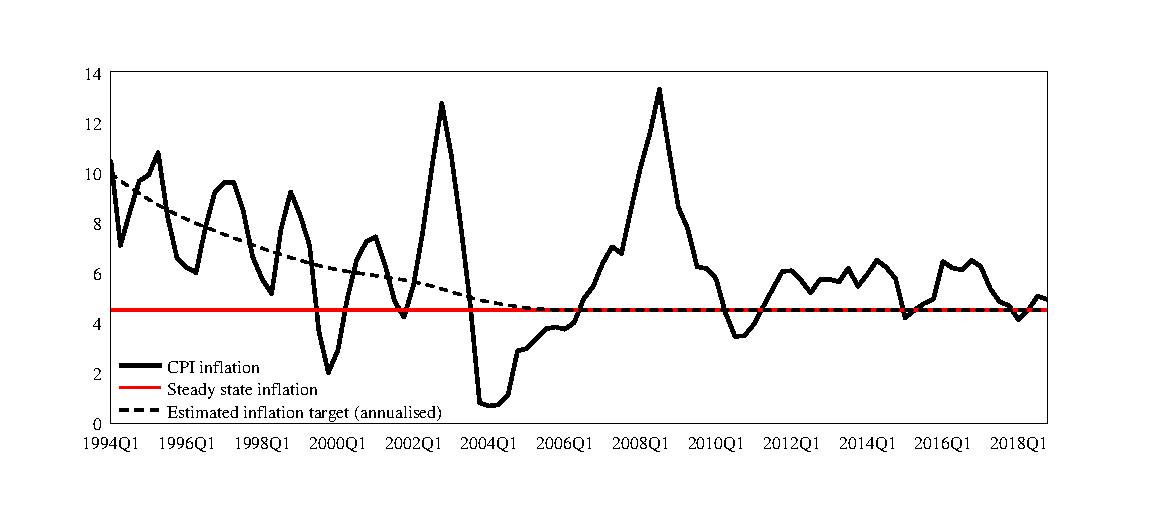
\includegraphics[trim=1.5cm 0.75cm 0 1cm]{cpi_target.eps}\\
			{\footnotesize \textit{Source:} SARB, Author's calculations.}\\
		\end{tabular}
		\label{fig_cpi_target}
	\end{figure} 
	
	\subsection{Calibration}
	
	While the model is estimated using Bayesian techniques, a sizeable share of the parameters is nevertheless calibrated. In particular, those parameters that affect the model's non-stochastic steady state, as well as those parameters that are not suitably identified, are calibrated using external information.\footnote{See the Appendix for details on the computation of the steady state.}\footnote{Identification analysis was carried out in Dynare. The identification procedures  embedded in Dynare toolbox are largely based on \cite{iskrev2010a, iskrev2010b}}.
	
	The model's steady state growth rate, $g_z$, is set equal to 1.0067, which implies a steady state economy-wide growth rate of 2.7\% - roughly	the average growth rate of GDP over the sample. Some of the model's key steady-state ratios are fixed to match their empirical counterparts. These include the expenditure shares of private consumption, private investment, public sector investment and government consumption, which are set equal to 62.2\%, 12.6\%, 5.7\%, and 19.5\% of nominal GDP respectively. The export and import shares are set to 28.2\%, ensuring balanced trade in steady state.
	
	As mentioned above, the steady state rate of inflation in the model, $\bar{\pi}$, is set equal to the mid-point of the SARB's official target band, yielding an annual rate of 4.5\%. Conditional on the model's steady state growth rate and steady state rate of inflation, the discount factor $\beta$ is chosen to be deliver an annualised steady state nominal interest rate of 9.8\% - roughly equal to the average policy interest rate over the sample. Since $R=(\bar{\pi}g_z)/\beta$, this implies that $\beta=0.994$.
	
	The share of private consumption in the aggregate consumption bundle, $\alpha_G$, is set equal to 0.75. This parameter value implies roughly equal marginal utilities of private (Ricardian) consumption and government consumption (\citealp{coenen2013}). On the supply side, the capital share of production is set equal to 0.3, i.e. $\alpha=0.3$. The share of private capital in the CES aggregate, $\alpha_K$, is set equal to 0.9. This ensures roughly equal the marginal products of private and public capital. The depreciation rates for private capital, $\delta$, and public capital, $\delta_G$, are set equal to 0.015 and 0.008 respectively, implying annual deprecation rates of 6\% and 3.5\%. The parameters that govern the adjustment cost of capital utilisation, $\gamma_{u,1}$ and $\gamma_{u,2}$ are calibrated as follows: $\gamma_{u,1}$ is pinned down by the steady state calculation as $\gamma_{u,1}=r_K/\bar{\pi}$, while $\gamma_{u,2}$ is set such that the ratio of the two parameters is equal to 0.1, matching the parameterisation in \cite{steinbach2014}. 
	
	Turning to the fiscal sector, steady-state tax rates are calibrated to match the average effective tax rates in the data, measured as the revenue-to-tax base ratio. Specifically, the steady state values for indirect (or consumption) taxes, $\tau^c$, labour taxes, $\tau^w$, and capital taxes, $\tau^k$, are set equal to 16.7\%, 19.1\%, and 20.3\% respectively. Regarding government debt, the steady-state debt-to-GDP ratio is fixed at 50\% per annum. This is higher than the sample average of approximately 37\%. However, South Africa's debt-to-GDP has increased substantially  over the last decade, from below 25\% in 2008 to close to 60\% in 2018. Given the current low-growth environment and the increasing demands on the fiscus, this trend is likely to continue into the foreseeable future. As such, the steady state debt-to-GDP is calibrated at a relatively conservative 50\% per annum.
	
	The inverse Frisch elasticity of labour supply, $\sigma_L$ is set equal to 5, following \cite{steinbach2014}. As discussed in the Appendix, the shares of domestic production in aggregate consumption and investment, $\nu_C$ and $\nu_I$, are calibrated so as to ensure that the steady state ratios of total imports and exports to GDP match their sample means of roughly 28\%. Following \citealp{steinbach2014}), $\theta_W$ and $\chi_W$ are both set equal to 0.75. The calibration implies that wage contracts are re-optimised once a year, with a relatively high degree of indexation to past inflation. The steady state wage markup, $\phi_W$, follows \cite{adolfson2007} and \cite{steinbach2014} and is calibrated at 1.05, while $\phi_H$ is calibrated to 1.1. The substitution elasticities for consumption, investment and foreign goods and are calibrated to 1.5, 1.5 and 1.25 respectively. Steady state foreign inflation is calibrated to match the sample mean of roughly 2\% per annum.
	
	\begin{table}[t]
		\footnotesize
		\centering
		\captionsetup{skip=6pt}
		\caption{Calibrated parameters}
		\makebox[\linewidth]{
			\begin{tabular}{p{0.5cm} p{4.75cm} p{0.8cm} p{0.5cm} p{6.75cm} p{1cm}} 
				\toprule
				$\beta$ & Discount factor & 0.994 & $g_z$ & Permanent technology growth & 1.0067\\
				$\bar{\pi}$ & Steady state inflation & 1.011 & $\alpha_G$ & Share of private consumption in CES aggregate & 0.75\\
				$\alpha$ & Capital share in production & 0.3 & $\alpha_K$ & Share of private capital in CES aggregate & 0.9 \\
				$\delta$ & Depreciation rate: private capital & 0.015 & $\delta_G$ & Depreciation rate: public capital & 0.008 \\
				$B_Y$ & Government debt-to-GDP ratio & 0.5 & $\sigma_L$ & Labour supply elasticity & 5\\
				$\nu_C$ & Consumption domestic share & 0.64 & $\nu_I$ & Investment domestic share & 0.52 \\ 
				$\theta_W$ & Calvo: wage setting & 0.75 & $\chi_W$ & Indexation: wage setting & 0.75\\
				$\phi_W$ & Wage setting markup & 1.05 & $\phi_H$ & Domestic price markup & 1.1\\
				$\mu_C$ & Subst. elasticity: consumption & 1.5 & $\mu_I$ & Subst. elasticity: investment & 1.5\\
				$\mu^*$ & Subst. elasticity: foreign & 1.25 & $\pi^*$ & Foreign inflation & 1.005 \\ 
				$s_C$ & Private consumption share & 0.622 & $s_I$ & Private investment share & 0.126 \\
				$s_{I_G}$ & Public investment share & 0.057 & $s_G$ & Government consumption share & 0.195\\
				$s_X$ & Export share & 0.282 & $s_{IM}$ & Import share & 0.282\\
				\toprule
			\end{tabular}
		}	
		\label{tab_cal}
	\end{table}
	
	\subsection{Prior distributions}
	
	The prior means for the set of estimated parameters are summarised in Table \ref{tab_prior_est} and Table \ref{tab_prior_est_cont} in the Appendix and largely follows \cite{christoffel2008}, \cite{leeper2010}, \cite{coenen2013}, and \cite{steinbach2014}. 
	
	As the share parameters, $\omega$ and $\bar{\omega}$, are bounded between zero and one, they are assumed to follow a beta distribution. Similarly, the degree of habit persistence is also assumed to follow a beta distribution around 0.65. The prior for the investment adjustment cost parameter, $\phi_i$, follows a normal distribution with a mean of 8. 
	
	Given that the elasticities $\nu_G$ and $\nu_K$ in the CES aggregates for consumption and the capital stock are restricted to be positive, the prior is assumed to follow a gamma distribution with mean 1 (corresponding to the Cobb-Douglass case) and	standard deviation 0.2.
	
	Turning to price setting, the Calvo ($\theta$'s) and indexation parameters ($\chi$'s) are bounded to lie between zero and one and are assumed to follow beta distributions. Importantly, the size of the prior means on the Calvo parameters reflect the stylized fact that inflation is relatively sticky.
	
	Following \cite{smets2003}, among others, the priors for the Taylor rule parameters are fairly standard. However, following \cite{steinbach2014}, a larger weight is placed on both output parameters in order to allow for flexible inflation targeting.
	
	Regarding the feedback coefficients in the fiscal rules, $\theta_{.,Y}$ and  $\theta_{.,B}$, gamma distributions with means of around 0.5 and standard deviations of 0.3 are adopted. For the smoothing coefficients embedded in the fiscal rules, $\rho_{.}$, beta distributions are adopted. 
	
	Finally, the persistence of structural shocks are all assumed to follow a beta distribution	around a mean of 0.85 with standard deviation of 0.1, while the standard deviations of the shocks themselves are assumed to follow inverse-gamma distributions around a mean of 0.1 with standard deviation of 2.
	
	\subsection{Estimation results}
	
	Estimation results are summarised in Table \ref{tab_prior_est}, while Figure \ref{fig_post_dens} presents the prior and posterior distributions. 
	
	The posterior mean of the share of non-Ricardian households is $\omega=0.233$ which is similar to estimates in the literature for developed economies. This relatively low estimate might seem at odds with the stylized facts associated with the South African income distribution. South Africa is a highly unequal society with a large share of the population having little to no access to financial services and/or saving and investment mechanisms. This would point to a larger share of non-Ricardian households in the model set-up. However, individuals in higher income groups also spend more, with the larger share of total consumption expenditure focused in the middle- and top income groups. Given that the model seeks to match the \textit{dynamics} in total consumer spending, combined with the fact that higher-income groups likely dominate aggregate spending dynamics, it would follow that the estimated share of non-Ricardian consumers would be on the low side.
	
	As in \cite{coenen2013}, the model also allows transfer shocks to play a distributional role, the strength of which depends on the share parameter $\bar{\omega}$. However, given an estimate of 0.46, the overall impact is relatively small.
	
	The posterior mean estimate of the elasticity of substitution between private and government consumption goods is $\nu_G = 1.013$, suggesting that the two goods enter the household's utility function as weak substitutes. In contrast, at 0.921, the estimated elasticity of substitution between private and public capital, $\nu_k$, gives rise to modest complementarities in composite capital.    
	
	Turning to other parameters of interest, the investment adjustment cost parameter is substantially higher than the prior mean, while there is a high degree of habit persistence in aggregate Ricardian consumption ($\kappa=0.891$). The estimated Calvo parameters are rather high. These estimates suggest that the Phillips curves within the model are rather flat or, in other words, that the sensitivity of inflation with respect to movements in marginal costs is low. \footnote{That being said, as mentioned in \cite{christoffel2008}, the high estimates for the Calvo parameters do not necessarily imply a high degree of nominal rigidity. The reason is that	the Calvo-style Phillips curve, in general, does not permit the separate identification of nominal and real rigidities which jointly influence the price-setting behaviour of firms. The inclusion of alternative sources of real	rigidities could allow for the re-interpretation of the Calvo parameter estimates without affecting the slope coefficient of the Phillips curve (\citealp{christoffel2008}).} The inflation indexation parameter for domestic prices is estimated around 0.5, i.e. equal weight is place on past inflation relative to the current inflation target. For export and import prices, this weight is smaller than 0.5.
	
	The posterior estimates for the Taylor rule imply a large weight on interest rate stabilisation. In addition, the while the response to changes in inflation is smaller than under the prior, the response to changing output levels is more pronounced. In all, the estimates suggest that while inflation targeting remains the main objective, output fluctuations (and the level of the output gap) also feature in monetary policy decisions.
	
	Turning to the parameters of the fiscal rules, expenditure items are found to react less strongly to movements in output than taxes, with estimates of $\theta_{G,Y}=0.167$, $\theta_{I_G,Y}=0.216$ and $\theta_{TR,Y}=0.204$.\footnote{Note the signs attached to the different coefficients in the fiscal rules above. Both automatic stabilisers and the reaction to debt enter the fiscal rules with negative signs.} In contrast, there is relatively strong evidence of automatic stabiliser in the tax rules, with estimates of $\theta_{W,Y}=0.305$, $\theta_{K,Y}=0.507$ and $\theta_{C,Y}=0.356$. Apart from public sector investment and transfers, debt feedback coefficients are broadly similar across the different expenditure and tax rules, with the mean posterior estimates coming in at around 0.15. In contrast, at $\theta_{I_G,B}=0.554$, the debt feedback coefficient in the public sector investment rule is quite large, suggesting strong use of public sector investment to stabilise public debt. This could reflect the apparent willingness of South African authorities to cut back on infrastructure budgets in the face of worsening fiscal outcomes. 
	
	The estimates for the persistence of shocks indicate that the various technology shocks and risk premium shocks are most persistent, while the fiscal shocks are least persistent. Consistent with the high weight placed on interest rate smoothing, monetary policy shocks display a low degree of volatility. Apart from public sector investment and transfer shocks, export markup shocks are the most volatile, possibly reflecting the large weight of commodities in South Africa's export basket.
	
	\subsection{Identification and sensitivity}
	
	The identification analysis is based on \cite{ratto2008} and \cite{ratto2011}. Weak identification implies that changes in a particular parameter are compensated for by linear combinations of one or more other parameters (\cite{iskrev2010b}), or that changes in a particular parameter have a negligible effect on the model moments (\cite{andrle2010}).
	
	The identification analysis from Figures \ref{fig_ident_pattern}, \ref{fig_ident}, and \ref{fig_sens} in the Appendix shows that all model parameters are identified in the model at the posterior mean. Figure \ref{fig_ident} plots the identification strength at the	posterior mean. Parameters are ranked in increasing order of identification strength. From the top panel in Figure \ref{fig_ident}, we see that all parameters are identified, i.e. no value is exactly zero. 
	
	The bottom panel suggests that all parameters have a non-negligible effect on the first- and second-order moments. Additionally, a desirable characteristic is that the relatively weaker identified parameters have a lesser effect on the model moments (\citealp{hollander2018}).
	
	Finally, the posterior density estimates (Figure \ref{fig_check_plot} in the Appendix) and the convergence diagnostic statistics (Figures \ref{fig_mdiag} and Figure \ref{fig_conv_plot} in the Appendix) show that there is no clear indication of a problem with the optimizer.\footnote{Figure \ref{fig_check_plot} shows the log-posterior likelihood functions and log-likelihood kernels. If the estimated mode is the local mode, it should be at the maximum of the posterior likelihood. Figure \ref{fig_mdiag} and Figure \ref{fig_conv_plot} presents the multivariate and univariate convergence diagnostic statistics (\citealp{brooks1998}). The convergence of the estimates eliminates bimodal or poorly identified parameter distributions.}
	
	\subsection{Model fit and historical decomposition}
	
	Table \ref{tab_moments} compares several theoretical moments implied by the model to those of the observed data series in order to determine how well the model fits the data.  
	
	\begin{table}[h]
		\small
		\centering
		\captionsetup{skip=6pt}
		\caption{Model and data moments}
		\begin{tabular}{p{0.1\linewidth} P{0.12\linewidth} P{0.12\linewidth} P{0.12\linewidth} P{0.12\linewidth} P{0.12\linewidth} P{0.12\linewidth}} 
			\toprule
			& \multicolumn{2}{c}{$\sigma(x_t)$} & \multicolumn{2}{c}{$\rho(x_t,x_{t-1})$} & \multicolumn{2}{c}{$\rho(x_t,y_t)$}  \\
			\cline{2-7}
			& Model & Data & Model & Data & Model & Data  \\
			\hline
			$\Delta\ln(\tilde{Y}_t)$ & 1.875 & 0.600 & 0.194 & 0.534 & 1.000 & 1.000\\
			$\Delta\ln(\tilde{C}_t)$ & 0.971 & 0.706 & 0.523 & 0.748 & 0.184 & 0.630 \\
			$\Delta\ln(\tilde{G}_t)$ & 0.196 & 0.903 & 0.587 & 0.449 & -0.127 & 0.245 \\
			$\Delta\ln(\tilde{I}_t)$ & 3.593 & 2.483 & 0.713 & 0.279 & -0.025 & 0.562 \\
			$\Delta\ln(\tilde{I}_{G,t})$ & 4.433 & 4.311 & 0.431 & 0.364 & 0.005 & 0.135 \\
			$\Delta\ln(\tilde{X}_t)$ & 7.065 & 5.063 & 0.225 & -0.115 & 0.877 & 0.357 \\
			$\Delta\ln(\tilde{M}_t)$ & 2.810 & 3.749 & 0.519 & 0.063 & -0.019 & 0.397 \\
			$\Delta\ln(\tilde{S}_t)$ & 5.115 & 5.538 & -0.005 & 0.226 & 0.306 & 0.039 \\
			$\Delta\ln(\tilde{E}_t)$ & 1.613 & 0.687 & 0.312 & 0.284 &  0.882 & 0.377 \\
			$\Delta\ln(\tilde{W}_t)$ & 1.802 & 1.633 & 0.186 & -0.234 & 0.128 & 0.095 \\
			$\Delta\ln(\tilde{TR}_t)$ & 7.893 & 8.138 & -0.106 & -0.398 & -0.084 & -0.028 \\
			$\Delta\tilde{\tau}^w_t$ & 1.184 & 1.082 & -0.049 & -0.449 & 0.434 & -0.073 \\
			$\Delta\tilde{\tau}^k_t$ & 2.398 & 2.315 & -0.081 & -0.391 & 0.355 & 0.023 \\
			$\Delta\tilde{\tau}^c_t$ & 1.339 & 1.242 & -0.082 & -0.473 & 0.433 & 0.002 \\
			$\tilde{R}_t$ & 1.339 & 0.979 & 0.964 & 0.951 & -0.009 & -0.015 \\
			$\tilde{\pi}_{C,t}$ & 1.298 & 0.794 & 0.747 & 0.622 & -0.122 & -0.016 \\
			$\tilde{\pi}_{H,t}$ & 1.595 & 1.267 & 0.660 & 0.561 & -0.142 & 0.264 \\
			$\tilde{\pi}_{I,t}$ & 1.384 & 1.185 & 0.664 & 0.519 & -0.098 & 0.146 \\
			\toprule
			\multicolumn{7}{p{\linewidth}}{\footnotesize \textit{Note:} Time series $x_t$ are the respective variables in the first column, while $y_t$ denotes the growth rate of output, $\Delta\ln(\tilde{Y}_t)$.}\\
			\multicolumn{7}{p{\linewidth}}{\footnotesize \textit{Source:} Author's calculations.}\\
		\end{tabular}
		\label{tab_moments}
	\end{table}
		
	A comparison of the standard deviations (Columns (2) and (3) in Table \ref{tab_moments}) shows that the model generally predicts a larger degree of volatility than observed in the data, mirroring the results in \cite{steinbach2014}. Nevertheless, the relative magnitudes correspond. An important feature of the model, particularly in an open economy setting, is that volatile variables such as imports, exports and the exchange rate are accurately captured. The same rings true for the main variables of interest in this study, namely the fiscal variables. The model does an admirable job in capturing the volatility in the fiscal variables, including the relatively volatile tax rates.  
	
	Columns (4) and (5) compare the model-implied persistence with the actual persistence observed in the data. Apart from one or two exceptions, the model generally succeeds in matching the persistence observed in the data.
	
	The final two columns of Table \ref{tab_moments} contains the cross-correlation of the selected variables with output growth. There is a large degree of similarity - both in terms of sign and magnitude - between the model generated correlations and those observed in the data. However, the model fails to replicate the (slight) pro-cyclical nature of government spending, private investment and imports observed in the data. That being said, in general the model succeeds in matching the observed data. 
	
	Figure \ref{fig_hist_decom} decomposes the model's estimate of year-on-year GDP growth (relative to the mean) into contributions from each of the estimated structural shocks.\footnote{The demand shock group includes shocks to the domestic risk premium, government consumption and government investment. The technology shock group comprises the permanent technology shock, the transitory technology shock and the investment-specific technology shock, while the markup shock group consists of the wage markup, the domestic price markup and the export price markup shocks. The policy shock group comprises the monetary policy shock as well as shocks to the various fiscal variables. Finally, the foreign shock group includes the external risk premium shock, the import price markup shock, and shocks to the foreign variables, including foreign output.} 
	
	\begin{figure}[t]	
		\captionof{figure}{Historical shock decomposition of GDP growth}
		\makebox[\linewidth]{
			\begin{tabular}{P{20cm}}
				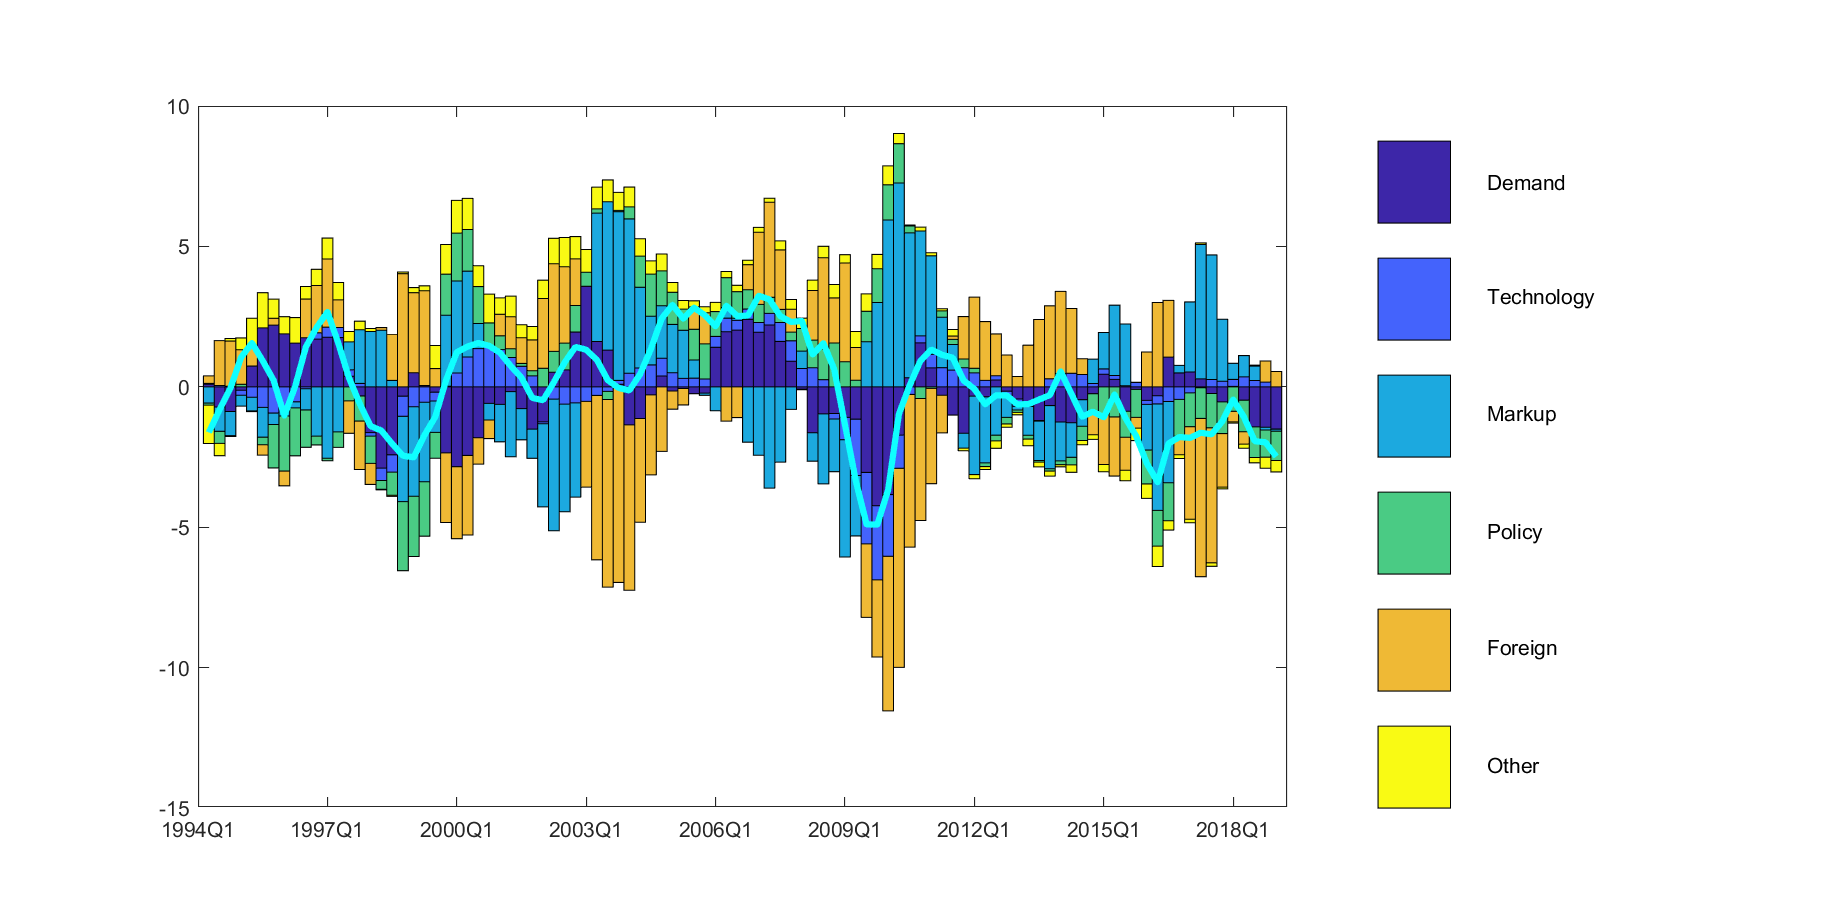
\includegraphics[width=20cm, trim =0 0.5cm 1cm 1.2cm 0, clip]{SAFiscal_shock_decomposition_d4y_obs_group_group1.eps} \\
				{\footnotesize \textit{Source:} Author's calculations.}
			\end{tabular}
		} \label{fig_hist_decom}
	\end{figure}
	
	Developments around the exchange rate, as captured in both the markup and foreign groupings, dominated GDP growth over the period 2000 to 2003, while demand contributed negatively over the same period. This likely reflected increased risk aversion around the turn of the century related to the emerging market crisis of the late 1990s. Between 2006 and 2008, innovations
	to demand and technology contributed positively to growth, while being offset by adverse supply shocks (as captured in the markup group). The negative impact of global developments becomes apparent during the GFC, both through a decline in foreign demand and a shock to export markups. The latter likely reflects the substantial fall in international commodity prices experienced at the time. Additionally, while domestic demand shocks contributed positively to growth in the lead-up to the crisis, the contribution turned negative during the crisis and has remained subdued since. The recovery in the global economy, combined with substantial monetary easing internationally, supported growth between 2012 and 2015. However, the stronger rand exchange rate and drop in commodity prices weighed on export markups. This situation has reversed since 2017, with higher commodity prices and a weaker rand exchange rate countering the slowdown in global growth to some extent. However, the former does not appear to fully offset the negative contributions from domestic demand and less accommodative domestic policy, both monetary and fiscal, over this period.
	
%	\begin{minipage}{\linewidth}

%	\end{minipage}
	
	\subsection{Model dynamics}
	
	Figures \ref{fig_mp} to \ref{fig_ystar} plot impulse responses of key model variables in response to structural shocks common to standard New Keynesian DSGE models. Four distinct shocks are investigated: a shock to the domestic policy interest rate, a transitory technology shock, a shock to the domestic price markup shock, and a shock to foreign demand. The interest rate shock gives information on the monetary policy transmission mechanism, while the other three shocks are examples of supply, cost-push and demand shocks.\footnote{Fiscal policy shocks are discussed in the next section.} 
	
	Figure \ref{fig_mp} presents the response to a one standard deviation interest rate shock. The contractionary policy shock results in the standard response from model variables: a persistent decline across output, consumption, investment and labour, and a dip in inflation. Additionally, in the open economy setting, the appreciation of the domestic currency leads to expenditure-switching from domestic towards foreign goods. The appreciation in the real exchange rate more than offsets the drop in domestic price inflation, resulting in a contraction in exports. Imports also fall, but by less than domestic demand (on impact). The broad-based decline in aggregate demand results in cutback in employment and downward pressure on wages, which translates into lower pricing pressure (through the marginal cost channel). The demand response is aggravated by increased taxes and lower government spending (and transfers) in the face of a rising debt burden. 
	
	Figure \ref{fig_eps} presents the response to a transitory technology shock. The technology shock triggers a decline in marginal cost, which causes domestic prices to fall. Domestic demand adjusts slowly to the increase in supply and, as such, both employment and nominal wages go down. However, the drop in price inflation counters the fall in nominal wages resulting in a slight increase in the real wage. The depreciation of the real exchange rate results in a deterioration in the terms of trade and a concomitant drop in imports and improvement in exports. The rise in import prices results in a smaller decline in CPI inflation relative to domestic prices.
	
	A shock to the domestic price markup, presented in Figure \ref{fig_varphi}, results in a significant increase in domestic price inflation. The concomitant interest rate response lead to a decline in private consumption and investment. The shock to aggregate demand is exacerbated by increased taxes and decreased government spending in the face of rising debt. The appreciation in the real exchange rate results in a drop in exports and improved imports, despite the drop in aggregate demand. The decline in aggregate demand results in a decline in hours worked (employment) and exerts downward pressure on real wages.
	
	A shock to foreign demand (Figure \ref{fig_ystar}), leads to a rise in foreign inflation and the foreign interest rate. The rise in foreign inflation leads to a depreciation in the real exchange rate for the domestic economy. The depreciation in the currency, combined with improved foreign demand conditions, lead to a rise in exports, supporting domestic output growth. The real depreciation also results in lower import demand. Higher inflation abroad reflects in higher import inflation, resulting in higher domestic price inflation and a concomitant tightening of monetary policy.
	
	\begin{minipage}{\linewidth}
		\captionof{figure}{Monetary policy shock}
		\makebox[\linewidth]{
			\begin{tabular}{p{16cm}}
				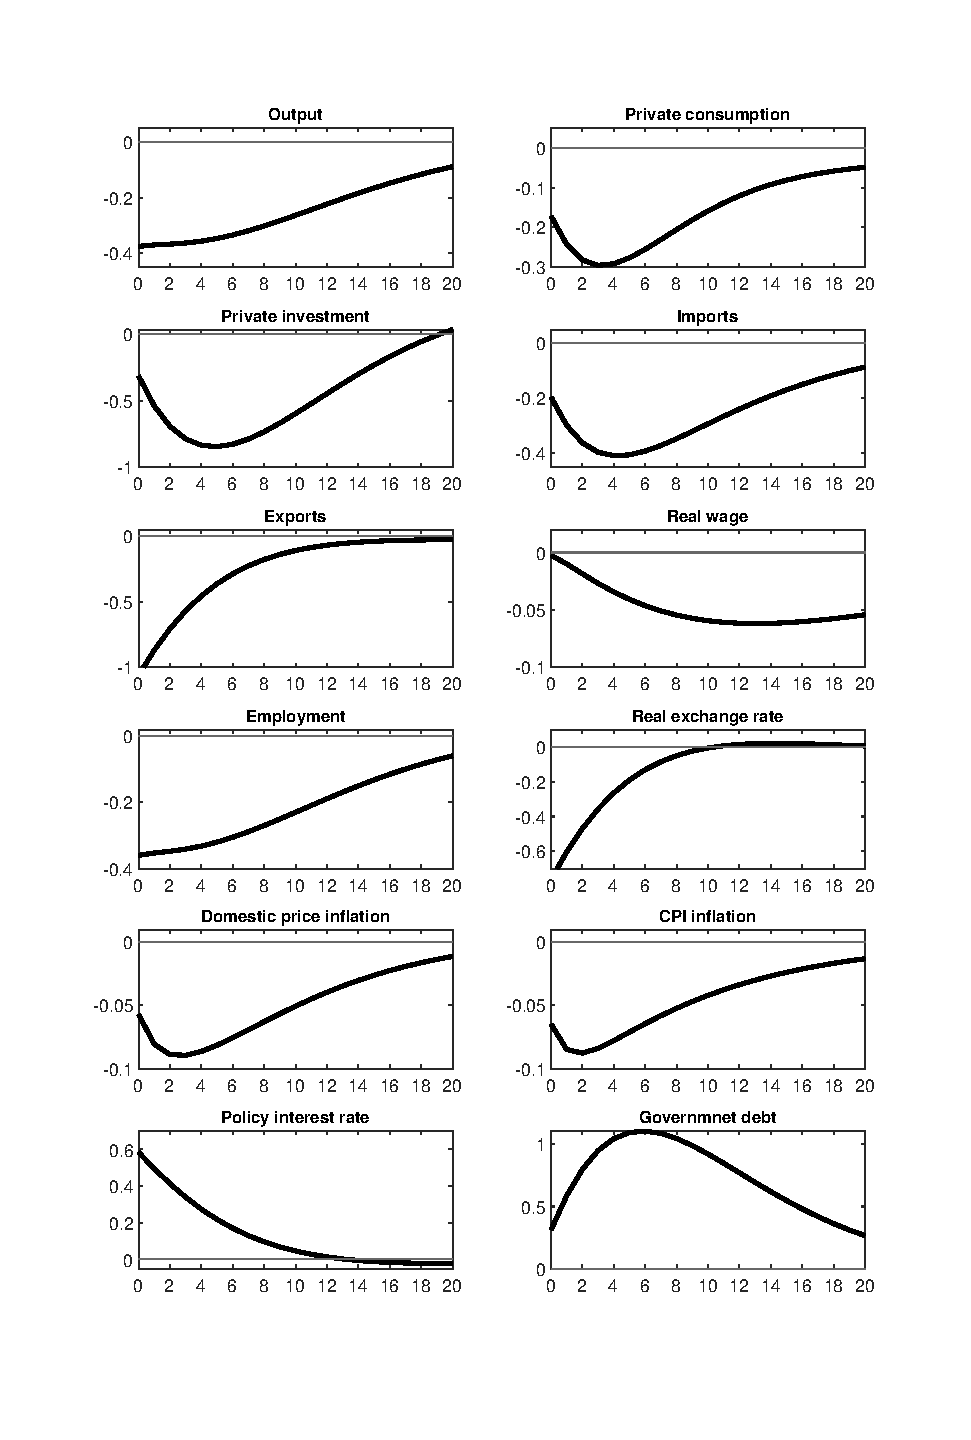
\includegraphics[width=16cm, trim =0 1.75cm 0 0.4cm]{imp_etaR.eps} \\
				{\footnotesize \textit{Note:} All impulse responses are reported as percentage deviations from the non-stochastic steady state, except for inflation rates and the interest rate which are reported as annualised percentage-point deviations.}\\
				{\footnotesize \textit{Source:} Author's calculations.}
			\end{tabular} \label{fig_mp}
		}
	\end{minipage}
	
	\newpage
	\begin{minipage}{\linewidth}
		\captionof{figure}{Transitory technology shock}
		\makebox[\linewidth]{
			\begin{tabular}{p{16cm}}
				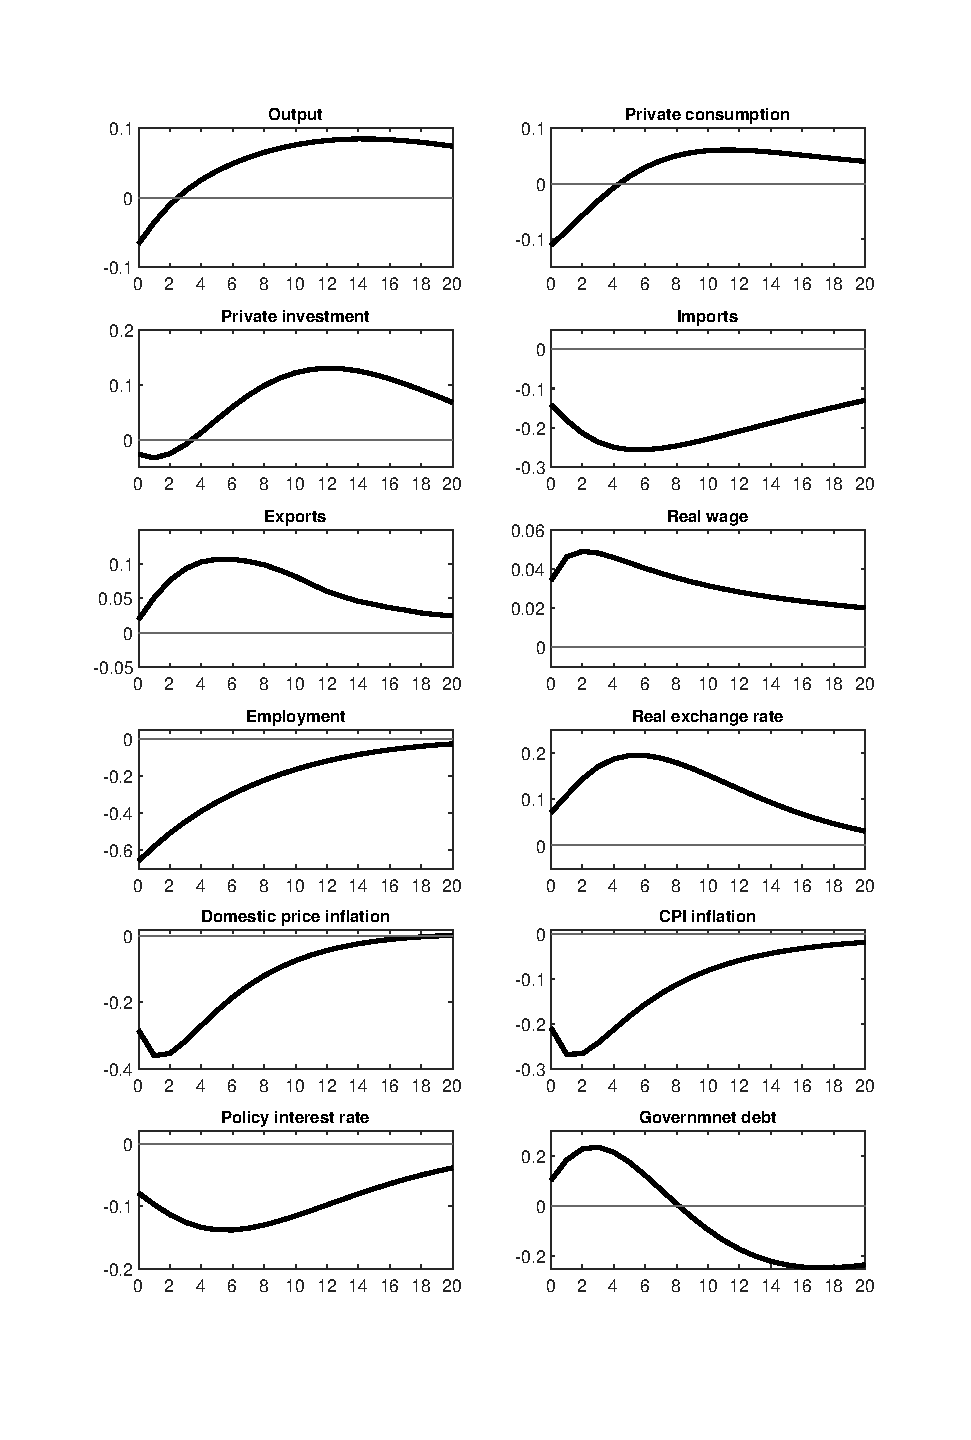
\includegraphics[width=16cm, trim =0 1.75cm 0 0.4cm]{imp_etaeps.eps} \\
				{\footnotesize \textit{Note:} All impulse responses are reported as percentage deviations from the non-stochastic steady state, except for inflation rates and the interest rate which are reported as annualised percentage-point deviations.}\\
				{\footnotesize \textit{Source:} Author's calculations.}
			\end{tabular} \label{fig_eps}
		}
	\end{minipage}
	
	\newpage
	\begin{minipage}{\linewidth}
		\captionof{figure}{Domestic markup shock}
		\makebox[\linewidth]{
			\begin{tabular}{p{16cm}}
				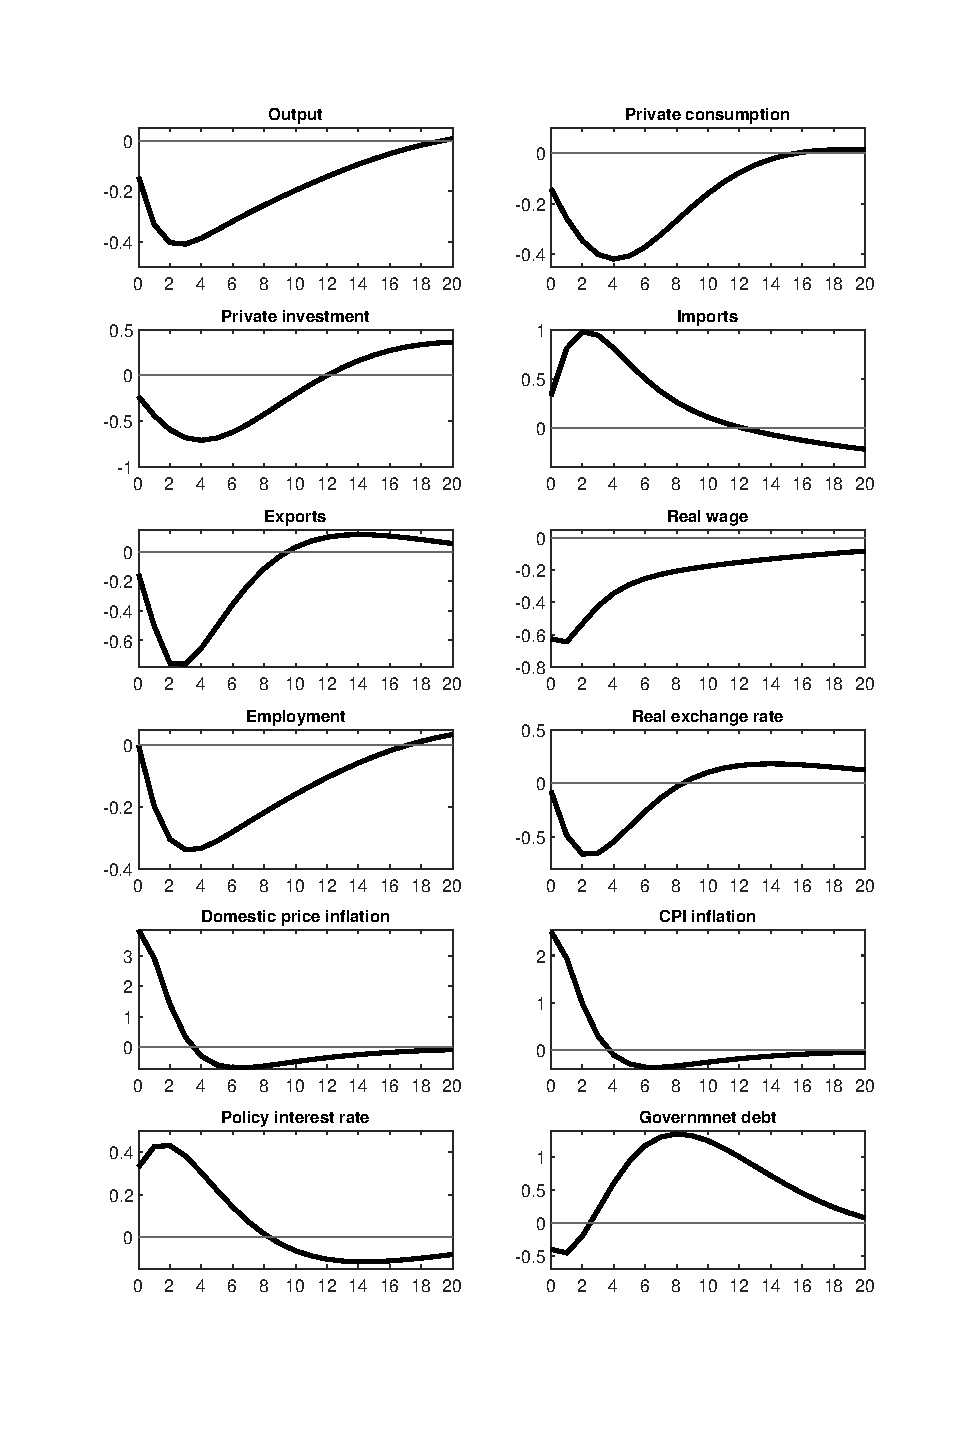
\includegraphics[width=16cm, trim =0 1.75cm 0 0.4cm]{imp_etavarphi.eps} \\
				{\footnotesize \textit{Note:} All impulse responses are reported as percentage deviations from the non-stochastic steady state, except for inflation rates and the interest rate which are reported as annualised percentage-point deviations.}\\
				{\footnotesize \textit{Source:} Author's calculations.}
			\end{tabular} \label{fig_varphi}
		}
	\end{minipage}
	
	\newpage
	\begin{minipage}{\linewidth}
		\captionof{figure}{Foreign output shock}
		\makebox[\linewidth]{
			\begin{tabular}{p{16cm}}
				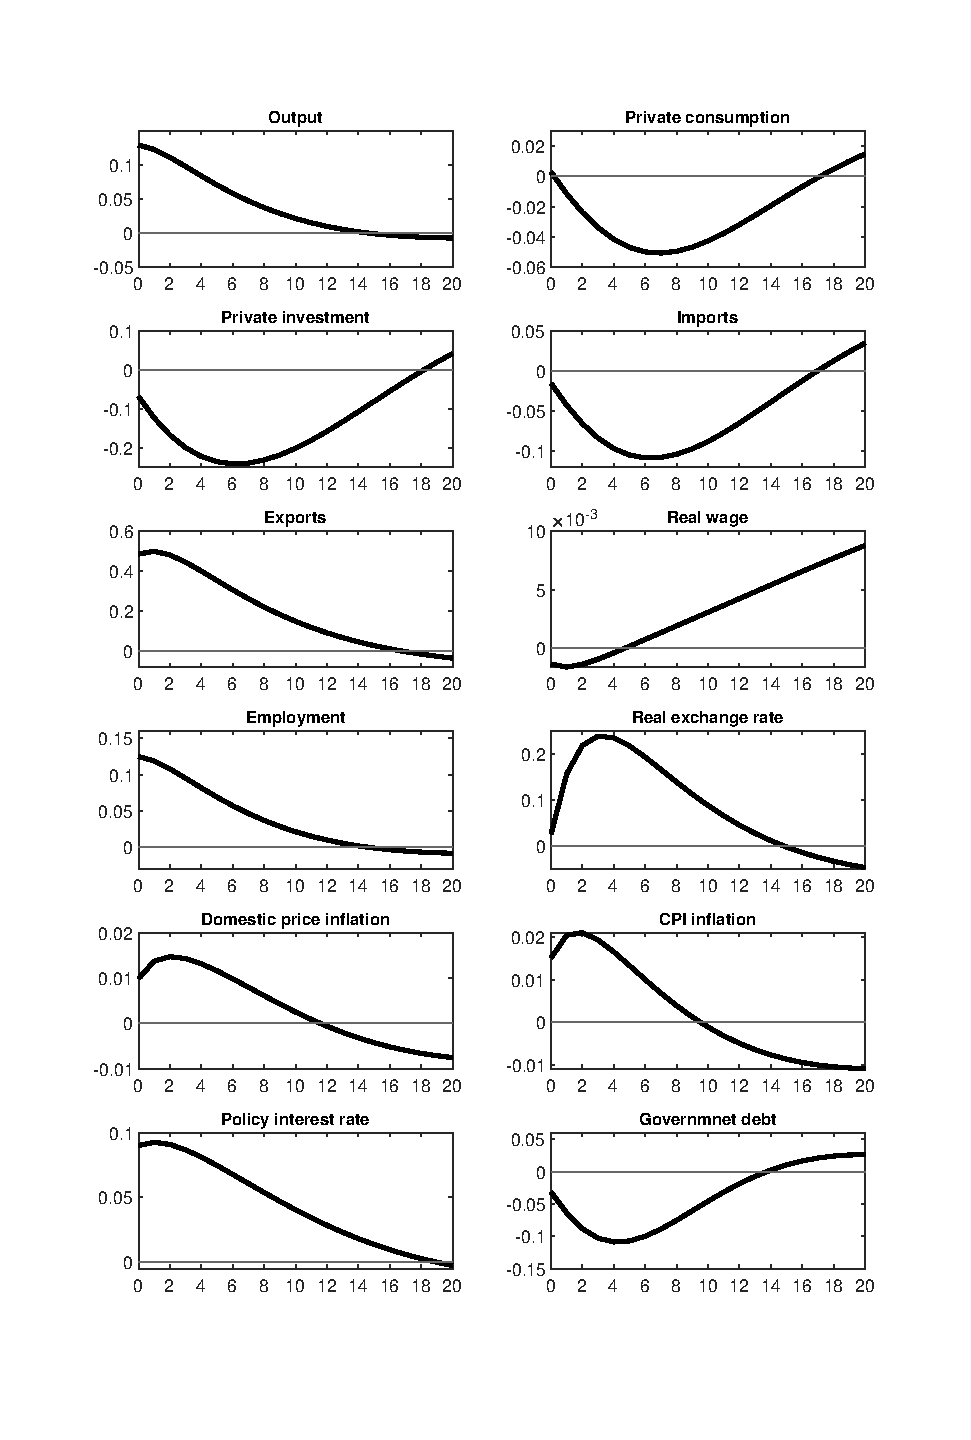
\includegraphics[width=16cm, trim =0 1.75cm 0 0.4cm]{imp_etaYstar.eps} \\
				{\footnotesize \textit{Note:} All impulse responses are reported as percentage deviations from the non-stochastic steady state, except for inflation rates and the interest rate which are reported as annualised percentage-point deviations.}\\
				{\footnotesize \textit{Source:} Author's calculations.}
			\end{tabular} \label{fig_ystar}
		}
	\end{minipage}
	
	\section{The dynamic response to fiscal policy innovations} \label{simulations}
	
	The previous section presented the estimated model and showed that it fit the data reasonably well and responded as expected in response to key structural shocks. This section will explore the response of the model to fiscal shocks. In particular, the response of model variables to different fiscal shocks will be investigated under different debt-financing arrangements. The first subsection investigates the dynamic response to fiscal policy innovations, while the second subsection calculates fiscal multipliers under different scenarios.
	
	\subsection{Impulse responses}
	
	Figures \ref{fig_imp_gcon} to \ref{fig_imp_tauC} plot the impulse responses following a temporary one standard deviation exogenous increase in each fiscal instrument. Each row investigates the responses of a the relevant endogenous variable under different specifications for the fiscal rules. The rules are adjusted by limiting a specific instrument or set of instruments' ability to respond to changing debt levels. That is, the debt feedback coefficients in the fiscal rules are altered. The first column in each figure represents the response of the variable in the model where all fiscal instruments respond to debt. In the second column, only transfers are allowed to respond. The third column gives the results when both government consumption spending and investment respond to debt, while the final column present the case where only tax rates are permitted to respond to debt. In general, as also shown in \cite{leeper2010}, the figures show that the effects of fiscal policy shocks depend crucially on the debt-financing arrangement.
	
	Figure \ref{fig_imp_gcon} shows the responses of output, private consumption, private investment and government debt following a one standard deviation shock to government consumption spending. As is standard in this type of model, an increase in government spending induces a negative wealth effect, leading to an increase in labour supply and hence output. Government spending crowds out private investment, as reflected in the dip in private investment, while the negative wealth effect leads to a drop in consumption. Furthermore, government consumption enters the aggregate consumption good as a substitute to private consumption, thereby exacerbating the negative consumption response. The duration of these effects depends crucially on the debt-financing arrangement embodied in the fiscal rule. When only transfers adjust to stabilise debt, the effects are long-lasting. When only spending variables adjust, output quickly returns to its steady state level as the subsequent decline in government consumption and investment spending in response to rising debt levels weighs on output growth. Under the assumption that only effective tax rates respond to deviations in debt, output returns to its steady state level within five years as tax rates respond to rising debt levels. The negative response of private consumption and investment is long-lasting as the increases in distortionary labour, consumption, and capital taxes weigh on private aggregates.     
	
	The response of model variables to a shock to public sector investment is qualitatively similar (see Figure \ref{fig_imp_ig}). However, as public capital was shown to be a complement to private capital in composite capital good used in private production, the increased public investment expenditure and concomitant increase in public capital results in a slightly more muted (negative) private investment response. Additionally, the private consumption response turns positive after two years due to the reduction in government consumption expenditure in response to rising debt levels. Importantly, the output response following a shock to public sector investment is larger than the response following a shock to government consumption expenditure under all the alternative specifications. This suggests that public sector fixed investment is better suited to stimulating economic activity than current government expenditure.  
	
	\newpage
	\begin{minipage}{\linewidth}
		
		\makebox[\linewidth]{
			\begin{tabular}{P{18cm}}
				\captionof{figure}{Government spending shock}\label{fig_imp_gcon}
				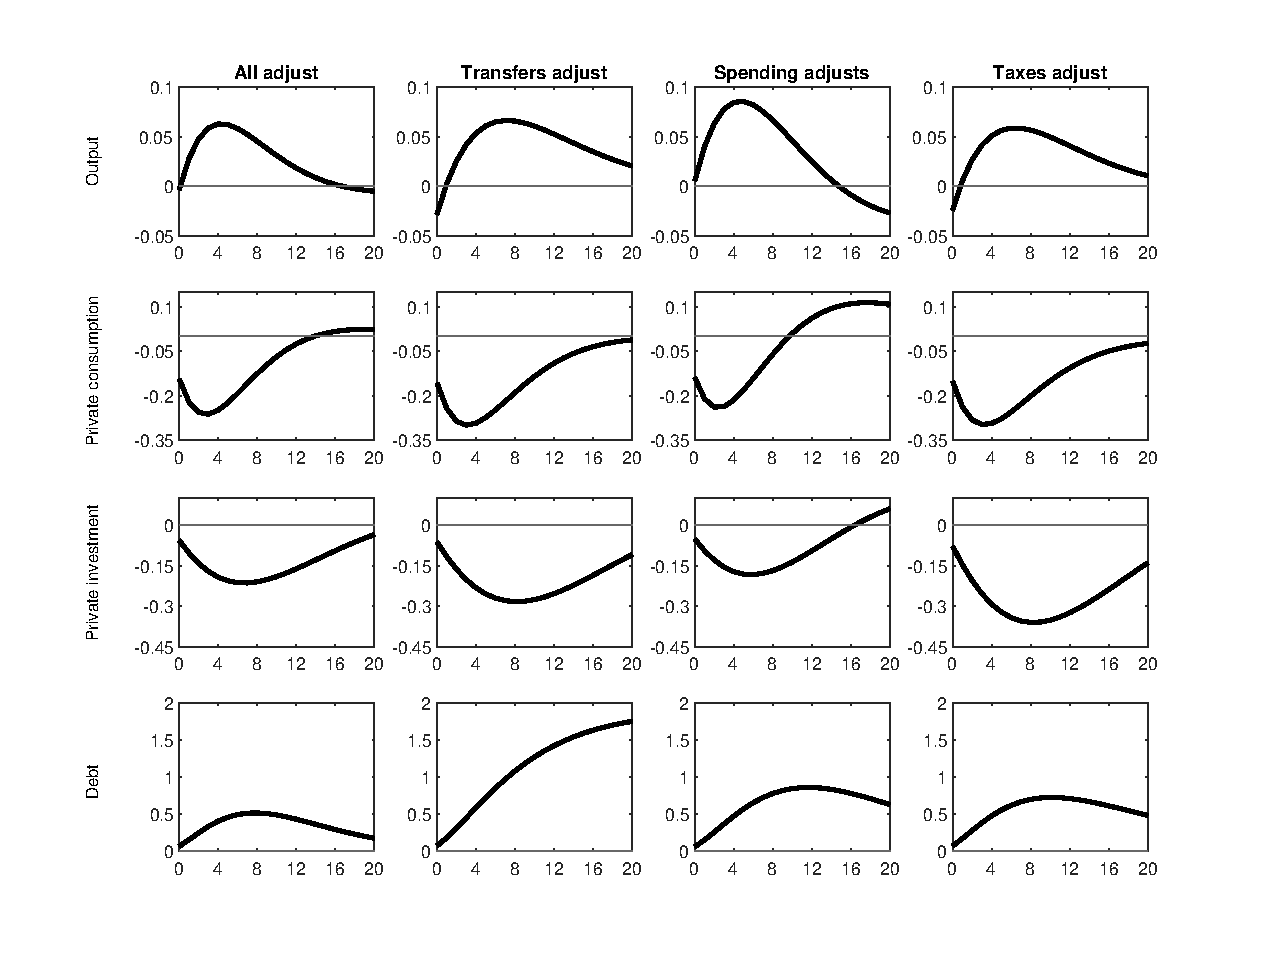
\includegraphics[width=15cm, trim =0 0 0 0.3cm]{imp_etag.eps} \\ 
				\captionof{figure}{Government investment shock}\label{fig_imp_ig}
				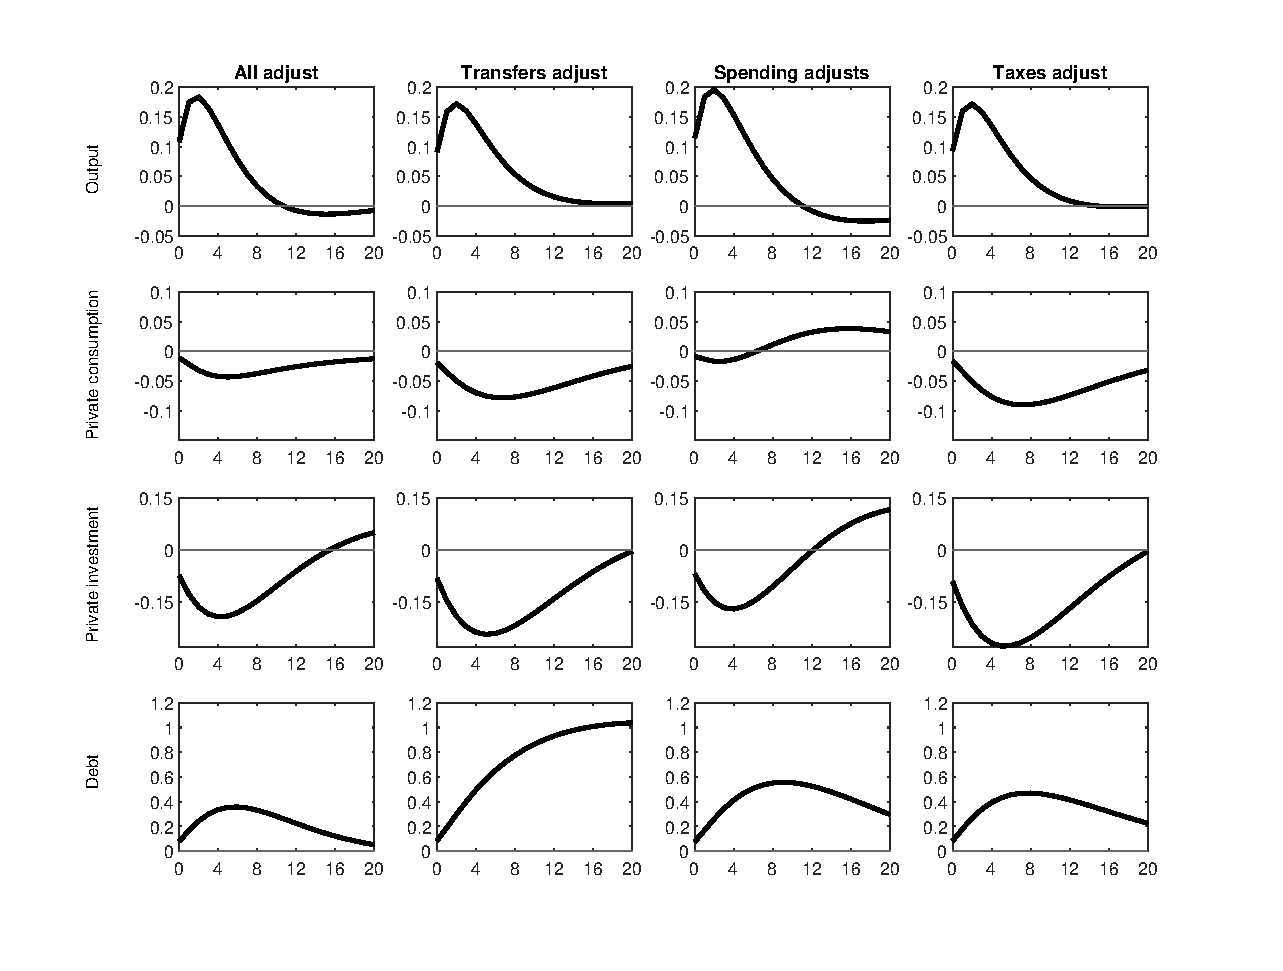
\includegraphics[width=15cm, trim =0 0 0 0.3cm]{imp_etaig.eps}  \\
				{\footnotesize \textit{Source:} Author's calculations.}
			\end{tabular}
			
		}
	\end{minipage}
	
	\newpage
	\begin{minipage}{\linewidth}
		
		\makebox[\linewidth]{
			\begin{tabular}{P{18cm}}
				\captionof{figure}{Labour tax shock}\label{fig_imp_tauN}
				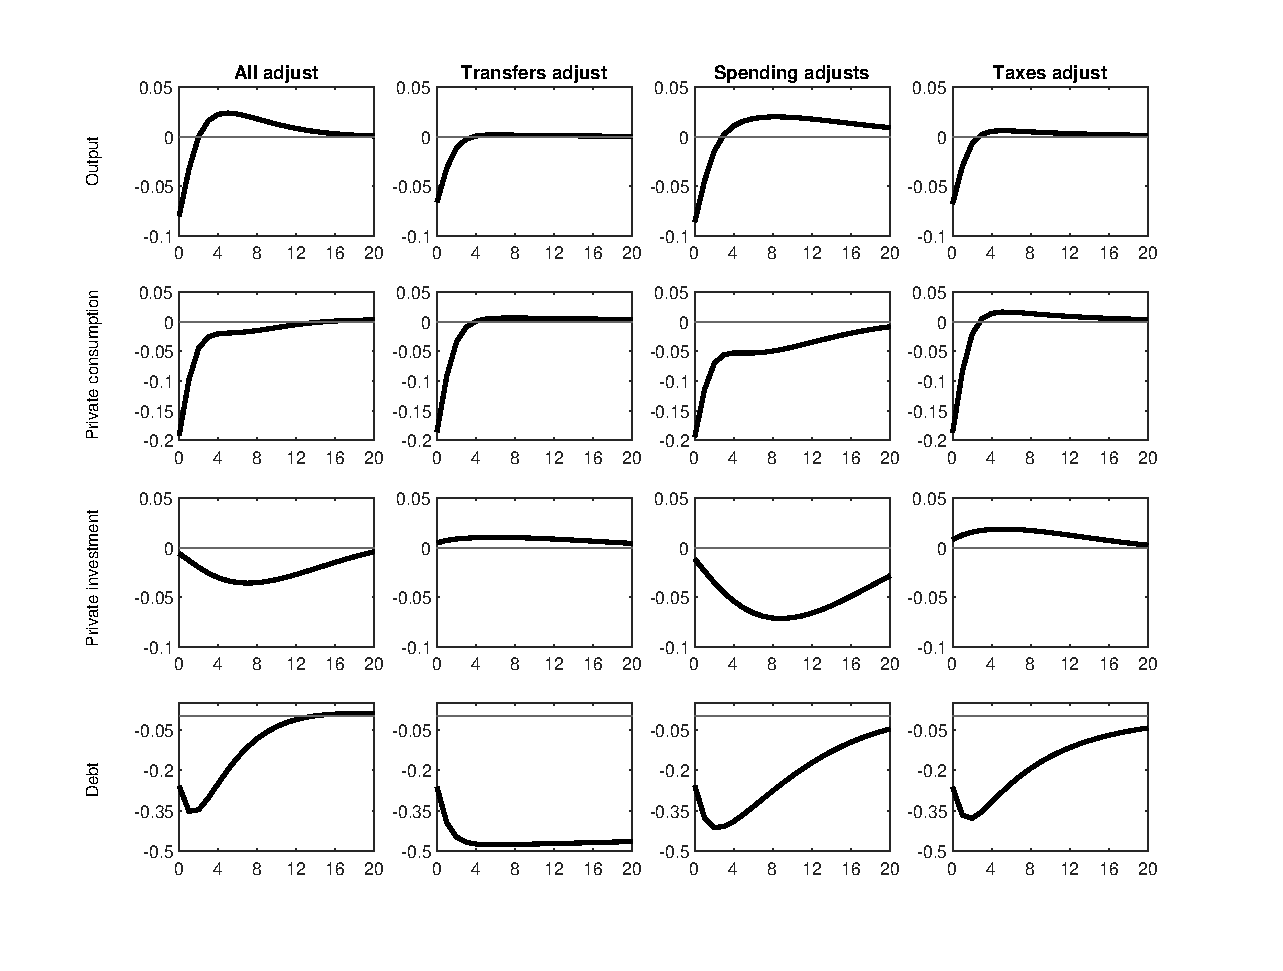
\includegraphics[width=15cm, trim =0 0 0 0.3cm]{imp_etatauN.eps} \\ 
				\captionof{figure}{Capital tax shock}\label{fig_imp_tauK}
				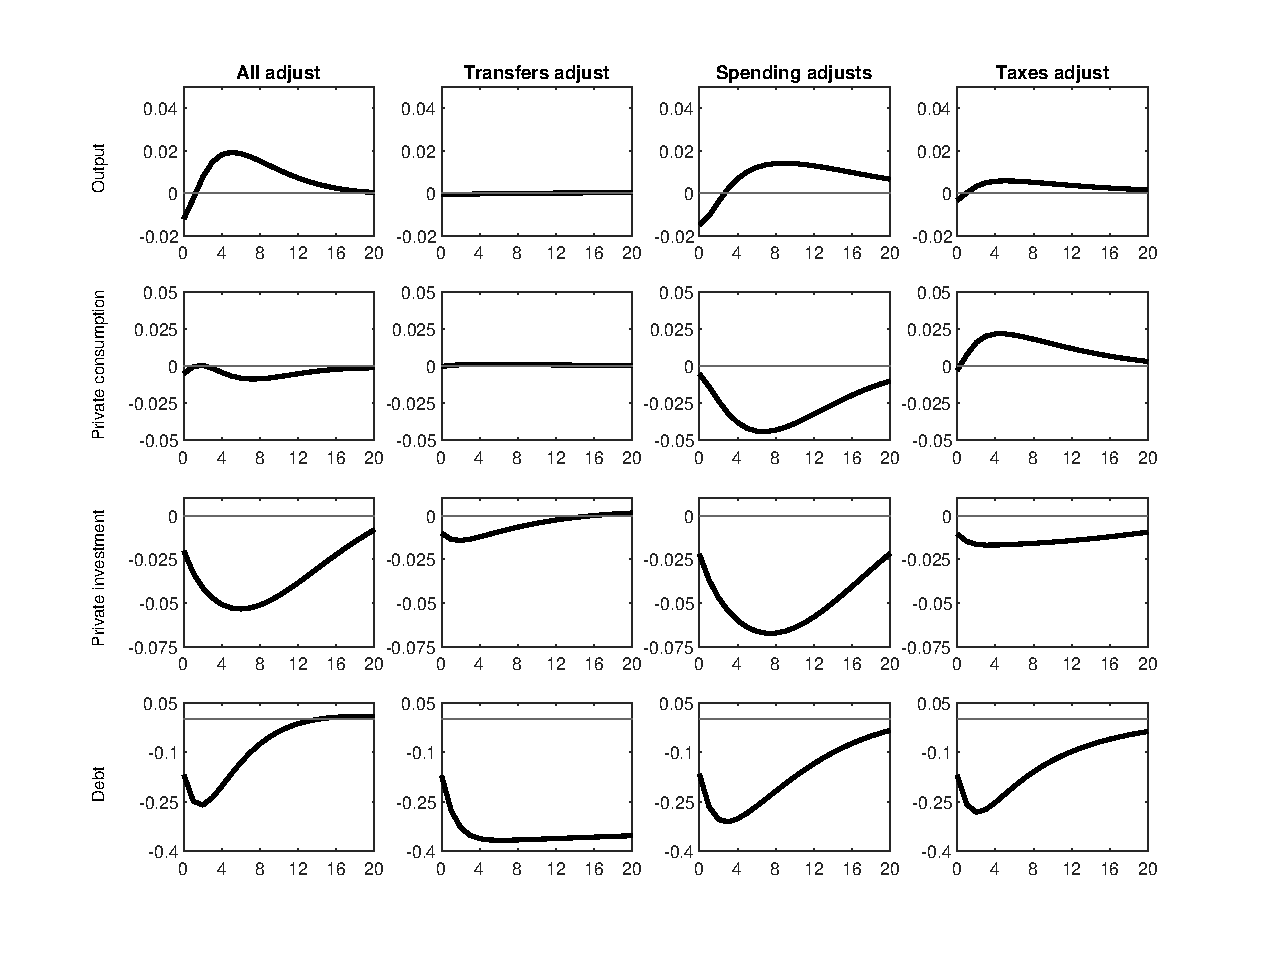
\includegraphics[width=15cm, trim =0 0 0 0.3cm]{imp_etatauK.eps} \\ 
				{\footnotesize \textit{Source:} Author's calculations.}
			\end{tabular}
			
		}
	\end{minipage}
	
	\newpage
	\begin{minipage}{\linewidth}
		\captionof{figure}{Consumption tax shock}
		\makebox[\linewidth]{
			\begin{tabular}{P{18cm}}
				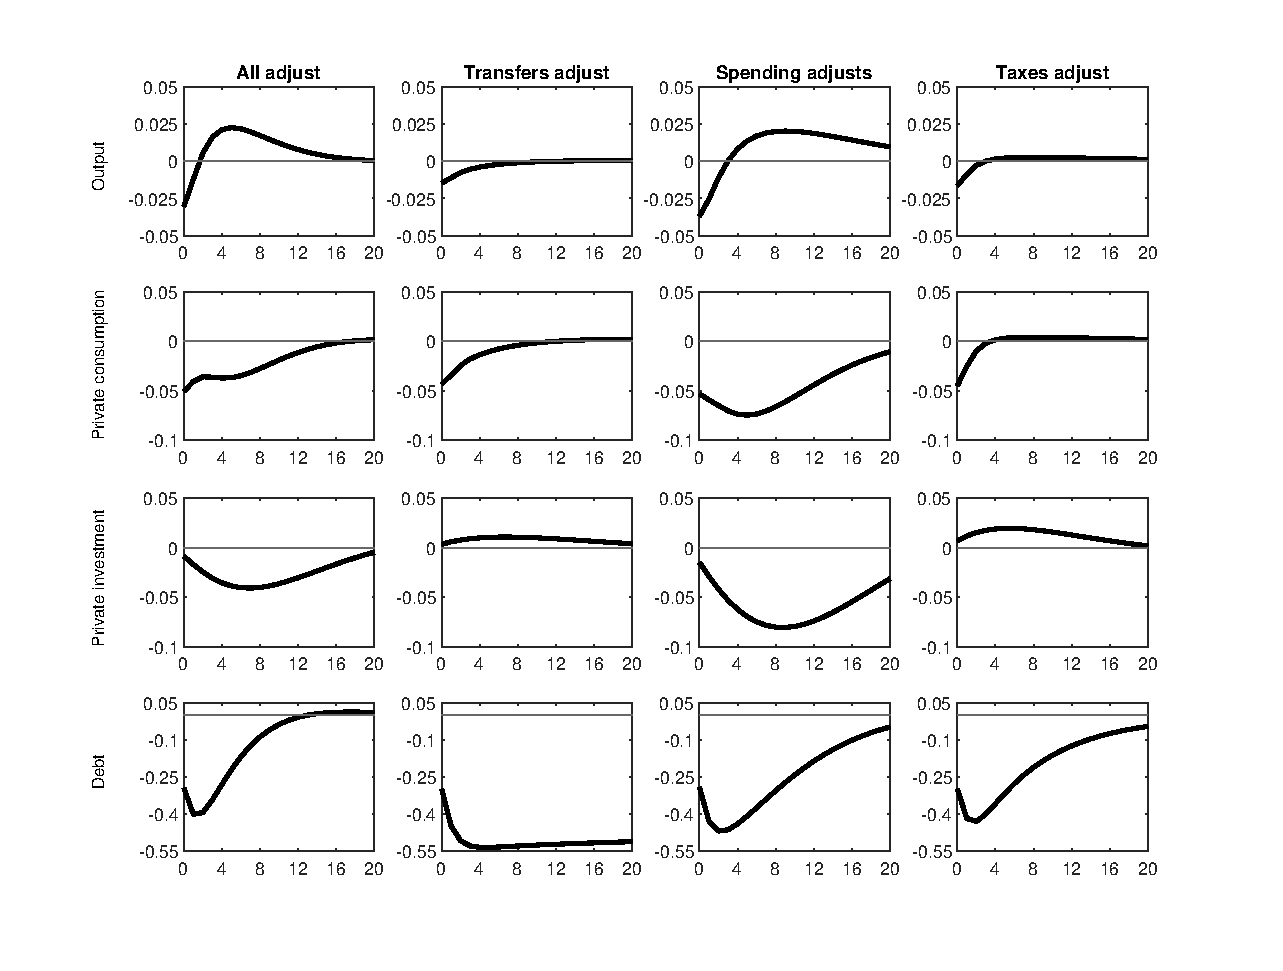
\includegraphics[width=15cm, trim =0 0 0 0.3cm]{imp_etatauC.eps} \\
				{\footnotesize \textit{Source:} Author's calculations.}
			\end{tabular}
			\label{fig_imp_tauC}
		}
	\end{minipage}
	
	Turning to tax shocks, Figure \ref{fig_imp_tauN} reports the effect of a one standard deviation increase in the effective labour tax rate. The responses are broadly intuitive, with higher labour taxes inducing a negative labour supply response, which, in turn, reduces income and consumption. The reduction in labour supply also leads to a reduction in output. Once again, the duration of the effects depends crucially on the debt financing arrangement. It might be expected that investment will also fall since the return to capital drops as households reduce their labour supply. However, under certain financing arrangements the impact might be positive. For example, under the scenario where only taxes adjust to debt, the private investment response is (marginally) positive throughout. This is due to the decline in both consumption and capital tax rates in response to lower government debt levels. 
	
	Figure \ref{fig_imp_tauK} presents the results for a one standard deviation shock to the capital tax rate. Standard theory suggests that an increase in capital taxes induces declines in private investment, labour supply, and output, while consumption rises as agents sacrifice investment for consumption (\citealp{leeper2010}). However, in the current model these responses are not always apparent. As expected, the response of private investment is negative no matter what debt financing arrangement is in place. However, the output and consumption responses depend crucially on which fiscal instruments respond to debt. When all government spending variables adjust, the output response turns positive after about a year as government consumption and investment increase following the decline in government debt. When only taxes adjust, the consumption response is positive as labour and consumption taxes fall, resulting in an \textit{expansion} in output.  
	
	Finally, the response to a shock to consumption taxes is qualitatively similar to those discussed above, although the consumption and investment responses are reversed. An increase in consumption taxes reduce output on impact as consumption declines. The response of private investment depends crucially on the financing arrangement. When only spending variables adjust, the negative wealth effect of the increase in government consumption spending crowds out the effect of increased government investment spending, with the response of both private consumption and investment more pronounced than under other financing arrangements. However, when only tax rates adjust, the drop in capital tax rates result in a positive response for private investment, while the decline in consumption taxes results in a less pronounced negative response from private consumption. 
	
	\subsection{Fiscal multipliers}
	
	The quantitative effects of fiscal policy shocks are summarised using present-value fiscal multipliers. Present value multipliers are calculated as the ratio of the (discounted) \textit{integral} of the output response to the \textit{integral} of the government spending response. That is:
	
	\begin{equation}
	\text{Present-value multiplier at horizon \textit{k}} = \frac{\sum_{j=0}^{k}(1+r)^{-j}y_{t+j}}{\sum_{j=0}^{k}(1+r)^{-j}f_{t+j}}\frac{1}{f/y}
	\end{equation}
	
	where $y_{t+j}$ is the response of GDP component at period $j$, $f_{t+j}$ is the response of the fiscal variable at period $j$, and $r$ is the average (model consistent) nominal policy interest rate over the sample. As before, the responses are scaled by $f/y$ (the ratio of the fiscal variable to real GDP evaluated at the sample mean). The tax response is measured as the response in total tax revenue (that is $f$ is equal to labour, capital and consumption tax \textit{revenue} when investigating the impact of unanticipated tax shocks). Present-value fiscal multipliers under the scenario when all fiscal variables respond to debt are presented in Table \ref{pv_all_tools}. 
	
	\begin{table}[h!]
		\small
		\centering
		\captionsetup{skip=6pt}
		\caption{Present-value multipliers: All instruments respond}
		\begin{tabular}{p{2cm} P{1.25cm} P{1.25cm} P{1.25cm} P{1.25cm} P{1.25cm}} 
			\toprule
			Variable& Q1 & Q4 & Q8 & Q20 & $\infty$ \\
			\hline
			\multicolumn{6}{l}{\textbf{Government consumption multiplier}} \\
			\hline
			$\frac{\Delta Y}{\Delta G}$ & -0.04 & 0.19 & 0.21 & 0.20 & 0.20\\
			$\frac{\Delta C}{\Delta G}$ & -0.82 & -0.72 & -0.64 & -0.55 & -0.55\\
			$\frac{\Delta I}{\Delta G}$ &-0.07 & -0.08 & -0.10 & -0.12 & -0.11\\
			\hline
			\multicolumn{6}{l}{\textbf{Government investment multiplier}} \\
			\hline
			$\frac{\Delta Y}{\Delta I_G}$ &0.56&0.62&0.57&0.51&0.51\\
			$\frac{\Delta C}{\Delta I_G}$ &-0.04&-0.07&-0.09&-0.12&-0.12\\
			$\frac{\Delta I}{\Delta I_G}$ &-0.05&-0.07&-0.09&-0.09&-0.09\\
			\hline
			\multicolumn{6}{l}{\textbf{Labour tax multiplier}} \\
			\hline
			$\frac{\Delta Y}{\Delta T^w}$ &-0.42&-0.28&-0.13&-0.04&-0.04\\
			$\frac{\Delta C}{\Delta T^w}$ &-0.62&-0.75&-0.88&-0.91&-0.91\\
			$\frac{\Delta I}{\Delta T^w}$ &0.00&-0.03&-0.07&-0.10&-0.10\\
			\hline
			\multicolumn{6}{l}{\textbf{Capital tax multiplier}} \\
			\hline
			$\frac{\Delta Y}{\Delta T^k}$ &-0.15&0.10&0.36&0.49&0.49\\
			$\frac{\Delta C}{\Delta T^k}$ &-0.04&-0.04&-0.11&-0.17&-0.18\\
			$\frac{\Delta I}{\Delta T^k}$ &-0.03&-0.13&-0.22&-0.31&-0.31\\
			\hline
			\multicolumn{6}{l}{\textbf{Consumption tax multiplier}} \\
			\hline
			$\frac{\Delta Y}{\Delta T^c}$ &-0.19&-0.04&0.14&0.24&0.24\\
			$\frac{\Delta C}{\Delta T^c}$ &-0.19&-0.41&-0.60&-0.68&-0.68\\
			$\frac{\Delta I}{\Delta T^c}$ &-0.01&-0.05&-0.09&-0.13&-0.13\\
			\toprule
			\multicolumn{6}{l}{\footnotesize \textit{Source:} Author's calculations.}\\
		\end{tabular}
		\label{pv_all_tools}
	\end{table}
	
	Output multipliers are positive for both government spending and investment shocks. Importantly, the positive output multipliers are smaller than one across the board, although the public sector investment multiplier is significantly larger than the spending multiplier. Government spending and investment shocks crowd out private consumption and investment, resulting in relatively small multipliers. Consumption multipliers are negative following both a labour and consumption tax shock, while investment responds negatively to a capital tax shock. The positive output multipliers following a capital tax shock reflects the drop in tax rates and the expansion in public spending and investment in response to falling debt levels.
	
	Present value multipliers under other financing arrangements broadly follow the intuition of the impulse response analysis above (details are presented in Tables \ref{pv_spend_tools} and \ref{pv_tax_tools}). Shocks to government investment consistently produce larger and more persistent positive effects on output (in present value terms). In contrast, labour and consumption taxes are highly distortionary, resulting in relatively persistent declines in output and consumption.
	
	\subsection{Consumption multipliers and non-Ricardian households}
	
	As mentioned earlier, a key driver of positive output multipliers in response to government spending shocks in the empirical literature is the finding that consumption reacts positively to shocks to government consumption spending. However, the evidence does not universally support the idea that higher government spending raises private consumption. In fact, the structural model in the current paper does not point to positive consumption multipliers, despite the addition of rule-of-thumb consumers.
	
	That being said, the estimated share of non-Ricardian households in the current model set-up is quite low. The question is whether a larger share of non-Ricardian household could generate positive consumption multipliers. Table \ref{pv_omega} presents present-value output and consumption multipliers following a shock to government spending for different assumptions regarding the share of non-Ricardian households. \footnote{The table presents results for the baseline model where all fiscal instruments respond to stabilise debt, but the results are qualitatively similar for other financing arrangements.}
	
	\vspace{6pt}
	\begin{table}[h]
		\small
		\centering
		\captionsetup{skip=6pt}
		\caption{Present-value multipliers for different values of $\omega$}
		\begin{tabular}{p{2cm} P{1.25cm} P{1.25cm} P{1.25cm} P{1.25cm} P{1.25cm}} 
			\toprule
			& Q1 & Q4 & Q8 & Q20 & $\infty$ \\
			\hline
			\multicolumn{6}{l}{$\omega=0.233$ (baseline estimate)} \\
			\hline
			$\frac{\Delta Y}{\Delta G}$ & -0.04 & 0.19 & 0.21 & 0.20 & 0.20\\
			$\frac{\Delta C}{\Delta G}$ & -0.82 & -0.72 & -0.64 & -0.55 & -0.55\\
			\hline
			\multicolumn{6}{l}{\textbf{$\omega=0.50$}} \\
			\hline
			$\frac{\Delta Y}{\Delta I_G}$ &0.07&0.29&0.30&0.27&0.27\\
			$\frac{\Delta C}{\Delta I_G}$ &-0.574&-0.51&-0.49&-0.45&-0.45\\
			\hline
			\multicolumn{6}{l}{\textbf{$\omega=0.75$}} \\
			\hline
			$\frac{\Delta Y}{\Delta T^w}$ &0.20&-0.42&0.41&0.35&0.34\\
			$\frac{\Delta C}{\Delta T^w}$ &-0.27&-0.28&-0.30&-0.34&-0.35\\
			\hline
			\multicolumn{6}{l}{\textbf{$\omega=0.90$}} \\
			\hline
			$\frac{\Delta Y}{\Delta T^k}$ &0.29&0.51&0.49&0.40&0.38\\
			$\frac{\Delta C}{\Delta T^k}$ &-0.07&-0.11&-0.18&-0.28&-0.30\\
			\toprule
			\multicolumn{6}{l}{\footnotesize \textit{Source:} Author's calculations.}\\
		\end{tabular}
		\label{pv_omega}
	\end{table}
	
	While the implied multipliers do increase with the share of non-Ricardian households, consumption multipliers never turn positive, while the output multipliers remain well below one. This finding is consistent with evidence for open economies (see, for example, \citealp{ratto2006}; \citealp{forni2009}; \citealp{naitram}; \citealp{sin2016}). Additionally, the introduction of additional frictions in the model set-up in the form of labour and consumption taxes (which respond to debt), serves to dampen the effect of government spending increases.
	
	\subsection{Dynamics of debt financing}
	
	Another question that arises relates to the efficacy of the different fiscal instruments in restoring steady-state level debt following a fiscal policy innovation. Figure \ref{fig_imp_debt} plots the response of government debt to a one standard deviation innovation in government consumption spending.\footnote{The results are shown for a shock to government spending. While the relative magnitudes and duration differ according to the initial shocked fiscal variable, the general conclusions hold for other shocks.} Each line represents the impulse if only that specific fiscal instrument adjusts to changes in government debt.
	
	It is clear that a spending shock results in a persistent deviation in debt from its steady state level, regardless of the financing method. Even in the case where all instruments respond collectively, it takes several years for debt to return to its steady state level. In terms of the individual fiscal instruments, the most effective consolidation tools appear to be government consumption spending, and labour and consumption taxes. In contrast, government investment spending and capital taxes appear to be ineffective at brining debt back to its steady state level, even over a longer time period. The long-lasting impact of fiscal policy innovations on debt is well-documented in the literature (see \citealp{leeper2010} for a particularly well-constructed contribution). 
	
	\begin{minipage}{\linewidth}
		
		\makebox[\linewidth]{
			\begin{tabular}{P{15cm}}
				\captionof{figure}{Debt financing dynamics}\label{fig_imp_debt}
				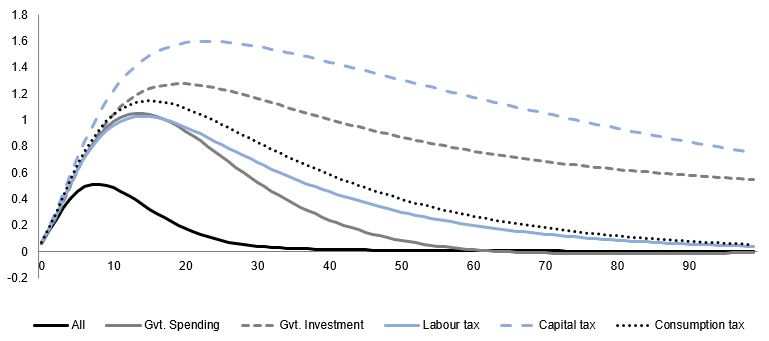
\includegraphics[width=15cm, trim =0 0 0 0]{Debt.jpg} \\ 
				{\footnotesize \textit{Source:} Author's calculations.}
			\end{tabular}
		}
	\end{minipage}
	
	\subsection{The role of automatic stabilisers}
	
	Assumptions regarding the role of automatic stabilisers also play an important role in debt dynamics. In the baseline results discussed above, the coefficients measuring the contemporaneous response of fiscal variables to output were set at their estimated values (as shown in Table \ref{tab_prior_est} in the Appendix ). 

	Figure \ref{fig_stab_debt} presents government debt dynamics following a shock to government consumption spending and assuming all fiscal instruments adjust to stabilise debt. The figure shows results for four different assumptions regarding the automatic response of fiscal instruments to output fluctuations: no automatic response, estimated response, twice the estimated response, and three times the estimated response.
	
	Stronger automatic responses reduce short-run fluctuations, as reflected in the more muted short-term response of debt to the spending shock. However, stronger automatic responses could impose other long-run costs. Higher government spending raises output, which, under the estimated fiscal rules, indices an increase in capital and labour taxes and a decline in transfers. This, in turn, lowers output. This dynamic is more pronounced under stronger automatic stabilisers. The decline in output over the longer term reduces tax revenues, resulting a slightly more persistent deviation from steady state debt (see Figure \ref{fig_stab_debt}).   
	
	\begin{minipage}{\linewidth}
		\makebox[\linewidth]{
			\begin{tabular}{P{15cm}}
				\captionof{figure}{Role of automatic stabilisers in debt dynamics}\label{fig_stab_debt}
				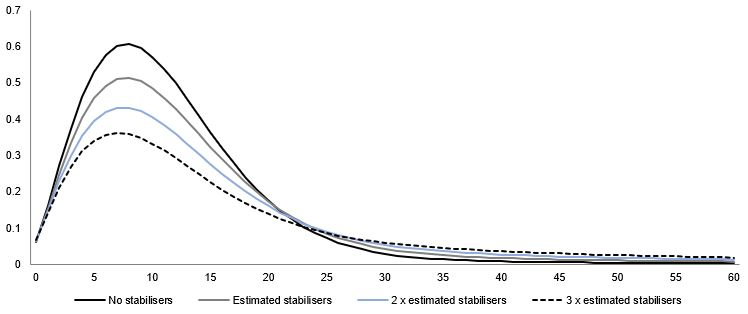
\includegraphics[width=15cm, trim =0 0 0 0]{Auto_stab.jpg} \\
				{\footnotesize \textit{Source:} Author's calculations.}
			\end{tabular}
		}
	\end{minipage}
	
	
	
	\section{Conclusion} \label{con_dsge}
	
	In this paper, an open-economy fiscal DSGE model for the South African economy was constructed. The model includes a detailed fiscal block, as well as several other characteristics that make estimation feasible. 
	
	The estimated model fits the data reasonably well and was used to simulate the effect of innovations to the different fiscal instruments on macroeconomic aggregates, including GDP, private consumption and investment. The results highlight the fact that the fiscal policy process is highly complex and that the impact of fiscal policy decisions on macroeconomic aggregates depends crucially on assumptions about which fiscal instruments adjust to stabilise debt. 
	
	Policy simulations indicate that government spending and investment multipliers are generally positive, albeit smaller than one. Multipliers are also generally smaller than the estimates presented reduced-form modelling approaches, consistent with the idea that spending multipliers are smaller in open-economy settings. Secondly, the estimates indicate that taxes are highly distortionary, with large negative multipliers for private consumption and investment. In contrast, the impact of tax shocks on output is highly ambiguous, with assumptions regarding which instruments adjust to debt and the size of automatic stabilisers playing an important role. Finally, a look at debt dynamics indicates that government consumption spending and, to a slightly lesser extent, labour and consumption taxes are the most effective instruments for stabilising debt after a fiscal shock. This highlights an important finding: cuts in government consumption expenditure, combined with some measure of tax increases, present the most effective options when it comes to the need for fiscal consolidation. 
	
	That being said, conclusions about the effects of fiscal policy depend crucially on the nature of the underlying fiscal rules. As such, it is important for the researcher, and policy maker, to understand the different dynamics under different assumptions regarding the functional form of said rules.  
	
	This paper provides some insight into how fiscal policy decisions affect the economy. While the underlying dynamics are complex, the rules are relatively simple and the model economy could be expanded to include even more realistic assumptions. These could include distinguishing between productive and unproductive government spending, detailed modelling of monetary	policy behaviour, regime-switching fiscal policy, expanding the model to account for differing trends in fiscal variables, and introducing fiscal foresight in the open-economy setting.\footnote{\cite{jooste2017} incorporate an ad hoc measure of fiscal foresight in a calibrated, closed-economy DSGE model for South Africa.} Additionally, the analysis could be extended in order to consider optimal fiscal rules, as well as the differentiated impact of permanent versus temporary innovations to fiscal instruments. 
	
\newpage
\thispagestyle{plain}
\nocite{}
\bibliographystyle{chicago}
\bibliography{bib}

\newpage
\appendix 

\setcounter{table}{0} \renewcommand{\thetable}{A.\arabic{table}}
\setcounter{section}{0}
\setcounter{subsection}{0}
\renewcommand{\thesection}{A.\arabic{section}}  

\setcounter{equation}{0}
\renewcommand\theequation{A.\arabic{equation}}	 

\section*{Appendix} \label{app}

\section{The log-linearised model} 
	
	\subsection{Transformation of variables}
		
	Following \cite{christoffel2008} and \cite{adolfson2007}, among others, the model's structural relationships are cast into stationary form. This is done for two reasons: First, because it is assumed that underlying productivity growth follows a unit-root process, all real variables, with the exception hours worked, have a common real stochastic trend. Second, since the main aim of monetary policy is to stabilise inflation as opposed to the price level, nominal variables share a common nominal stochastic trend. In order to cast the model into stationary form, all real variables that share a common stochastic trend are scaled with the level of productivity, $z_t$, while all nominal variables are scaled by the price level of the consumption good, $P_{C,t}$. For notational simplicity, stationary variables are denoted by lower-case letters. For example, $y_t=Y_t/z_t$ denotes the stationary level of aggregate output, while $p_{I,t}=P_{I,t}/P_{C,t}$ represents the relative price of the investment good.
	
	% as opposed to the upper-case letters employed the discussion in Chapter \ref{ch4}
	
	That being said, there are a few exceptions. First, the nominal wage rate is assumed to grow in line with productivity and, as such, it needs to be scaled by both the price level, $P_{C,t}$, and the productivity level, $z_t$, in order to become stationary, i.e. $w_t = W_t/(z_t P_{C,t})$. Second, given that the model's endogenous state variables, such as the capital stock, are predetermined in a given period $t$, they they need to be scaled by the \textit{lagged} value of productivity, that is, $k_t = K_t/z_{t-1}$. Third, following \cite{christoffel2008}, the marginal utility of consumption needs to be scaled \textit{up} with the level of productivity to become stationary ($\lambda_t = z_t\Lambda_t$). Finally, foreign variables are scaled with the real foreign productivity trend, denoted by $z_t^*$. Furthermore, it is assumed that $z_t$ and $z_t^*$ share the same stochastic trend. 
	
	The following sections present the log-linearised equations characterising the model.
	
	\subsection{Households}
	
	Since all households make identical decisions in equilibrium, the household-specific indices $i$ and $j$ can be dropped. However, superscripts are used to distinguish between Ricardian (R) and non-Ricardian (NR) household variables. 
	
	\subsubsection{Ricardian households}

	\vspace{8pt}
	\textit{The households' choice of allocations}
	\vspace{8pt}
	
	{\color{red} The log-linear version of the expression for aggregate Ricardian consumption eq.~\ref{cons} does not appear in Appendix but it is in the code. Also, it does not look like Ricardian households benefit from government consumption, since they do not optimize and their budget constraint (analogous to Ricardian HHs) does not include $G_t$ (see \ref{nr_budget}?}
	
	Applying the transformation detailed above to the households'
	first-order conditions (\ref{foc_c}) to (\ref{foc_bstar}) yields the following equivalent stationary conditions:
	
	\begin{equation}
	\lambda_t=\alpha_G^{\frac{1}{\nu_G}}\varepsilon_t^c\frac{\left(\tilde{c}_t^R-\kappa g_{z,t}^{-1}\tilde{c}_{t-1}^R\right)^{-1}}{1+\tau_t^c}\left(\frac{\tilde{c}_t^R}{c_t^R}\right)^{\frac{1}{\nu_G}}
	\end{equation}
	
	\begin{multline}
	p_{I,t} = Q_t\varepsilon_t^i\left(1-\Gamma_I\left(g_{z,t}i_t^R/i_{t-1}^R\right)-\Gamma_I^'\left(g_{z,t}i_t^R/i_{t-1}^R\right)g_{z,t}\frac{i_t^R}{i_{t-1}^R}\right)\\+\beta E_t\left[\frac{\lambda_{t+1}}{\lambda_t}Q_{t+1}\varepsilon_{t+1}^i\Gamma_I^'\left(g_{z,t+1}i_{t+1}^R/i_{t}^R\right)g_{z,t+1}\left(\frac{i_{t+1}^R}{i_{t}^R}\right)^2\right]
	\end{multline}
	
	\begin{multline}
	Q_t=\beta E_t\Bigg[\frac{\lambda_{t+1}}{\lambda_t}g_{z,t+1}^{-1}\Big((1-\delta)Q_{t+1} \\ +(1-\tau_{t+1}^k)r_{K,t+1}u_{t+1}+\left(\tau_{t+1}^k\delta-\left(1-\tau_t^k\right)\Gamma_u(u_{t+1})\right)p_{I,t+1}\Big)\Bigg]
	\end{multline}
	
	\begin{equation}
	r_{K,t}=\Gamma_u^'(u_t)p_{I,t+1}
	\end{equation}
	
	\begin{equation} 
	\beta\varepsilon_t^{RP}R_tE_t\left[\frac{\lambda_{t+1}}{\lambda_t}g_{z,t+1}^{-1}\pi_{C,t+1}^{-1}\right]=1
	\end{equation}
	
	\begin{equation} 
	\beta\left(1-\Gamma_{B^*}\left(s_{B^*,t+1};\varepsilon_t^{RP^*}\right)\right)R^*_tE_t\left[\frac{\lambda_{t+1}}{\lambda_t}g_{z,t+1}^{-1}\pi_{C,t+1}^{-1}\frac{s_{t+1}}{s_t}\frac{\pi_{Y,t+1}}{\pi^*_{Y,t+1}}\right]=1
	\end{equation}
	
	where $p_{I,t}=P_{I,t}/P_{C,t}$ is the relative price of the investment good, $r_{K,t}=R_{K,t}/P_{C,t}$ is the real rental rate of capital, {\color{red}{$s_t=S_{t}P^*_{Y,t}/P_{Y,t}$ is the real exchange rate defined in terms of domestic and foreign output deflators. [lower case $s_t$ is confusing---especially in the code---change to $RER_t$ or $\tilde{S}_t$; also, $S_t$ is sometimes used for terms-of-trade]}} $\pi_{Y,t}=P_{Y,t}/P_{Y,t-1}$ and $\pi^*_{Y,t}=P_{Y^*,t}/P_{Y^*,t-1}$ denotes, respectively, domestic and foreign gross inflation rates. 
	
	The stationary capital accumulation equation (\ref{capital}) is given by:
	
	\begin{equation} \label{trans_cap}
	k_{t+1}^R=(1-\delta)g_{z,t}^{-1}k_t^R+\varepsilon_t^i\left(1-\Gamma_I\left(g_{z,t}i_t^R/i_{t-1}^R\right)\right)i_t^R
	\end{equation}
	
	where $k_t^R=K_t^R/z_{t-1}$. 
	
	The transformation of the adjustment cost function (\ref{cap_adj}) yields the following expression, using the fact that the foreign risk premium (\ref{rp_foreign}) and capital utilisation cost functions (\ref{cap_util_cost}) are already in stationary form:
	
	\begin{equation} \label{adj_trans}
	\Gamma_I\left(g_{z,t}i_t^R/i_{t-1}^R\right)=\frac{\gamma_I}{2}\left(g_{z,t}\frac{i_t^R}{i_{t-1}^R}-g_z\right)^2
	\end{equation}
	
	The log-linearised versions of the transformed first order conditions stated above are given by:
	
	\begin{equation}
	\hat{\lambda}_t=-\frac{1}{1-\kappa g_z^{-1}}\hat{\tilde{c}}_t^R+\frac{\kappa g_z^{-1}}{1-\kappa g_z^{-1}}\hat{\tilde{c}}_{t-1}^R-\frac{\kappa g_z^{-1}}{1-\kappa g_z^{-1}}\hat{g}_{z,t}-\frac{1}{1+\tau^c}\hat{\tau}_t^c+\frac{1}{\nu_G}\left(\hat{\tilde{c}}_t^R-\hat{c}_t^R\right)+\hat{\varepsilon}_t^c
	\end{equation}
	
	\begin{equation}
	\hat{p}_{I,t}=\hat{Q}_t+\hat{\varepsilon}^I_t+\gamma_Ig^2_z\left(\beta\left(E_t\left[\hat{i}^R_{t+1}\right]-\hat{i}^R_t\right)-\left(\hat{i}^R_t-\hat{i}^R_{t-1}\right)+\beta E_t\left[\hat{g}_{z,t+1}\right]-\hat{g}_{z,t}\right)
	\end{equation}
	
	\begin{multline}
	\hat{Q}_t=\frac{\beta(1-\delta)}{g_z}E_t\left[\hat{Q}_{t+1}\right]+E_t\left[\hat{\lambda}_{t+1}\right]-\hat{\lambda}_t-E_t\left[\hat{g}_{z,t+1}\right]\\-\frac{\beta(1-\tau^K)r_K}{g_z}E_t\left[\frac{1}{1-\tau^K}\hat{\tau}^K_{t+1}-\hat{r}_{K,t+1}\right]+\frac{\beta\delta p_I}{g_z}E_t\left[\tau^K\hat{p}_{I,t+1}+\hat{\tau}^K_{t+1}\right]
	\end{multline}
	
	\begin{equation}
	\hat{r}_{K,t}=\frac{\gamma_{u,2}}{\gamma_{u,1}}\hat{u}_t+\hat{p}_{I,t}
	\end{equation}
	
	\begin{equation} \label{log_b}
	E_t\left[\hat{\lambda}_{t+1}\right]-\hat{\lambda}_t-E_t\left[\hat{g}_{z,t+1}\right]+\hat{r}_t-E_t\left[\hat{\pi}_{C,t+1}\right]+\hat{\varepsilon}_t^{RP}=0
	\end{equation}
	
	\begin{multline} \label{log_bstar}
	E_t\left[\hat{\lambda}_{t+1}\right]-\hat{\lambda}_t-E_t\left[\hat{g}_{z,t+1}\right]+\hat{r}^*_t-E_t\left[\hat{\pi}_{C,t+1}\right]\\+E_t\left[\hat{s}_{t+1}\right]-\hat{s}_t+E_t\left[\hat{\pi}_{Y,t+1}-\hat{\pi}^*_{Y,t+1}\right]-\gamma_{B^*}\hat{s}_{B^*,t+1}-\hat{\varepsilon}^{RP^*}_t=0
	\end{multline}
	
	After substituting for the transformed adjustment cost function in (\ref{trans_cap}), the log-linearised capital accumulation equation is given by:
	
	\begin{equation}
	\hat{k}_{t+1}=(1-\delta)g^{-1}_z\hat{k}_t-(1-\delta)g^{-1}_z\hat{g}_{z,t}+(1-(1-\delta)g^{-1}_z)\hat{\varepsilon}^i_t+(1-(1-\delta)g^{-1}_z)\hat{i}_t
	\end{equation}
	
	Combining the log-linearised first-order conditions for the domestic and foreign bond holdings, (\ref{log_b}) and (\ref{log_bstar}), yields the following risk-adjusted uncovered interest parity (UIP) condition:
	
	\begin{equation}{\color{red} \label{Eq:UIPloglin}
	\hat{r}_t-\hat{r}^*_t+\hat{\varepsilon}^{RP}_t=E_t\left[\hat{s}_{t+1}\right]-\hat{s}_t+E_t\left[\hat{\pi}_{Y,t+1}-\hat{\pi}^*_{Y_t+1}\right]-\gamma_{B^*}\hat{s}_{B^*,t+1}-\hat{\varepsilon}^{RP^*}_t }
	\end{equation}
	
	\vspace{8pt}
	\textit{Wage setting and aggregate wage dynamics}
	\vspace{8pt}
	
	Aggregate wage dynamics is determined by a wage Phillips curve. Let $\hat{\bar{\pi}}_{C,t}=\text{log}\left(\bar{\pi}_{C,t}/\bar{\pi}_C\right)$ denote the log-deviation of the monetary authority's inflation objective from its long-run value, and recall that $w_t=W_t/\left(z_tP_{C,t}\right)$. Using these definitions and combining the log-linearised first-order condition characterising the optimal wage-setting decision (\ref{foc_wh}) and the log-linearised aggregate wage index (\ref{agg_w}) yields the following log-linear expression for the wage Phillips curve:
	
	\begin{multline} \label{a_wage}
	\hat{w}_t=\frac{\beta}{1+\beta}E_t\left[\hat{w}_{t+1}\right]+\frac{1}{1+\beta}\hat{w}_{t-1}+\frac{\beta}{1+\beta}E_t\left[\hat{\pi}_{C,t+1}\right]\\
	-\frac{1+\beta\chi_W}{1+\beta}\hat{\pi}_{C,t}+\frac{\chi_W}{1+\beta}\hat{\pi}_{C,t-1}-\frac{\beta(1-\chi_W)}{1+\beta}E_t\left[\hat{\bar{\pi}}_{C,t+1}\right]\\
	+\frac{1-\chi_W}{1+\beta}\hat{\bar{\pi}}_{C,t}-\frac{(1-\beta\theta_W)(1-\theta_W)}{(1+\beta)\theta_W\Psi(\phi^W,\sigma_L)}\left(\hat{w}^{\tau}_t-\widehat{mrs}_t-\hat{\phi}^W_t\right)
	\end{multline}
	
	where the terms 
	
	\begin{equation*}
	\hat{w}^{\tau}_t=-\frac{\hat{\tau}^w_t}{1-\tau^w}+\hat{w}_t
	\end{equation*}
	
	\begin{equation*}
	\widehat{mrs}_t=\hat{\varepsilon}^n_t+\sigma_L\hat{N}_t-\hat{\lambda}_t
	\end{equation*}
	
	denote the tax and productivity-adjusted real wage, and the household's marginal rate of substitution between consumption and leisure, respectively. 
	
	Finally, 
	
	\begin{equation*}
	\Psi(\phi^W,\sigma_L)=1+\frac{\phi^W}{\phi^W-1}\sigma_L
	\end{equation*} 
	
	\subsubsection{Non-Ricardian households}
	
	With respect to household budget constraints and non-Ricardian household consumption, it is enough to log-linearise the non-Ricardian budget constraint (\ref{nr_budget}):
	
%	\begin{equation}
%	\left(1+\tau^c\right)\hat{c}^{NR}\left(\frac{\tau^c}{1+\tau^c}\hat{\tau}_t^c+\hat{c}_t^{NR}\right)-\left(1-\tau^w\right)wN\left(\frac{\tau^w}{1-\tau^w}\hat{\tau}_t^w+\hat{w}_t+\hat{N}_t\right)-\hat{tr}_t^{NR} = 0
%	\end{equation}
	
	\begin{equation}
	\left(1+\tau^c\right)\hat{c}^{NR}\left(\frac{1}{1+\tau^c}\hat{\tau}_t^c+\hat{c}_t^{NR}\right)-\left(1-\tau^w\right)wN\left(\frac{1}{1-\tau^w}\hat{\tau}_t^w+\hat{w}_t+\hat{N}_t\right)-\hat{tr}_t^{NR} = 0
	\end{equation}
	
	\subsection{Firms}
	\subsubsection{Domestic intermediate-good firms}
	
	This section derives the log-linear equations characterising the behaviour of intermediate-good producers. For ease of exposition, combined with the fact that all firms make identical decisions in equilibrium, the subscript $f$ is dropped.
	
	\vspace{8pt}
	\textit{Technology, inputs and marginal cost}
	\vspace{8pt}
	
	The stationary production function (\ref{prod_func}) is given by:
	
	\begin{equation}
	y_t=\varepsilon_t\left(g_{z,t}^{-1}\tilde{k}_t\right)^{\alpha}N_t^{1-\alpha}-\psi
	\end{equation}
	
	Similarly, the transformation of (\ref{comb_foc}) yields the following stationary version of the firm's first order condition:
	
	\begin{equation}
	\frac{r_{K,t}}{w_t}=\frac{\alpha}{1-\alpha}\frac{g_{z,t}N_t}{k_t^s}\left[1+\left(\frac{1-\alpha_K}{\alpha_K}\right)^{\frac{1}{\nu_K}}\left(\frac{k_{G,t}}{k_t^s}\right)^{\frac{\nu_K-1}{\nu_K}}\right]^{-1}
	\end{equation}
	
	while the transformation of the marginal cost schedule (\ref{mc}) gives:
	
	\begin{equation}
	mc_t=\frac{1}{\varepsilon_t\alpha^{\alpha}(1-\alpha)^{1-\alpha}}\left(r_{K,t}\right)^{\alpha}\left(w_t\right)^{1-\alpha}\left(\frac{k_t^s}{\tilde{k}_t}\right)^{\alpha}\left[1+\left(\frac{1-\alpha_K}{\alpha_K}\right)^{\frac{1}{\nu_K}}\left(\frac{k_{G,t}}{k_t^s}\right)^{\frac{\nu_K-1}{\nu_K}}\right]^{\alpha}
	\end{equation}
	
	Log-linearised these equations results in the following expressions for the production technology, the first-order condition and the marginal cost schedule:
	
	\begin{equation}
	\hat{y}_t=\left(1+\psi y^{-1}\right)\left(\hat{\varepsilon}_t+\alpha\left(\hat{\tilde{k}}_t-\hat{g}_{z,t}\right)+\left(1-\alpha\right)N_t\right)
	\end{equation}
	
	\begin{equation}
	\hat{r}_{K,t}=\hat{g}_{z,t}+\hat{N}_t+\hat{w}_t-\hat{k}_t^s-\frac{\nu_K-1}{\nu_K}\left[\frac{\left(\frac{1-\alpha_K}{\alpha_K}\right)^{\frac{1}{\nu_K}}\left(\frac{k_G}{k^s}\right)^{\frac{\nu_K-1}{\nu_K}}}{1+\left(\frac{1-\alpha_K}{\alpha_K}\right)^{\frac{1}{\nu_K}}\left(\frac{k_G}{k^s}\right)^{\frac{\nu_K-1}{\nu_K}}}\right]\left(\hat{k}_{G,t}-\hat{k}_t^s\right)
	\end{equation}
	
	\begin{equation}
	\hat{mc}_t=-\hat{\varepsilon}_t+\alpha\hat{r}_{K,t}+(1-\alpha)\hat{w}_t+\alpha\left(\hat{k}_t^s-\hat{\tilde{k}}_t\right)+\alpha\frac{\nu_K-1}{\nu_K}\left[\frac{\left(\frac{1-\alpha_K}{\alpha_K}\right)^{\frac{1}{\nu_K}}\left(\frac{k_G}{k^s}\right)^{\frac{\nu_K-1}{\nu_K}}}{1+\left(\frac{1-\alpha_K}{\alpha_K}\right)^{\frac{1}{\nu_K}}\left(\frac{k_G}{k^s}\right)^{\frac{\nu_K-1}{\nu_K}}}\right]\left(\hat{k}_{G,t}-\hat{k}_t^s\right)
	\end{equation}
	
	Public capital accumulation is analogous to that for private capital and is given by
	
	\begin{equation}
	\hat{k}_{G,t+1}=(1-\delta)g^{-1}_z\hat{k}_{G,t}-(1-\delta)g^{-1}_z\hat{g}_{z,t}+(1-(1-\delta)g^{-1}_z)\hat{\varepsilon}^i_t+(1-(1-\delta)g^{-1}_z)\hat{i}_{G,t}
	\end{equation}
	
	Finally, the log-linear version of the expression for aggregate capital used in production is
	
	\begin{equation}
	\hat{\tilde{k}}_t=\alpha_K^{\frac{1}{\nu_K}}\left(\frac{k^s}{\tilde{k}}\right)^{\frac{\nu_K-1}{\nu_K}}\hat{k}_t^s+(1-\alpha_K)^{\frac{1}{\nu_K}}\left(\frac{k_G}{\tilde{k}}\right)^{\frac{\nu_K-1}{\nu_K}}\hat{k}_{G,t}
	\end{equation}
	
	\vspace{8pt}
	\textit{Price setting and price dynamics}
	\vspace{8pt}
	
	The domestic and export Phillips curves are presented in the main body of the text in (\ref{phillips_dom}) and (\ref{phillips_export}), and are repeated here for convenience:
	
	\begin{equation} \label{a_phild}
	\begin{split}
	\left(\hat{\pi}_{H,t}-\hat{\bar{\pi}}_{C,t}\right)=\frac{\beta}{1+\beta\chi_H}E_t\left[\hat{\pi}_{H,t+1}-\hat{\bar{\pi}}_{C,t+1}\right]& +\frac{\chi_H}{1+\beta\chi_H}\left(\hat{\pi}_{H,t-1}-\hat{\bar{\pi}}_{C,t}\right)  \\ +\frac{\beta\chi_H}{1+\beta\chi_H}E_t\left[\hat{\bar{\pi}}_{C,t+1}-\hat{\bar{\pi}}_{C,t}\right]&+\frac{\left(1-\beta\theta_H\right)\left(1-\theta_H\right)}{\theta_H\left(1+\beta\chi_H\right)}\left(\widehat{mc}^H_t+\hat{\phi}^H_t\right)
	\end{split}
	\end{equation}
	
	\begin{equation}	 \label{a_philx}
	\begin{split}
	\left(\hat{\pi}_{X,t}-\hat{\bar{\pi}}_{C,t}\right)=\frac{\beta}{1+\beta\chi_X}E_t\left[\hat{\pi}_{X,t+1}-\hat{\bar{\pi}}_{C,t+1}\right]& +\frac{\chi_X}{1+\beta\chi_X}\left(\hat{\pi}_{X,t-1}-\hat{\bar{\pi}}_{C,t}\right)  \\ +\frac{\beta\chi_X}{1+\beta\chi_X}E_t\left[\hat{\bar{\pi}}_{C,t+1}-\hat{\bar{\pi}}_{C,t}\right]&+\frac{\left(1-\beta\theta_X\right)\left(1-\theta_X\right)}{\theta_X\left(1+\beta\chi_X\right)}\left(\widehat{mc}^X_t+\hat{\phi}^X_t\right)
	\end{split}
	\end{equation}
	
	\subsubsection{Foreign intermediate-good firm}	 
	
	As with the domestic intermediate-good firms, the optimal price-setting decision of the foreign intermediate-good firm and the dynamics of the aggregate import price index can be summarised by a Phillips-curve relationship given by (\ref{phillips_import}) and repeated here for convenience:
	
	\begin{equation} \label{a_philim}
	\begin{split}
	\left(\hat{\pi}_{IM,t}-\hat{\bar{\pi}}_{C,t}\right)=\frac{\beta^*}{1+\beta^*\chi^*}E_t\left[\hat{\pi}_{IM,t+1}-\hat{\bar{\pi}}_{C,t+1}\right]& +\frac{\chi^*}{1+\beta^*\chi^*}\left(\hat{\pi}_{IM,t-1}-\hat{\bar{\pi}}_{C,t}\right)  \\ +\frac{\beta^*\chi^*}{1+\beta^*\chi^*}E_t\left[\hat{\bar{\pi}}_{C,t+1}-\hat{\bar{\pi}}_{C,t}\right]&+\frac{\left(1-\beta^*\theta^*\right)\left(1-\theta^*\right)}{\theta^*\left(1+\beta^*\chi^*\right)}\left(\widehat{mc}^*_t+\hat{\phi}^*_t\right)
	\end{split}
	\end{equation}
	
	\subsubsection{Domestic final-good firms}
	
	Applying the stationarity inducing transformations to the expressions for the consumption good technology (\ref{agg_C}) and the relevant demand schedules (\ref{demand_h}) and (\ref{demand_im}) yields:
	
	\begin{equation}
	q_t^C=\left(\nu_{C}^{\frac{1}{\mu_C}}\left(h_t^C\right)^{1-\frac{1}{\mu_C}}+(1-\nu_C)^{\frac{1}{\mu_C}}\left(im_t^C\right)^{1-\frac{1}{\mu_C}}\right)^{\frac{\mu_c}{\mu_C-1}}
	\end{equation}
	
	and
	
	\begin{equation}
	h_t^C=\nu_C\left(\frac{p_{H,t}}{p_{C,t}}\right)^{-\mu_C}q_t^C
	\end{equation}
	
	\begin{equation}
	im_t^C=(1-\nu_C)\left(\frac{p_{IM,t}}{p_{C,t}}\right)^{-\mu_C}q_t^C
	\end{equation}
	
	Similarly, the transformed price index for the final consumption good (\ref{agg_priceC}) is:
	
	\begin{equation}
	p_{C,t}=\left(\nu_C\left(p_{H,t}\right)^{1-\mu_C}+(1-\nu_C)\left(p_{IM,t}\right)^{1-\mu_C}\right)^{\frac{1}{1-\mu_C}}
	\end{equation}
	
	The log-linearised equations for the consumption good technology and demand schedules are given by:
	
	\begin{equation}
	\hat{q}_t^C=\nu_C^{\frac{1}{\mu_C}}\left(\frac{h^C}{q^C}\right)^{1-\frac{1}{\mu_C}}\hat{h}_t^C+(1-\nu_C)^{\frac{1}{\mu_C}}\left(\frac{im^C}{q^C}\right)^{1-\frac{1}{\mu_C}}\widehat{im}_t^C
	\end{equation}
	
	and
	
	\begin{equation}
	\hat{h}_t^C=\hat{q}_t^C-\mu_C\left(\hat{p}_{H,t}-\hat{p}_{C,t}\right)
	\end{equation}
	
	\begin{equation}
	\widehat{im}_t^C=\hat{q}_t^C-\mu_C\left(\hat{p}_{IM,t}-\hat{p}_{C,t}\right)
	\end{equation}
	
	The log-linear version of the aggregate consumption price index is:
	
	\begin{equation}
	\hat{p}_{C,t}=\nu_C\left(\frac{p_H}{p_C}\right)^{1-\mu_C}\hat{p}_{H,t}+(1-\nu_C)\left(\frac{p_{IM}}{p_C}\right)^{1-\mu_C}\left(\hat{p}_{IM,t}\right)
	\end{equation}
	
	with $p_C=1$ and $\hat{p}_{C,t}=0$ by definition.
	
	With an obvious change in notation, similar expressions can be obtained for the investment good, $Q_t^I$, the demand bundles $H_t^I$ and $IM_t^I$, and the price index $P_{I,t}$. In contrast, public consumption and investment goods comprise only intermediate goods, with trivial expressions $\hat{q}_t^G=\hat{h}_t^G$ and $\hat{q}_t^{I_G}=\hat{h}_t^{I_G}$, and $\hat{p}_{G,t}=\hat{p}_{H,t}$ and $\hat{p}_{I_G,t}=\hat{p}_{H,t}$.
	
	Finally, aggregating across the four final-good firms gives the following log-linear expressions for the relevant demand bundles: {\color{red}[What about the relative prices? Reflected in code ``real resource constraint'']}
	
	\begin{equation}
	\hat{h}_t=\frac{h^C}{h}\hat{h}_t^C+\frac{h^I}{h}\hat{h}_t^I+\frac{h^G}{h}\hat{h}_t^G+\frac{h^{I_G}}{h}\hat{h}_t^{I_G}
	\end{equation}
	
	\begin{equation}
	\widehat{im}_t=\frac{im^C}{im}\widehat{im}_t^C+\frac{im^I}{im}\widehat{im}_t^I
	\end{equation} 
	
	\subsubsection{Foreign retail firm}
	
	As noted in \cite{christoffel2008}, for the foreign retail firm it is sufficient to derive a log-linear expression for the export bundle $X_t$ given by (\ref{agg_export}):
	
	\begin{equation}
	x_t=\nu^*\left(\frac{p_{X,t}}{p_{Y,t}s_t}\right)^{-\mu^*}y_t^*\tilde{z}_t
	\end{equation}
	
	
	where foreign demand $Y_t^*$ is scaled by the foreign productivity level $z_t^*$ and $\tilde{z}_t=z_t^*/z_t$ denotes the productivity differential between the domestic and foreign economies. $\tilde{z}_t$ is a stationary process capturing the degree of asymmetry in productivity between the two countries. Given that it is assumed that $z_t$ and $z_t^*$ share the same stochastic trend, combined with the assumption that $z_0=z_0^*$, the implied productivity levels in the domestic and foreign economies are equal in the non-stochastic steady state, i.e. $\tilde{z}=1$.
	
	Therefore, the log-linear expression for the export bundle is given by:
	{\color{red}
	\begin{equation}
	\hat{x}_t=\hat{y}_t^*-\mu^*\left(\hat{p}_{X,t}-\hat{p}_{Y,t}-\hat{s}_t\right)+\hat{\tilde{z}}_t
	\end{equation} 
	[convert $\mu$ to elasticity shock; note: $\tilde{z}_t$ dropped in code $\to 0$]}
	\subsection{Fiscal and monetary authorities}
	
	Expressing the fiscal authority's budget constraint (\ref{fisc_budget}) as a share of nominal output results in the following expression for the budget constraint: {\color{red}[Include the domestic risk premium in govt. budget constraint]}
	
	\begin{multline} \label{fisc_share}
	s_{G,t}=\tau_t^c\frac{P_{C,t}C_t}{P_{Y,t}Y_t}+\tau_t^w\frac{W_{t}N_t}{P_{Y,t}Y_t}-\frac{P_{I_G,t}I_{G,t}}{P_{Y,t}Y_t}+\tau_t^ku_t\frac{R_{K,t}K_t}{P_{Y,t}Y_t}-\tau_t^k\left(\Gamma_u(u_t)+\delta\right)\frac{P_{I,t}K_t}{P_{Y,t}Y_t}\\
	+\frac{B_{t+1}}{R_tP_{Y,t}Y_t}-\frac{B_t}{P_{Y,t}Y_t} -s_{TR,t}
	\end{multline}
	
	where $s_{G,t}=P_{G,t}G_t/P_{Y,t}Y_t$ and $s_{TR,t}=TR_t/P_{Y,t}Y_t$ represents that shares of the public consumption good and transfer in nominal output.
	
	Applying the above-mentioned stationarity inducing transformation, the budget constraint (\ref{fisc_share}) can be expressed:
	
	\begin{multline}
	s_{G,t}=\tau_t^c\frac{p_{C,t}c_t}{p_{Y,t}y_t}+\tau_t^w\frac{w_{t}N_t}{p_{Y,t}y_t}-\frac{p_{I_G,t}i_{G,t}}{p_{y,t}y_t}+\tau_t^ku_t\frac{r_{K,t}k_tg_{z,t}^{-1}}{p_{Y,t}y_t}-\tau_t^k\left(\Gamma_u(u_t)+\delta\right)\frac{p_{I,t}k_tg_{z,t}^{-1}}{p_{Y,t}y_t}\\
	+\frac{b_{t+1}R_t^{-1}}{p_{Y,t}y_t}-\frac{b_t\pi_{C,t}^{-1}g_{z,t}^{-1}}{p_{Y,t}y_t}-s_{TR,t}
	\end{multline}
	
	where $b_{t+1}=B_{t+1}/z_tP_{C,t}$.
	
	The following log-linearised expression is obtained (recalling that $u=1$, $\Gamma_u(1)=0$ and $\Gamma_u^{'}(1)=r_Kp_I^{-1}$):
	
	\begin{align}
	\hat{s}_{G,t}=&\frac{p_C c}{p_Y y}\Big(\hat{\tau}_t^c+\tau^c\left(\hat{p}_{C,t}+\hat{c}_t-\hat{p}_{Y,t}-\hat{y}_t\right)\Big)\\
	&+\frac{wN}{p_Y y}\Big(\hat{\tau}_t^w+\tau^w\left(\hat{w}_{t}+\hat{N}_t-\hat{p}_{Y,t}-\hat{y}_t\right)\Big)\nonumber\\
	&-\frac{p_{I_G} i_G}{p_Y y}\Big(\hat{p}_{I_G,t}+\hat{i}_{G,t}-\hat{p}_{Y,t}-\hat{y}_t\Big)\nonumber\\
	&+\frac{r_Kkg_z^{-1}}{p_Y y}\Big(\hat{\tau}_t^k+\tau^k\left(\hat{u}_t+\hat{r}_{K,t}+\hat{k}_t-\hat{g}_{z,t}-\hat{p}_{Y,t}-\hat{y}_t\right)\Big)\nonumber\\
	&-\frac{p_Ikg_z^{-1}}{p_Y y}\Big(\gamma_{u,1}\hat{u}_t+\tau^k\delta\left(\hat{\tau}_t^k+\hat{p}_{I,t}+\hat{k}_t-\hat{g}_{z,t}-\hat{p}_{Y,t}-\hat{y}_t\right)\Big)\nonumber\\
	&+\frac{bR^{-1}}{p_Yy}\Big(\hat{b}_{t+1}-\hat{r}_t-\hat{p}_{Y,t}-\hat{y}_t\Big)-\frac{b\pi_C^{-1}g_z^{-1}}{p_Yy}\Big(\hat{b}_t-\hat{\pi}_{C,t}-\hat{g}_{z,t}-\hat{p}_{Y,t}-\hat{y}_t\Big)\nonumber\\
	&-\hat{s}_{TR,t}\nonumber
	\end{align} 
	
	where
	
	\begin{equation}
	\hat{s}_{G,t}=s_G\left(\hat{p}_{G,t}+\hat{g}_t-\hat{p}_{Y,t}-\hat{y}_t\right)
	\end{equation}
	
%	The stationary profit share is given by:
%	
%	\begin{equation}
%	s_{D,t}=1-\frac{mc_t}{p_{Y,t}}\frac{\check{s}_{H,t}h_t+\check{s}_{X,t}x_t+\psi}{y_t}
%	\end{equation}
%	
%	where
%	
%	\begin{equation*}
%	s_D=1-\frac{1}{\phi}\left(1+\psi y^{-1}\right)
%	\end{equation*}
%	
%	with $\phi=\phi^H=\phi^X=\left(mc/p_y\right)^{-1}$. Recalling that the dispersion terms $\check{s}_{H,t}$ and $\check{s}_{X,t}$ equal zero up to first order, results in the following log-linear equation for the profit share:
%	
%	\begin{equation}
%	\hat{s}_{D,t}=-\frac{1}{\phi}\left(1+\psi y^{-1}\right)\left(\hat{mc}_t-\hat{p_{Y,t}}\right)-\frac{1}{\phi}\left(\frac{h}{c}\hat{h}_t+\frac{x}{y}\hat{x}_t-\frac{h+x+\psi}{y}\hat{y}_t\right)
%	\end{equation}
	
	Finally, the behaviour of the monetary authority is fully described by the simple log-linear Taylor rule presented in the main text (equation (\ref{mon_pol})).
	
	\subsection{Market clearing and aggregate resource constraint}
	
	Transformation and log-linearisation of the market clearing conditions (\ref{market_k}), (\ref{market_c}), (\ref{market_i}) and (\ref{market_g}) yields:
	
	\begin{align}
	\hat{k}_t^s&=\hat{u}_t+\hat{k}_t\\
	\hat{q}_t^C&=\hat{c}_t\\
	\hat{q}_t^I&=\hat{i}_t+r_Kp_I^{-1}g_z^{-1}\frac{k}{q^I}\hat{u}_t\\
	\hat{q}_t^{I_G}&=\hat{i}_{G,t}\\
	\hat{q}_t^G&=\hat{g}_t
	\end{align}
	
	Similarly, applying the appropriate stationarity inducing transformations and log-linearisation of (\ref{agg_y_real}) and (\ref{agg_y_nom}) yields the following log-linear expressions for the real and nominal versions of the aggregate resource constraint: {\color{red}[Why are both resource constraints included?]}
	
	\begin{equation}
	\hat{y}_t=\frac{h}{y}\hat{h}_t+\frac{x}{y}\hat{x}_t
	\end{equation}
	
	and
	
	\begin{align}
	\hat{p}_{Y,t}+\hat{y}_t=&\frac{p_Cc}{p_Yy}\left(\hat{p}_{C,t}+\hat{c}_t\right)+\frac{p_Ii}{p_Yy}\left(\hat{p}_{I,t}+\hat{i}_t\right)+\frac{p_Ikg_z^{-1}}{p_Yy}\gamma_{u,1}\hat{u}_t+\frac{p_{I_G}i_G}{p_Yy}\left(\hat{p}_{I_G,t}+\hat{i}_{G,t}\right)\nonumber\\
	&+\frac{p_Gg}{p_Yy}\left(\hat{p}_{G,t}+\hat{g}_t\right)+\frac{p_Xx}{p_Yy}\left(\hat{p}_{X,t}+\hat{x}_t\right)\nonumber\\
	&-\frac{p_{IM}im^C}{p_Yy}\left(\hat{p}_{IM,t}+\hat{im}_t^C\right)-\frac{p_{IM}im^I}{p_Yy}\left(\hat{p}_{IM,t}+\hat{im}_t^I\right)
	\end{align}
	
	recalling that $p_C=1$ and $\hat{p}_{C,t}=0$.
	
	\subsection{Net foreign assets and the trade balance}
	
	Substituting the definition of the trade balance (\ref{trade_balance}) into the expression for the net foreign asset position (\ref{nfa}) and scaling by $z_t^*$ and $P_{Y,t}^*$, results in:
	
	\begin{equation}
	\frac{b_{t+1}^*}{R_t^*}=b_t^*\tilde{z}_{t-1}\tilde{z}_t^{-1}g_{z,t}^{-1}\left(\pi_{Y,t}^*\right)^{-1}+\frac{p_{x,t}}{s_tp_{Y,t}}x_t\tilde{z}_t^{-1}-\frac{p_{IM,t}}{s_tp_{Y,t}}{im}_t\tilde{z}_t^{-1}
	\end{equation}
	
	where $b_{t+1}^*=B_{t+1}^*/\left(z_t^*P_{Y,t}^*\right)$, $\pi_{Y,t}^*=P_{Y,t}^*/P_{Y,t-1}^*$ and $s_t=S_tP_{Y,t}^*/P_{Y,t}$.
	
	{\color{red} [CHECK: equation missing $\hat{r}^{*}_t$] Log-linearising this expression gives:}
	
	\begin{equation}
	\frac{\hat{b}_{t+1}^*}{R^*}=g_z^{-1}\left(\pi_Y^*\right)^{-1}\hat{b}_t^*+\frac{p_Xx}{sp_Y}\left(\hat{p}_{X,t}+\hat{x}_t-\hat{s}_t-\hat{p}_{Y,t}-\hat{\tilde{z}}_t\right)-\frac{p_{IM}im}{sp_Y}\left(\hat{p}_{IM,t}+\widehat{im}_t-\hat{s}_t-\hat{p}_{Y,t}-\hat{\tilde{z}}_t\right)
	\end{equation}
	
	The log-linear version of the law of motion for the net foreign asset position, expressed in domestic currency and as a share of domestic output, $s_{B^*;t+1}=S_tB_{t+1}^*/\left(P_{Y,t}Y_t\right)=s_tb_{t+1}^*\tilde{z}_t/y_t$, is given by:
	
	\begin{equation}
	\hat{s}_{B^*;t+1}=s\tilde{z}y^{-1}\hat{b}_{t+1}^*
	\end{equation} 
	
	with $s=1$ and $\tilde{z}=1$. 
	
	\subsection{Relative prices}
	
	Relative prices are assumed to be stationary and related to the various inflation rates through a set of identities.{\color{red}Using the price of the domestic consumption good as the numeraire}, the price indices for the domestic intermediate good sold domestically or abroad evolve, after log-linearisation, according to
	
	\begin{equation}
	\hat{p}_{H,t}=\hat{p}_{H,t-1}+\hat{\pi}_{H,t}-\hat{\pi}_{C,t}
	\end{equation}
	
	\begin{equation}
	\hat{p}_{X,t}=\hat{p}_{X,t-1}+\hat{\pi}_{X,t}-\hat{\pi}_{C,t}
	\end{equation}
	
	Similarly, the relative price of aggregate domestic output is given by
	
	\begin{equation}
	\hat{p}_{Y,t}=\hat{p}_{Y,t-1}+\hat{\pi}_{Y,t}-\hat{\pi}_{C,t}
	\end{equation}
	
	The relative price of the consumption and investment good evolve according to
	
	\begin{equation}
	\hat{p}_{C,t}=0
	\end{equation}
	
	\begin{equation}
	\hat{p}_{I,t}=\hat{p}_{I,t-1}+\hat{\pi}_{I,t}-\hat{\pi}_{C,t}
	\end{equation}
	
	Finally, for the price of the imported intermediate good we obtain
	
	\begin{equation}
	\hat{p}_{IM,t}=\hat{p}_{IM,t-1}+\hat{\pi}_{IM,t}-\hat{\pi}_{C,t}
	\end{equation}
	
	\subsection{Normalisations}
	
	Following \cite{christoffel2008} and \cite{coenen2013}, some of the structural shocks in the log-linearised model are normalised. The normalisations make it easier to choose reasonable priors for the standard deviations of the innovations to the structural shocks.	In the case of the domestic Phillips curve	(\ref{a_phild}), the normalisation entails defining a new variable $\hat{\phi}_t^{H,\dagger}=B\hat{\phi}_t^H$, where $B=\left(1-\beta\theta_H\right)\left(1-\theta_H\right)/\left(\theta_H\left(1+\beta\chi_H\right)\right)$, and estimating the standard deviation of the shock to $\hat{\phi}_t^{H,\dagger}$ instead of $\hat{\phi}_t^H$. This normalisation implies that the price markup shock enters the Phillips curve with a unit coefficient. The same is done for the markup shocks $\hat{\phi}_t^X$, $\hat{\phi}_t^*$ and $\hat{\phi}_t^W$ in the export and import price Phillips curves (\ref{a_philx}) and (\ref{a_philim}) and in the wage Phillips curve (\ref{a_wage}). 
	
	% % % % % % % % % % % % % % % % % % % % % % % % % % STEADY STATE % % % % % % % % % % % % % % % % % % % % % % % % % % % % % %

	
	\section{Steady state}
	
	\subsection{The household's allocation}
	
	Using the stationarity inducing transformations as outlined above, the steady-state version of the first-order condition characterising the Ricardian household's optimal purchases of the consumption good (equation (\ref{foc_c} in the main text) is given by:
	
	\begin{equation} \label{b1}
	\lambda=\alpha_G^{\frac{1}{\nu_G}}\frac{1}{\left(1-\kappa g_z\right)\left(1+\tau^c\right)\tilde{c}^R}\left(\frac{\tilde{c}^R}{c^R}\right)^{\frac{1}{\nu_G}}
	\end{equation}
	
	Similarly, the first-order condition for the optimal purchase of the investment good (\ref{foc_i}) reduces to:
	
	\begin{eqnarray}
	p_I=Q
	\end{eqnarray}
	
	The conditions characterising the optimal holdings of capital (\ref{foc_capital}) results in the following expression for $Q$:
	
	\begin{eqnarray}
	Q=\frac{1-\tau^k}{g_z\beta^{-1}+\delta-1-\tau^k\delta}r_K
	\end{eqnarray}
	
	Evaluating the first-order condition for the capital stock at steady state and making use of the condition for the optimal utilisation of capital (\ref{foc_u}),
	
	\begin{equation}
	r_K=\gamma_{u,1}p_I
	\end{equation}
	
	gives the first derivative of the capital adjustment cost function:
	
	\begin{equation} \label{b5}
	\gamma_{u,1}=\frac{r_K}{p_I}=\frac{1}{1-\tau^k}\left(g_z\beta^{-1}+\delta-1-\tau^k\delta\right)
	\end{equation}
	
	Finally, the steady-state version of the capital accumulation equation is given by:
	
	\begin{equation} \label{b6}
	i=\left(1-\frac{1-\delta}{g_z}\right)k
	\end{equation}
	
	\subsection{Labour-market equilibrium}
	
	On the labour supply side, the first-order condition characterising the household's optimal wage-setting decision (\ref{foc_wh}) yields the following expression:
	
	\begin{equation}
	\left(1-\tau^w\right)w=\phi^W\frac{N^{\sigma_L}}{\lambda}
	\end{equation}
	
	Using the first-order condition (\ref{b1}), this can be re-written as:
	
	\begin{equation}
	\left(1-\tau^w\right)w=\alpha_G^{-\frac{1}{\nu_G}}\phi^W N^{\sigma_L}\left(1+\tau^c\right)\left(1-\kappa g_z^{-1}\right)\tilde{c}^R\left(\frac{\tilde{c}^R}{c^R}\right)^{-\frac{1}{\nu_G}}
	\end{equation}
	
	Or, alternative;y
	
	\begin{equation} \label{b9}
	w=\alpha_G^{-\frac{1}{\nu_G}}\phi^W N^{\sigma_L}\frac{1+\tau^c}{1-\tau^w}\left(1-\kappa g_z^{-1}\right)c^R\left(\frac{\tilde{c}^R}{c^R}\right)^{\frac{\nu_G-1}{\nu_G}}
	\end{equation}
	
	Regarding labour demand, combining the first-order conditions characterising the intermediate-good firm's optimal choice of inputs, (\ref{comb_foc}), and the fact that in steady state $k^s=k$, gives:
	
	\begin{equation}
	\frac{r_K}{w}=\frac{\alpha}{1-\alpha}\frac{N}{k}g_z\left[1+\left(\frac{1-\alpha_K}{\alpha_K}\right)^{\frac{1}{\nu_K}}\left(\frac{k_G}{k}\right)^{\frac{\nu_K-1}{\nu_K}}\right]^{-1}
	\end{equation}
	
	or
	
	\begin{equation} \label{b11}
	w=\frac{1-\alpha}{\alpha}kN^{-1}g_z^{-1}\left[1+\left(\frac{1-\alpha_K}{\alpha_K}\right)^{\frac{1}{\nu_K}}\left(\frac{k_G}{k}\right)^{\frac{\nu_K-1}{\nu_K}}\right]r_K
	\end{equation}
	
	The equilibrium condition for the labour market is obtained by combining (\ref{b9}) and (\ref{b11}):
	
	\begin{multline}
	\alpha_G^{-\frac{1}{\nu_G}}\phi^W N^{\sigma_L}\frac{1+\tau^c}{1-\tau^w}\left(1-\kappa g_z^{-1}\right)c^R\left(\frac{\tilde{c}^R}{c^R}\right)^{\frac{\nu_G-1}{\nu_G}}=\\
	\frac{1-\alpha}{\alpha}kN^{-1}g_z^{-1}\left[1+\left(\frac{1-\alpha_K}{\alpha_K}\right)^{\frac{1}{\nu_K}}\left(\frac{k_G}{k}\right)^{\frac{\nu_K-1}{\nu_K}}\right]r_K
	\end{multline}
	
	Re-arranging and using (\ref{b5}) gives:
	
	\begin{multline}
	g_z\alpha_G^{-\frac{1}{\nu_G}}\phi^W N^{\sigma_L+1}\frac{1+\tau^c}{1-\tau^w}\left(1-\kappa g_z^{-1}\right)c^R\left(\frac{\tilde{c}^R}{c^R}\right)^{\frac{\nu_G-1}{\nu_G}}k^{-1}=\\
	\frac{1-\alpha}{\alpha}\frac{1}{1-\tau_k}\left(g_z\beta^{-1}+\delta-1-\tau^k\delta\right)\left[1+\left(\frac{1-\alpha_K}{\alpha_K}\right)^{\frac{1}{\nu_K}}\left(\frac{k_G}{k}\right)^{\frac{\nu_K-1}{\nu_K}}\right]p_I
	\end{multline}
	
	This expression can be re-written as follows:
	
	\begin{equation}
	\begin{split}
	g_z\alpha_G^{-\frac{1}{\nu_G}}\frac{\alpha}{1-\alpha}\frac{1+\tau^c}{1-\tau^w}\left(1-\kappa g_z^{-1}\right)\frac{1}{\gamma_{u,1}}\phi^W N^{\sigma_L+1}c^R\left(\frac{\tilde{c}^R}{c^R}\right)^{\frac{\nu_G-1}{\nu_G}}k^{-1}p_I^{-1}\\
	\times\left[1+\left(\frac{1-\alpha_K}{\alpha_K}\right)^{\frac{1}{\nu_K}}\left(\frac{k_G}{k}\right)^{\frac{\nu_K-1}{\nu_K}}\right]^{-1}=1
	\end{split}
	\end{equation}
	
	Defining
	
	\begin{equation}
	\Theta=g_z\alpha_G^{-\frac{1}{\nu_G}}\frac{\alpha}{1-\alpha}\frac{1+\tau^c}{1-\tau^w}\left(1-\kappa g_z^{-1}\right)\frac{1}{\gamma_{u,1}}\phi^W\left(\frac{\tilde{c}^R}{c^R}\right)^{\frac{\nu_G-1}{\nu_G}}\left[1+\left(\frac{1-\alpha_K}{\alpha_K}\right)^{\frac{1}{\nu_K}}\left(\frac{k_G}{k}\right)^{\frac{\nu_K-1}{\nu_K}}\right]^{-1}
	\end{equation}
	
	results in the final expression for the labour market equilibrium:
	
	\begin{equation} \label{ss_labour}
	\Theta N^{\sigma_L}c\left(\frac{k}{N}\right)^{-1}p_I^{-1}=1
	\end{equation}
	
	\subsection{Capital-market equilibrium}
	
	Combining the first-order condition characterising the intermediate-good firms' optimal demand for capital (\ref{foc_r})
	
	\begin{equation}
	\frac{r_K}{mc}=\alpha g_z^{1-\alpha}\tilde{k}^{\alpha}k^{-1}N^{1-\alpha}\left[1+\left(\frac{1-\alpha_K}{\alpha_K}\right)^{\frac{1}{\nu_K}}\left(\frac{k_G}{k}\right)^{\frac{\nu_K-1}{\nu_K}}\right]^{-1}
	\end{equation}
	
	and the first-order condition for the optimal price setting decision in domestic markets (\ref{pH_foc}):
	
	\begin{equation}
	p_H=\phi^Hmc
	\end{equation}
	
	results in the following equilibrium expression for the capital market:
	
	\begin{equation}
	\alpha=g_z^{-(1-\alpha)}\left[1+\left(\frac{1-\alpha_K}{\alpha_K}\right)^{\frac{1}{\nu_K}}\left(\frac{k_G}{k}\right)^{\frac{\nu_K-1}{\nu_K}}\right]\tilde{k}^{-\alpha}kN^{-(1-\alpha)}r_K\phi^Hp_H^{-1}
	\end{equation}
	
	This expression can be re-written using (\ref{b5}):
	
	\begin{equation} \label{ss_capital}
	\alpha=g_z^{-(1-\alpha)}\left[1+\left(\frac{1-\alpha_K}{\alpha_K}\right)^{\frac{1}{\nu_K}}\left(\frac{k_G}{k}\right)^{\frac{\nu_K-1}{\nu_K}}\right]\tilde{k}^{-\alpha}kN^{-(1-\alpha)}\gamma_{u,1}\phi^H\frac{p_I}{p_H}
	\end{equation}
	
	\subsection{Goods-market equilibrium}
	
	The following real aggregate resource constraint holds in steady state with respect to the production of intermediate goods:
	
	\begin{equation}
	g_z^{-\alpha}\tilde{k}^{\alpha}N^{1-\alpha}-\psi=h+x
	\end{equation}
	
	Taking into account the identity $h=h^C+h^I+h^{I_G}+h^G$ and recalling that the demand for intermediate goods used in the production of the consumption good is given by:
	
	\begin{equation}
	h^C=\nu_C\left(p_H\right)^{-\mu_C}c
	\end{equation}
	
	the aggregate resource constraint can be re-written as
	
	\begin{equation} \label{b23}
	h_I=g_z^{-\alpha}\tilde{k}^{\alpha}N^{1-\alpha}-\psi-x-\nu_C\left(p_H\right)^{-\mu_C}c-h^{I_G}-h^G
	\end{equation}
	
	Substituting into the expression for the investment-good technology, (\ref{aggr_I}),
	
	\begin{equation}
	i^{1-\frac{1}{\mu_I}}=\nu_I^{\frac{1}{\mu_I}}\left(h^I\right)^{1-\frac{1}{\mu_I}}+\left(1-\nu_I\right)\left(im^I\right)^{1-\frac{1}{\mu_I}}
	\end{equation}
	
	recalling that the demand for imported intermediate goods used in the production of the final investment good is given by
	
	\begin{equation}
	im^I=\left(1-\nu_I\right)\left(\frac{p_{IM}}{p_I}\right)^{-\mu_I}i
	\end{equation}	
	
	and using (\ref{b6}), results in the following equilibrium expression for the aggregate resource constraint
	
	\begin{multline}
	\left(\frac{g_z-1+\delta}{g_z}k\right)^{1-\frac{1}{\mu_I}}=\nu_I^{\frac{1}{\mu_I}}\left(g_z^{-\alpha}\tilde{k}^{\alpha}N^{1-\alpha}-\psi-x-\nu_C\left(p_H\right)^{-\mu_C}c-h^{I_G}-h^G\right)^{1-\frac{1}{\mu_I}}\\
	+\left(1-\nu_I\right)\left(\frac{p_{IM}}{p_I}\right)^{1-\mu_I}\left(\frac{g_z-1+\delta}{g_z}k\right)^{1-\frac{1}{\mu_I}}
	\end{multline}
	
	or, equivalently
	
	\begin{multline} \label{ss_goods}
	\left(\frac{g_z-1+\delta}{g_z}k\right)^{1-\frac{1}{\mu_I}}\left(1-\left(1-\nu_I\right)\left(\frac{p_{IM}}{p_I}\right)^{1-\mu_I}\right)=\\
	\nu_I^{\frac{1}{\mu_I}}\left(g_z^{-\alpha}\tilde{k}^{\alpha}N^{1-\alpha}-\psi-x-\nu_C\left(p_H\right)^{-\mu_C}c-h^{I_G}-h^G\right)^{1-\frac{1}{\mu_I}}
	\end{multline}
	
	\subsection{Equilibrium relative prices}

	Using the price of the consumption good as the numeraire, equilibrium expressions for the relative price of the intermediate good sold at home and the investment good are given by
	
	\begin{equation} \label{b28}
	1=\nu_C\left(p_H\right)^{1-\mu_C}+\left(1-\nu_C\right)\left(p_{IM}\right)^{1-\mu_C}
	\end{equation}
	
	and
	
	\begin{equation} \label{b29}
	\left(p_I\right)^{1-\mu_I}=\nu_I\left(p_H\right)^{1-\mu_I}+\left(1-\nu_I\right)\left(p_{IM}\right)^{1-\mu_I}
	\end{equation}
	
	Re-arranging (\ref{b28}):
	
	\begin{equation} \label{ss_ph}
	p_H=\left(\frac{1-\left(1-\nu_C\right)\left(p_{IM}\right)^{1-\mu_C}}{\nu_C}\right)^{\frac{1}{1-\mu_C}}
	\end{equation}
	
    Similarly, re-arranging (\ref{b29}) gives
	
	\begin{equation} \label{ss_ph_pi}
	\frac{p_H}{p_I}=\left(\frac{1-\left(1-\nu_I\right)\left(\frac{p_{IM}}{p_I}\right)^{1-\mu_I}}{\nu_I}\right)^{\frac{1}{1-\mu_I}}
	\end{equation}
	
	Finally, given the fact that the prices of the intermediate goods (sold either domestically or abroad) are set as a markup on the same marginal cost measure and the assumption that the markups are identical in domestic and foreign markets, implies that $P_Y=P_H=P_X$. This implies that the relative prices are identical as well, i.e. $p_Y=p_H=p_X$. Finally, the equality of prices also implies that the nominal resource constraint collapses to the real constraint in steady state.
	
	\subsection{Computation}
	
	Collecting equations (\ref{ss_labour}),(\ref{ss_capital}), (\ref{ss_goods}), (\ref{ss_ph}) and (\ref{ss_ph_pi}), the steady-state model can be reduced to a set of four equations in the unknown steady-state values of the capital stock, $k$, private consumption, $c$, hours worked, $N$, and the relative price of the investment good, $p_I$:
	
	1. Labour market equilibrium:
	
	\begin{equation}
	\Theta N^{\sigma_L}c\left(\frac{k}{N}\right)^{-1}p_I^{-1}=1
	\end{equation}
	
	2. Capital market equilibrium:
	
	\begin{equation} 	\alpha=g_z^{-(1-\alpha)}\left[1+\left(\frac{1-\alpha_K}{\alpha_K}\right)^{\frac{1}{\nu_K}}\left(\frac{k_G}{k}\right)^{\frac{\nu_K-1}{\nu_K}}\right]\tilde{k}^{-\alpha}kN^{-(1-\alpha)}\gamma_{u,1}\phi^H\frac{p_I}{p_H}
	\end{equation}
	
	3. Goods market equilibrium:
	
	\begin{multline} \label{ss_goods_final}
	\left(\frac{g_z-1+\delta}{g_z}k\right)^{1-\frac{1}{\mu_I}}\left(1-\left(1-\nu_I\right)\left(\frac{p_{IM}}{p_I}\right)^{1-\mu_I}\right)=\\
	\nu_I^{\frac{1}{\mu_I}}\left(g_z^{-\alpha}\tilde{k}^{\alpha}N^{1-\alpha}-\psi-x-\nu_C\left(p_H\right)^{-\mu_C}c-h^{I_G}-h^G\right)^{1-\frac{1}{\mu_I}}
	\end{multline}
	
	4. Equilibrium relative price:
	
	\begin{equation}
	\left(\frac{1-\left(1-\nu_C\right)\left(p_{IM}\right)^{1-\mu_C}}{\nu_C}\right)^{\frac{1}{1-\mu_C}}p_I^{-1}=\left(\frac{1-\left(1-\nu_I\right)\left(\frac{p_{IM}}{p_I}\right)^{1-\mu_I}}{\nu_I}\right)^{\frac{1}{1-\mu_I}}
	\end{equation}
	
	Conditioning on the relative price of the imported bundle, $p_{IM}$, the system is solved for the unknown steady-state values using numerical methods. In order to do so, several key steady-state ratios are calibrated in order to pin down $g=h^G$, $i^G$, $x$ and $\psi$. First, the desired level of the government consumption and investment shares, $s_G=(p_Gg)/(p_Yy)$ and $s_{I_G}=(p_{I_G}i_G)/(p_Yy)$, and private investment share, $s_I=(p_Ii)/(p_Yy)$ are chosen to match their empirical counterparts. Second, the desired import shares $s_{IM^C}=(p_{IM}im^C)/(p_Yy)$ and $s_{IM^I}=(p_{IM}im^I)/(p_Yy)$ are calibrated by adjusting the quasi-share parameters $\nu_C$ and $\nu_I$. Imposing balanced trade in steady state implies that $s_X=s_{IM}=s_{IM^C}+s_{IM^I}$. The nominal consumption share $s_C=(p_Cc)/(p_Yy)$ can then be determined as a residual, i.e. $s_C=1-s_I-s_{I_G}-s_G-(s_X-s_{IM})$. Finally, the fixed cost of production $\psi$ is chosen according to $\psi/y=\phi=\phi^H=\phi^X$ such that firms' profits are zero in steady state. 
	
	Given the fact that the price of imported goods is set in a monopolistically competitive fashion in the foreign market, the import price $P_{IM}$ is treated as given. Therefore, without loss of generality, the relative price of imports can be normalised to one, i.e $p_{IM} = 1$. As a result, all other relative prices are equal to one as well, i.e $p_I = p_Y = p_H = p_G = p_{I_G} = p_X = 1$. Similarly, treating the foreign price $P_Y^*$ as given, the steady-state level of real exchange rate can be normalised to one, i.e. $s=1$. 
	
	\newpage
	\section{Prior and posterior distributions} 
	
	\begin{minipage}{\linewidth}
	%\begin{table}[t]
		\footnotesize
		\centering
		\captionsetup{skip=6pt}
		\captionof{table}{Parameter priors and posterior estimation results}
		\makebox[\linewidth]{
		\begin{tabular}{@{\extracolsep{4pt}} p{7cm} P{1.2cm} P{1.2cm} P{1.3cm} P{1.2cm} P{2.05cm}} 
			\toprule
			\multirow{2}{7cm}{Parameter description} & \multicolumn{3}{c}{Prior} & \multicolumn{2}{c}{Posterior}\\
			\cline{2-4}
			\cline{5-6}
			& Density\textsuperscript{\textit{a}} & Mean & Std. dev & Mean & 90\% interval\\
			\toprule
			Share of non-Ricardian households &&&&&\\
			\quad $\omega$ \tabto{1.35cm} Total share & $B$ & 0.5 & 0.1 & 0.233 & [0.218, 0.249]\\
			\quad $\bar{\omega}$ \tabto{1.35cm} Transfer share & $B$ & 0.75 & 0.1 & 0.460 & [0.328, 0.592]\\
			Adjustment costs &&&&&\\
			\quad $\gamma_I$ \tabto{1.35cm} Investment & $G$ & 8.0 & 1.5 & 9.493 & [7.095, 11.802]\\
			Preferences &&&&&\\
			\quad $\kappa$ \tabto{1.35cm} Habit formation & $B$ & 0.65 & 0.1 & 0.891 & [0.858, 0.922]\\
			Elasticity of substitution &&&&&\\
			\quad $\nu_K$ \tabto{1.35cm} Capital & $G$ & 1.0 & 0.2 & 0.921 & [0.606, 1.231]\\
			\quad $\nu_G$ \tabto{1.35cm} Consumption & $G$ & 1.0 & 0.2 & 1.013 & [0.683, 1.319]\\
			Calvo parameters &&&&&\\
			\quad $\theta_H$ \tabto{1.35cm} Domestic prices & $B$ & 0.8 & 0.05 & 0.861 & [0.787, 0.938]\\
			\quad $\theta_X$ \tabto{1.35cm} Export prices & $B$ & 0.8 & 0.05 & 0.933 & [0.907, 0.961]\\
			\quad $\theta^*$ \tabto{1.35cm} Import prices & $B$ & 0.8 & 0.05 & 0.939 & [0.905, 0.973]\\
			Indexation &&&&&\\
			\quad $\chi_H$ \tabto{1.35cm} Domestic prices & $B$ & 0.75 & 0.1 & 0.447 & [0.285, 0.608]\\
			\quad $\chi_X$ \tabto{1.35cm} Export prices & $B$ & 0.75 & 0.1 & 0.234 & [0.139, 0.324] \\
			\quad $\chi^*$ \tabto{1.35cm} Import prices & $B$ & 0.75 & 0.1 & 0.360 & [0.224, 0.498]\\
			Taylor rule &&&&&\\
			\quad $\phi_R$ \tabto{1.35cm} Smoothing & $B$ & 0.8 & 0.05 & 0.919 & [0.901. 0.939]\\
			\quad $\phi_{\pi}$ \tabto{1.35cm} Inflation & $N$ & 1.7 & 0.1 & 1.767 & [1.530, 2.004]\\
			\quad $\phi_Y$ \tabto{1.35cm} Output gap & $B$ & 0.25 & 0.05 & 0.261 & [0.187, 0.335]\\
			\quad $\phi_{\Delta\pi}$ \tabto{1.35cm} Inflation (change) & $B$ & 0.3 & 0.1 & 0.168 & [0.120, 0.219]\\
			\quad $\phi_{\Delta Y}$ \tabto{1.35cm} Output gap (change) & $B$ & 0.125 & 0.05 & 0.165 & [0.111, 0.220]\\
			Fiscal policy rules: smoothing coefficients &&&&&\\
			\quad $\phi_G$ \tabto{1.35cm} Gvt. consumption & $B$ & 0.8 & 0.15 & 0.833 & [0.708, 0.956]\\
			\quad $\phi_{I_G}$ \tabto{1.35cm} Gvt. investment & $B$ & 0.8 & 0.15 & 0.582 & [0.356, 0.837]\\
			\quad $\phi_{TR}$ \tabto{1.35cm} Transfers & $B$ & 0.8 & 0.15 & 0.187 & [0.059, 0.313]\\
			\quad $\phi_W$ \tabto{1.35cm} Labour taxes & $B$ & 0.5 & 0.2 & 0.147 & [0.048, 0.242]\\
			\quad $\phi_K$ \tabto{1.35cm} Capital taxes & $B$ & 0.5 & 0.2 & 0.176 & [0.058, 0.292]\\
			\quad $\phi_C$ \tabto{1.35cm} Consumption taxes & $B$ & 0.5 & 0.2 & 0.144 & [0.046, 0.237]\\
			Fiscal policy rules: output feedback coefficients &&&&&\\
			\quad $\theta_{G,Y}$ \tabto{1.35cm} Gvt. consumption & $G$ & 0.2 & 0.1 & 0.167 & [0.050, 0.279\\
			\quad $\theta_{I_G,Y}$ \tabto{1.35cm} Gvt. investment & $G$ & 0.2 & 0.1 & 0.216 & [0.049, 0.380]\\
			\quad $\theta_{TR,Y}$ \tabto{1.35cm} Transfers & $G$ & 0.2 & 0.1 & 0.204 & [0.047, 0.353]\\
			\quad $\theta_{W,Y}$ \tabto{1.35cm} Labour taxes & $G$ & 0.5 & 0.3 & 0.305 & [0.147, 0.456]\\
			\quad $\theta_{K,Y}$ \tabto{1.35cm} Capital taxes & $G$ & 0.5 & 0.3 & 0.507 & [0.243, 0.771]\\
			\quad $\theta_{C,Y}$ \tabto{1.35cm} Consumption taxes & $G$ & 0.5 & 0.3 & 0.356 & [0.176, 0.532]\\
			\hline
			\multicolumn{3}{l}{\footnotesize \textit{\textsuperscript{a}\quad$B$ - Beta, $G$ - Gamma, $IG$ - Inverse gamma $N$ - Normal}}
		\end{tabular}
		\label{tab_prior_est}
	}
	%\end{table}
\end{minipage}
	
	\begin{minipage}{\linewidth}
	%\begin{table}[t]
		\footnotesize
		\centering
		\captionsetup{skip=6pt}
		\captionof*{table}{Table A.1 (cont.): Parameter priors and posterior estimation results}
		\makebox[\linewidth]{
		\begin{tabular}{@{\extracolsep{4pt}} p{7cm} P{1.2cm} P{1.2cm} P{1.3cm} P{1.2cm} P{2cm}} 
			\toprule
			\multirow{2}{7cm}{Parameter description} & \multicolumn{3}{c}{Prior} & \multicolumn{2}{c}{Posterior}\\
			\cline{2-4}
			\cline{5-6}
			& Density\textsuperscript{\textit{a}} & Mean & Std. dev & Mean & 90\% interval\\
			\toprule
			Fiscal policy rules: debt feedback coefficients&&&&&\\
			\quad $\theta_{G,B}$ \tabto{1.35cm} Gvt. consumption & $G$ & 0.4 & 0.2 & 0.131 & [0.062, 0.198]\\
			\quad $\theta_{I_G,B}$ \tabto{1.35cm} Gvt. investment & $G$ & 0.4 & 0.2 & 0.554 & [0.231, 0.869]\\
			\quad $\theta_{TR,B}$ \tabto{1.35cm} Transfers & $G$ & 0.4 & 0.2 & 0.350 & [0.010, 0.587]\\
			\quad $\theta_{W,B}$ \tabto{1.35cm} Labour taxes & $G$ & 0.4 & 0.2 & 0.162 & [0.084, 0.241]\\
			\quad $\theta_{K,B}$ \tabto{1.35cm} Capital taxes & $G$ & 0.4 & 0.2 & 0.154 & [0.045, 0.256]\\
			\quad $\theta_{C,B}$ \tabto{1.35cm} Consumption taxes & $G$ & 0.4 & 0.2 & 0.133 & [0.053, 0.213]\\ 
			Persistence parameters (shock processes) &&&&&\\
			\quad $\rho_{g_z}$ \tabto{1.35cm} Permanent technology & $B$ & 0.85 & 0.1 & 0.807 & [0.672, 0.994]\\
			\quad $\rho_{\varepsilon}$ \tabto{1.35cm} Transitory technology & $B$ & 0.85 & 0.1 & 0.914 & [0.845, 0.982]\\
			\quad $\rho_{i}$ \tabto{1.35cm} Investment technology & $B$ & 0.85 & 0.1 & 0.666 & [0.455, 0.883]\\
			\quad $\rho_{RP}$ \tabto{1.35cm} Domestic risk premium & $B$ & 0.85 & 0.1 & 0.926 & [0.871, 0.985]\\ 
			\quad $\rho_{RP^*}$ \tabto{1.35cm} Foreign risk premium & $B$ & 0.85 & 0.1 & 0.993 & [0.987, 0.999]\\ 
			\quad $\rho_{\phi_W}$ \tabto{1.35cm} Wage markup & $B$ & 0.85 & 0.1 & 0.293 & [0.172, 0.417]\\ 
			\quad $\rho_{\phi_H}$ \tabto{1.35cm} Domestic price markup & $B$ & 0.85 & 0.1 & 0.437 & [0.283, 0.593]\\ 
			\quad $\rho_{\phi_X}$ \tabto{1.35cm} Export price markup & $B$ & 0.85 & 0.1 & 0.213 & [0.111, 0.305]\\
			\quad $\rho_{\phi^*}$ \tabto{1.35cm} Import price markup & $B$ & 0.85 & 0.1 & 0.548 & [0.275, 0.806]\\
			\quad $\rho_{G}$ \tabto{1.35cm} Gvt. consumption & $B$ & 0.85 & 0.1 & 0.843 & [0.744, 0.942]\\
			\quad $\rho_{I_G}$ \tabto{1.35cm} Gvt. investment & $B$ & 0.85 & 0.1 & 0.829 & [0.710, 0.948]\\
			\quad $\rho_{TR}$ \tabto{1.35cm} Transfers & $B$ & 0.85 & 0.1 & 0.508 & [0.366, 0.649]\\
			\quad $\rho_{W}$ \tabto{1.35cm} Labour taxes & $B$ & 0.85 & 0.1 & 0.367 & [0.265, 0.469]\\
			\quad $\rho_{K}$ \tabto{1.35cm} Capital taxes & $B$ & 0.85 & 0.1 & 0.445 & [0.318, 0.572]\\
			\quad $\rho_{C}$ \tabto{1.35cm} Consumption taxes & $B$ & 0.85 & 0.1 & 0.370 & [0.265, 0.476]\\
			Structural shocks &&&&&\\
			\quad $\sigma_{g_z}$ \tabto{1.35cm} Permanent technology & $IG$ & 0.1 & 2 & 0.170 & [0.105, 0.232]\\
			\quad $\sigma_{\varepsilon}$ \tabto{1.35cm} Transitory technology & $IG$ & 0.1 & 2 & 0.545 & [0.414, 0.670]\\
			\quad $\sigma_{i}$ \tabto{1.35cm} Investment technology & $IG$ & 0.1 & 2 & 0.417 & [0.246, 0.580]\\
			\quad $\sigma_{RP}$ \tabto{1.35cm} Domestic risk premium & $IG$ & 0.1 & 2 & 0.338 & [0.188, 0.485]\\
			\quad $\sigma_{RP^*}$ \tabto{1.35cm} Foreign risk premium & $IG$ & 0.1 & 2 & 0.363 & [0.299, 0.420]\\
			\quad $\sigma_{W}$ \tabto{1.35cm} Wage markup & $IG$ & 0.1 & 2 & 0.585 & [0.471, 0.692] \\
			\quad $\sigma_{H}$ \tabto{1.35cm} Domestic price markup & $IG$ & 0.1 & 2 & 0.468 & [0.358, 0.576]\\
			\quad $\sigma_{X}$ \tabto{1.35cm} Export price markup & $IG$ & 0.1 & 2 & 4.034 & [3.460, 4.588]\\
			\quad $\sigma_{*}$ \tabto{1.35cm} Import price markup & $IG$ & 0.1 & 2 & 0.471 & [0.272, 0.655]\\
			\quad $\sigma_{R}$ \tabto{1.35cm} Monetary policy & $IG$ & 0.1 & 2 & 0.205 & [0.177, 0.233]\\
			\quad $\sigma_{G}$ \tabto{1.35cm} Government consumption & $IG$ & 0.1 & 2 & 0.554 & [0.455, 0.650] \\
			\quad $\sigma_{i_G}$ \tabto{1.35cm} Government investment & $IG$ & 0.1 & 2 & 3.402 & [2.883, 3.917]\\
			\quad $\sigma_{TR}$ \tabto{1.35cm} Transfers & $IG$ & 0.1 & 2 & 6.590 & [5.533, 7.646]\\
			\quad $\sigma_{\tau^w}$ \tabto{1.35cm} Labour taxes & $IG$ & 0.1 & 2 & 0.818 & [0.692, 0.944]\\
			\quad $\sigma_{\tau^k}$ \tabto{1.35cm} Capital taxes & $IG$ & 0.1 & 2 & 1.850 & [1.559, 2.162]\\
			\quad $\sigma_{\tau^c}$ \tabto{1.35cm} Consumption taxes & $IG$ & 0.1 & 2 & 0.955 & [0.793, 1.102]\\
			\hline
			\multicolumn{3}{l}{\footnotesize \textit{\textsuperscript{a}\quad$B$ - Beta, $G$ - Gamma, $IG$ - Inverse gamma $N$ - Normal}}
		\end{tabular}
		\label{tab_prior_est_cont}
	}
	%\end{table}
\end{minipage}

\begin{minipage}{\linewidth}
	\captionof{figure}{Prior and posterior densities}
\makebox[\linewidth]{
	\begin{tabular}{p{10cm} p{10cm}}
	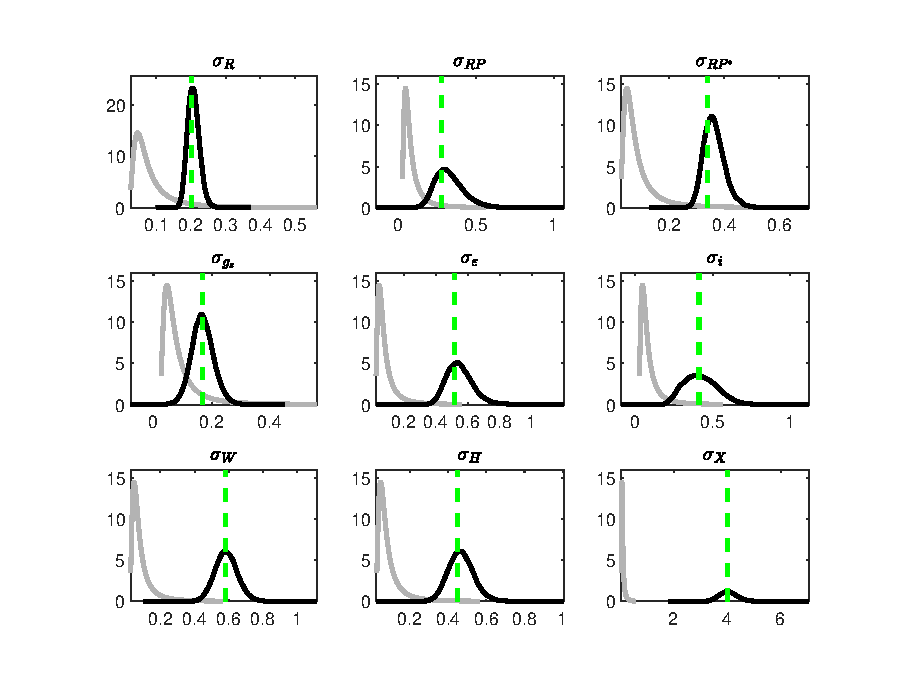
\includegraphics[width=10cm, trim =0 0 0.97cm 0]{SAFiscal_PriorsAndPosteriors1.eps} & 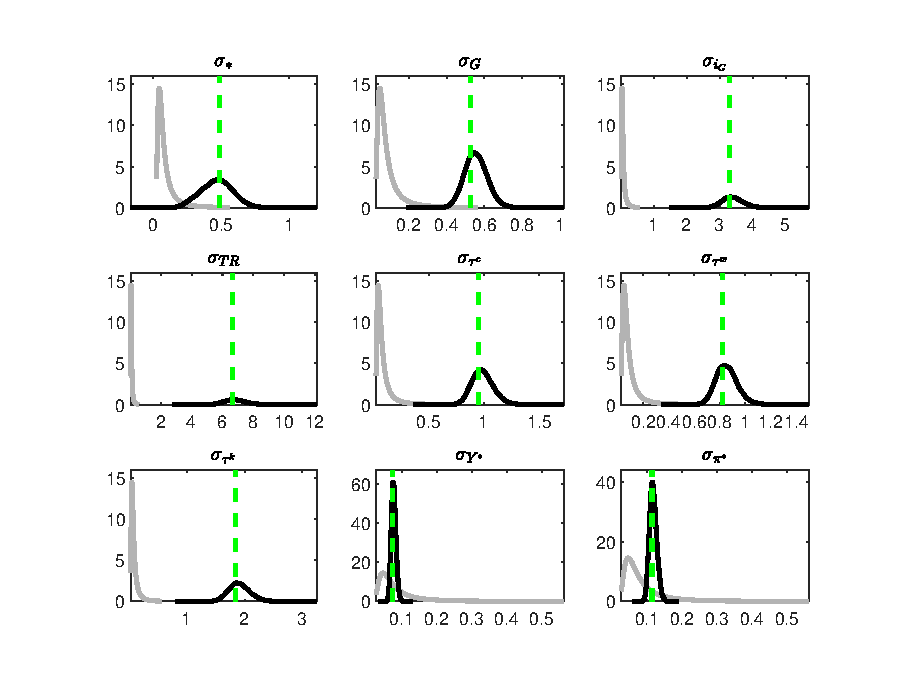
\includegraphics[width=10cm, trim =0.97cm 0 0 0]{SAFiscal_PriorsAndPosteriors2.eps}\\
	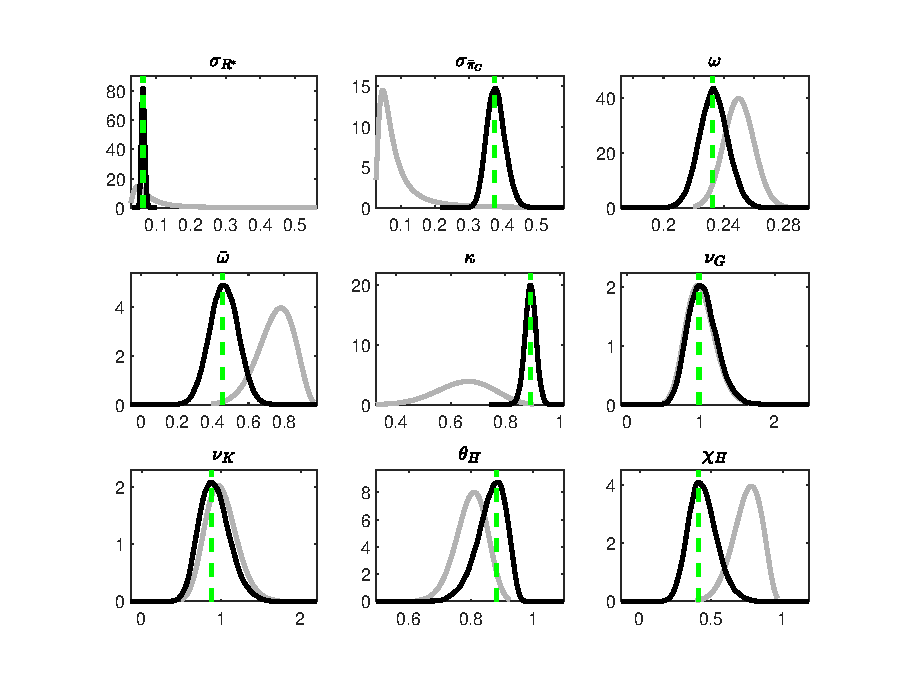
\includegraphics[width=10cm, trim =0 0 0.97cm 0]{SAFiscal_PriorsAndPosteriors3.eps} & 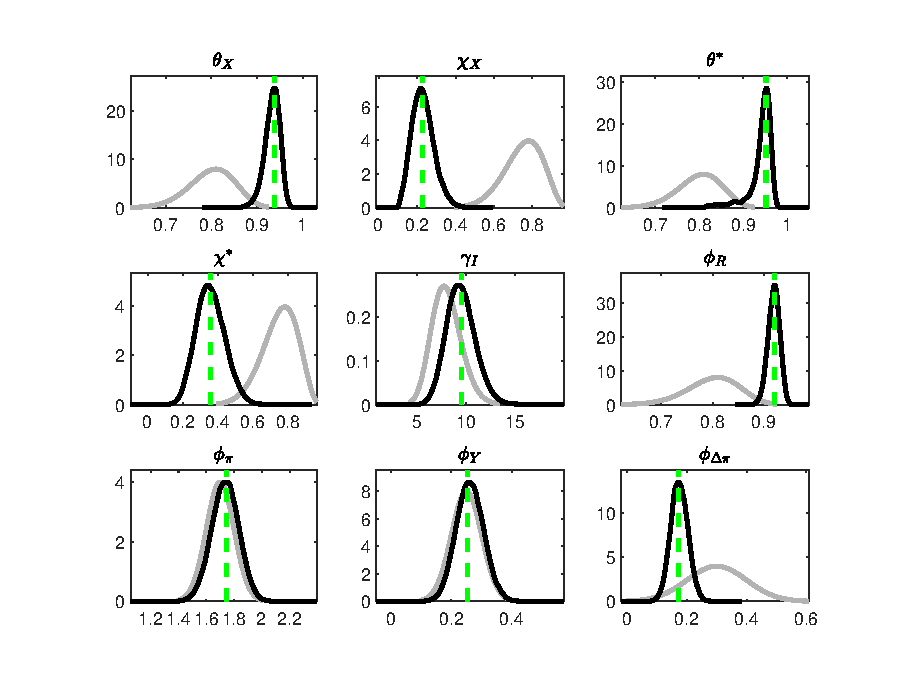
\includegraphics[width=10cm, trim =0.97cm 0 0 0]{SAFiscal_PriorsAndPosteriors4.eps}\\
	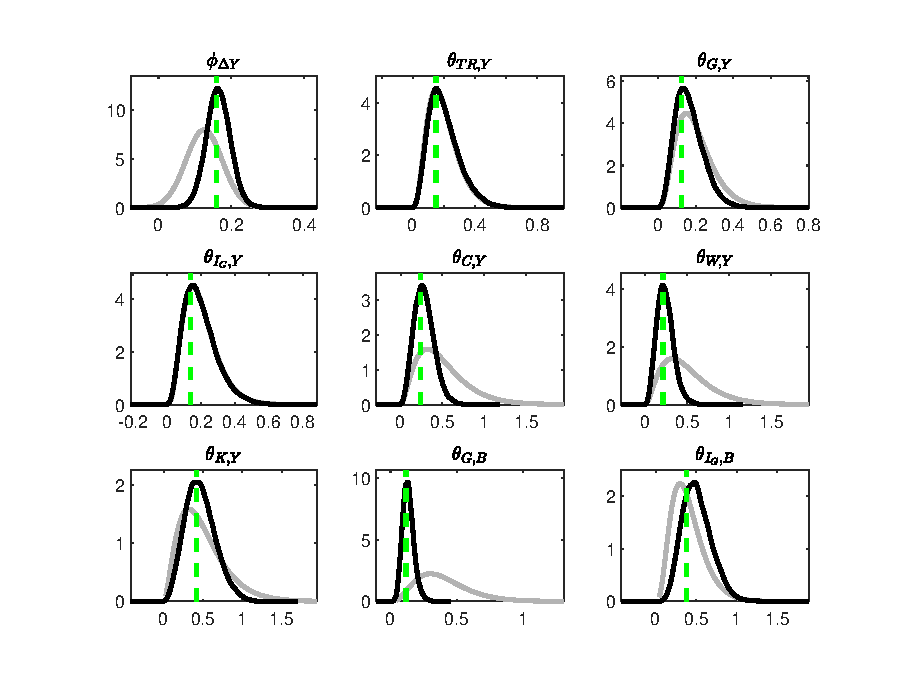
\includegraphics[width=10cm, trim =0 0 0.97cm 0]{SAFiscal_PriorsAndPosteriors5.eps} & 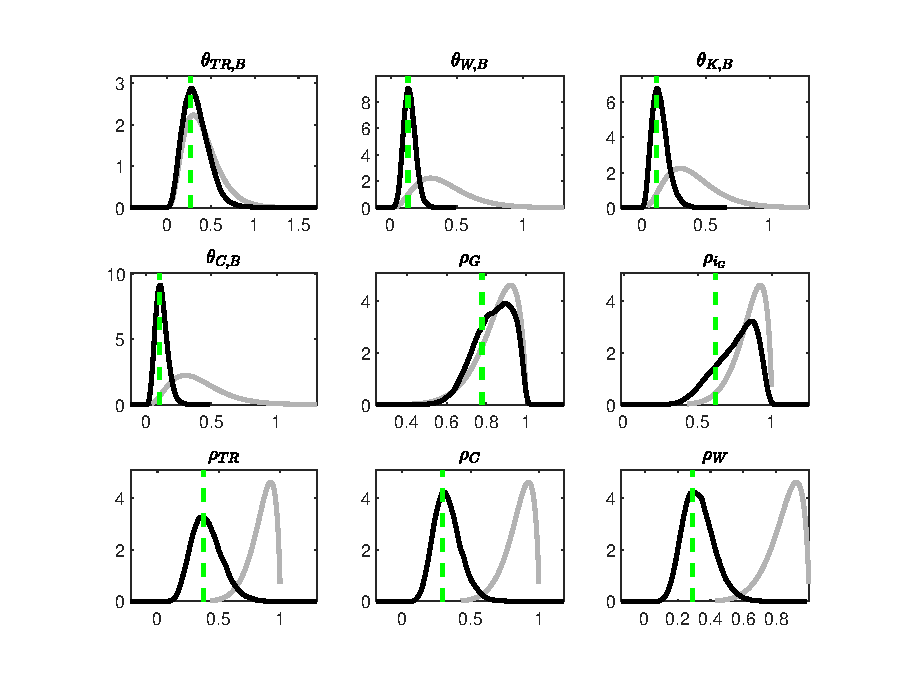
\includegraphics[width=10cm, trim =0.97cm 0 0 0]{SAFiscal_PriorsAndPosteriors6.eps}\\
\end{tabular}
}
\end{minipage}

\begin{minipage}{\linewidth}
	\captionof*{figure}{Figure C.1 (cont.): Prior and posterior densities}
	\makebox[\linewidth]{
		\begin{tabular}{p{10cm} p{10cm}}
			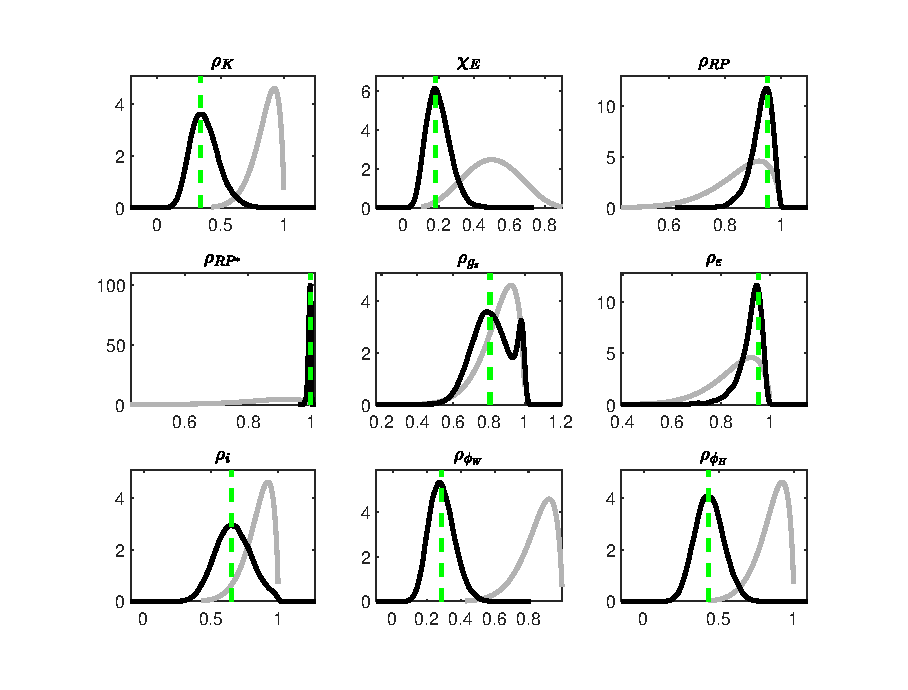
\includegraphics[width=10cm, trim =0 0 0.97cm 0]{SAFiscal_PriorsAndPosteriors7.eps} & 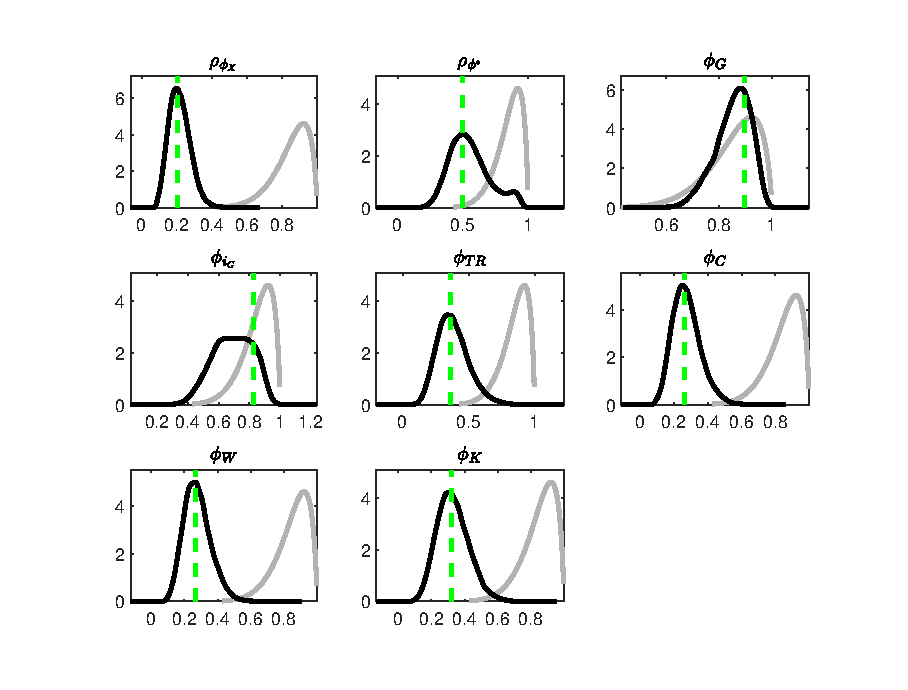
\includegraphics[width=10cm, trim =0.97cm 0 0 0]{SAFiscal_PriorsAndPosteriors8.eps}\\
			\label{fig_post_dens}
		\end{tabular}
	}
\end{minipage}

\begin{minipage}{\linewidth}
	\captionof{figure}{{Identification patterns at posterior mean (lowest singular value)}}
	\makebox[\linewidth]{
		\begin{tabular}{p{19cm}}
			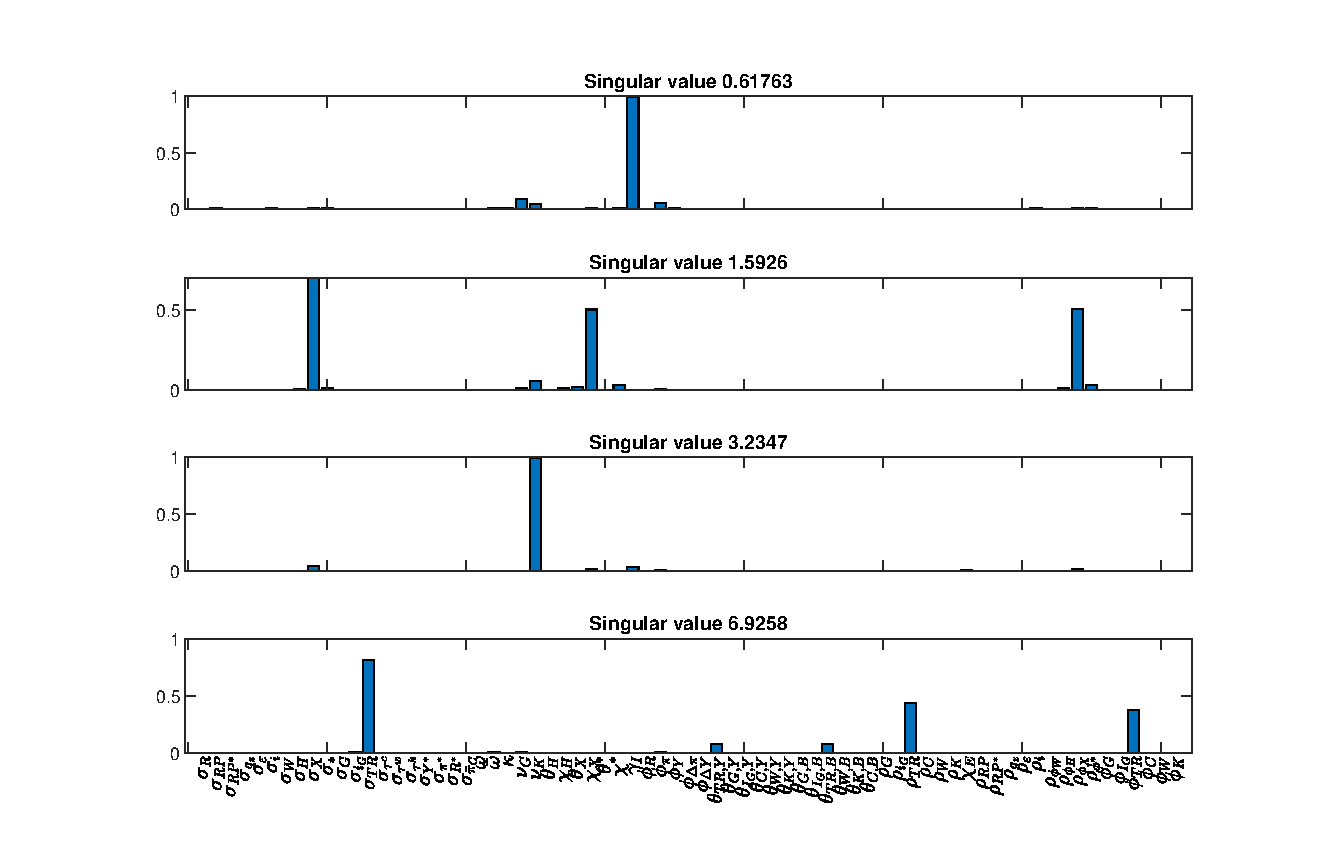
\includegraphics[width=19cm, trim =1cm 0 0 0.5cm]{SAFiscal_ident_pattern_posterior_mode_1.eps}\\
		\end{tabular}
		\label{fig_ident_pattern}
	}
\end{minipage}


\newpage
\begin{minipage}{\linewidth}
	\captionof{figure}{Identification strength at posterior mean}
	\makebox[\linewidth]{
		\begin{tabular}{p{22cm}}
			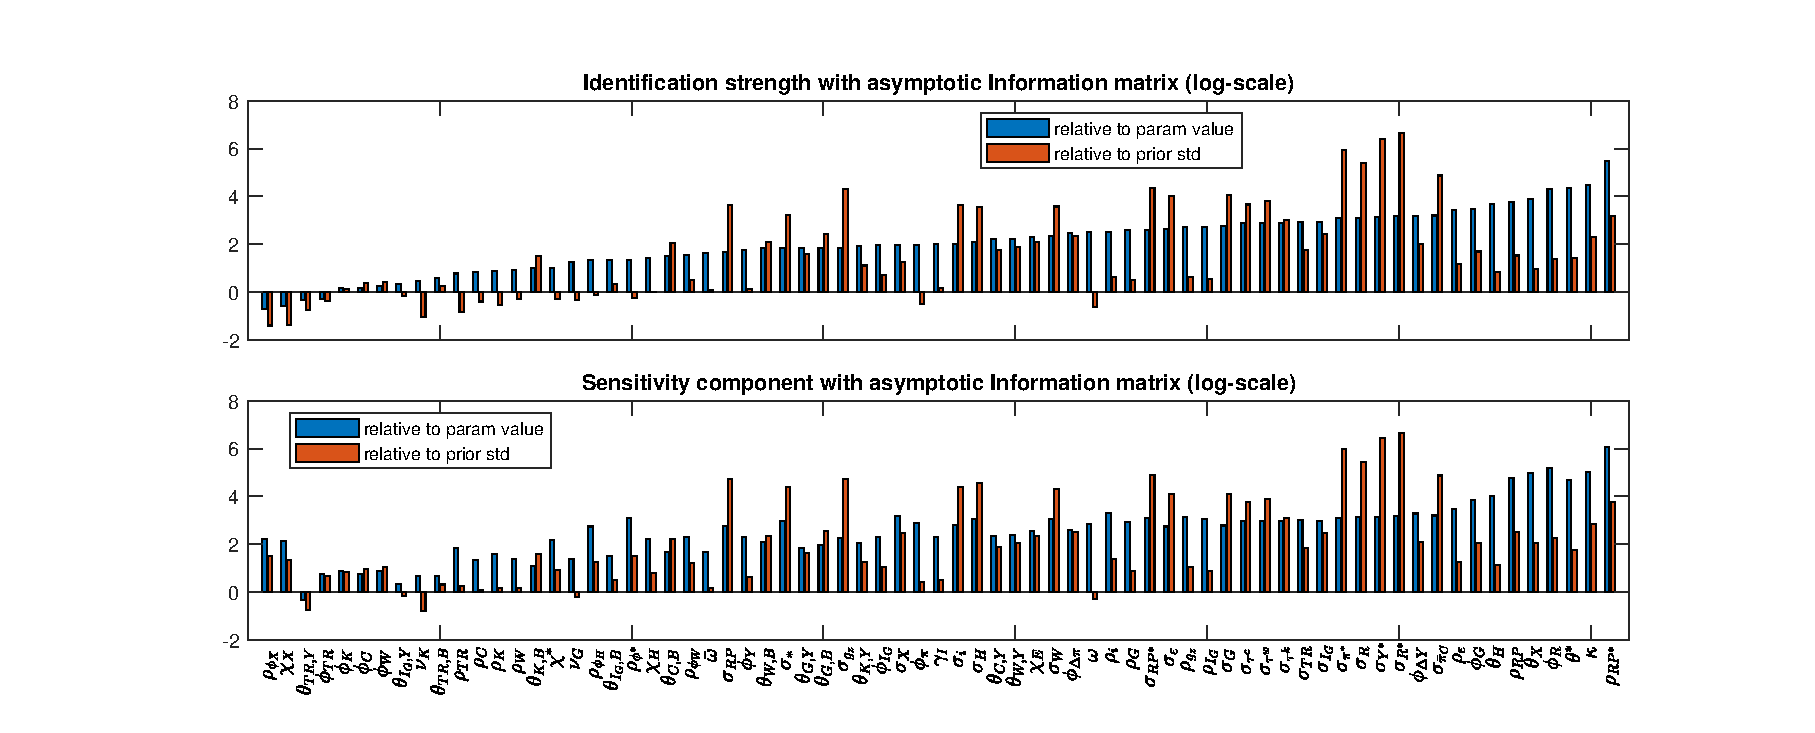
\includegraphics[width=22cm, trim =1cm 0 0 0]{SAFiscal_ident_strength_posterior_mode.eps}\\
		\end{tabular}
		\label{fig_ident}
	}
\end{minipage}

\vspace{1.2cm}
\begin{minipage}{\linewidth}
	\captionof{figure}{Sensitivity analysis at posterior mean}
	\makebox[\linewidth]{
		\begin{tabular}{p{22cm}}
			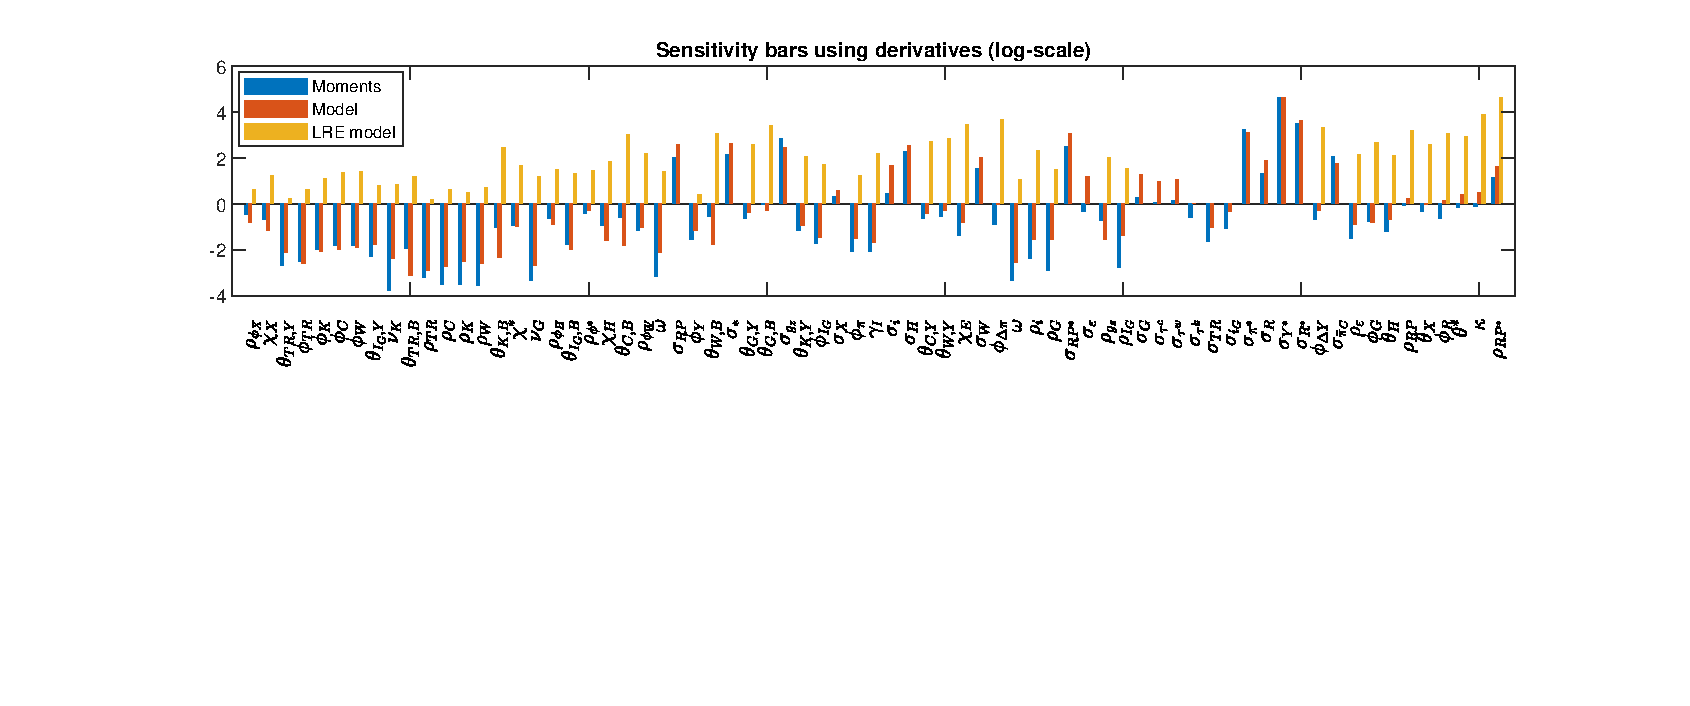
\includegraphics[width=22cm, trim =1cm 2cm 0 0.5cm]{SAFiscal_sensitivity_posterior_mode.eps}\\
		\end{tabular}
		\label{fig_sens}
	}
\end{minipage}

\newpage
\begin{minipage}{\linewidth}
	\captionof{figure}{Log-posterior likelihood functions and log-likelihood kernels}
	\makebox[\linewidth]{
		\begin{tabular}{p{9cm} p{9cm}}
			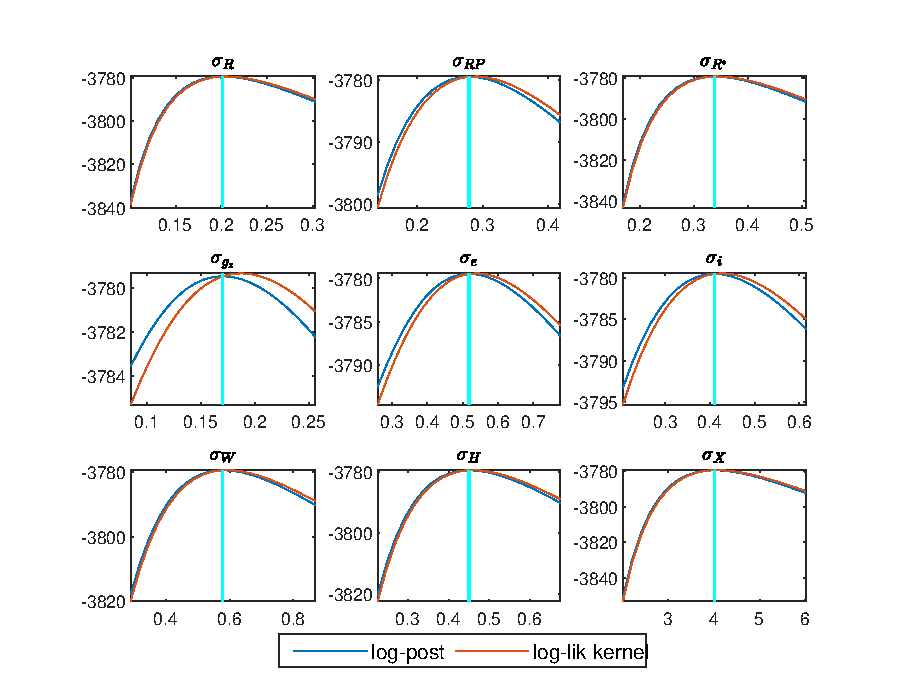
\includegraphics[width=9cm, trim =0 0 0.97cm 0]{SAFiscal_CheckPlots1.eps} & 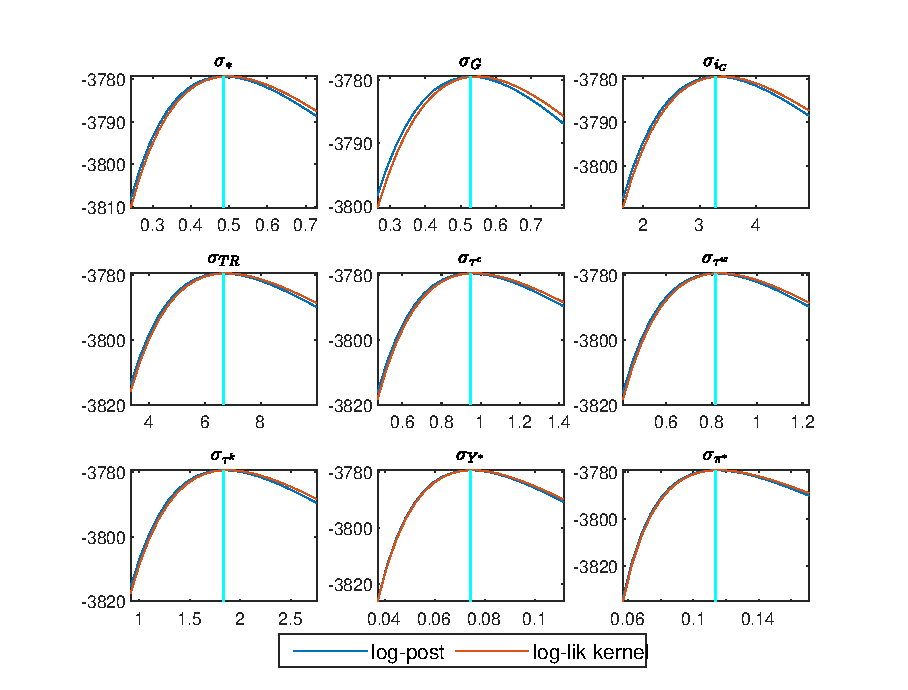
\includegraphics[width=9cm, trim =0.97cm 0 0 0]{SAFiscal_CheckPlots2.eps}\\
			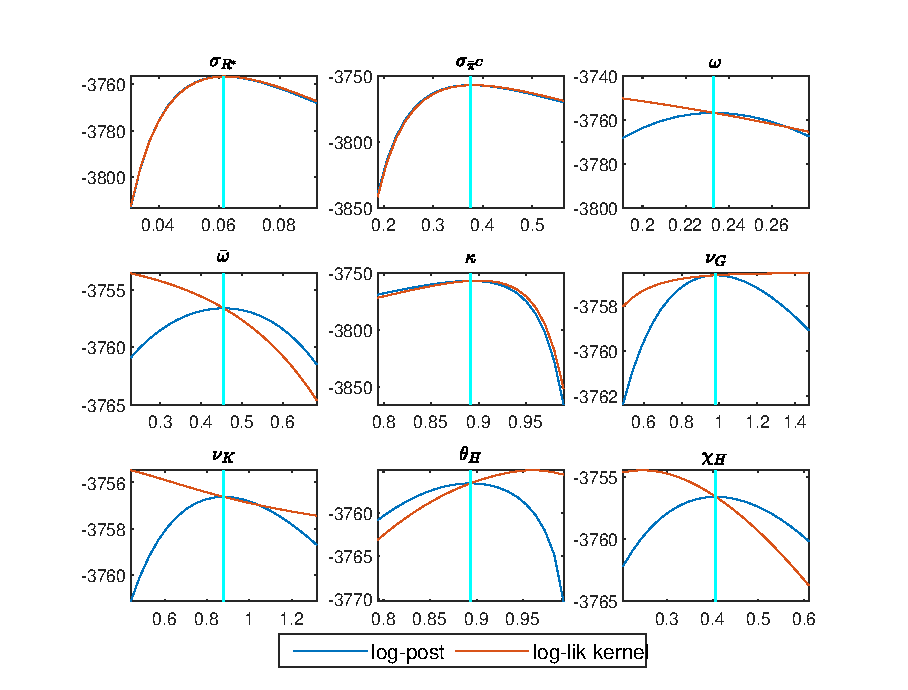
\includegraphics[width=9cm, trim =0 0 0.97cm 0]{SAFiscal_CheckPlots3.eps} & 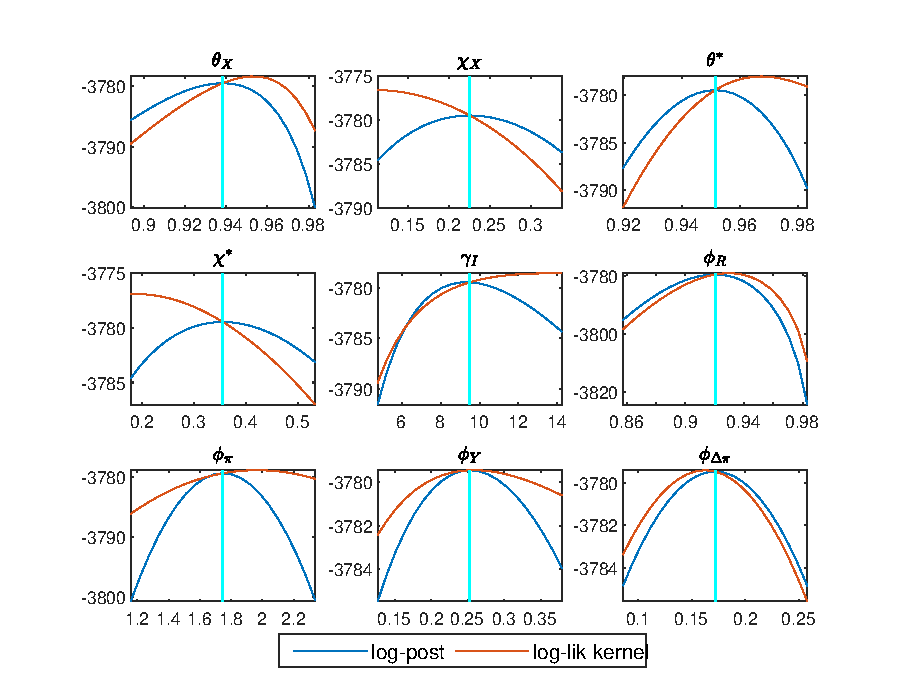
\includegraphics[width=9cm, trim =0.97cm 0 0 0]{SAFiscal_CheckPlots4.eps}\\
			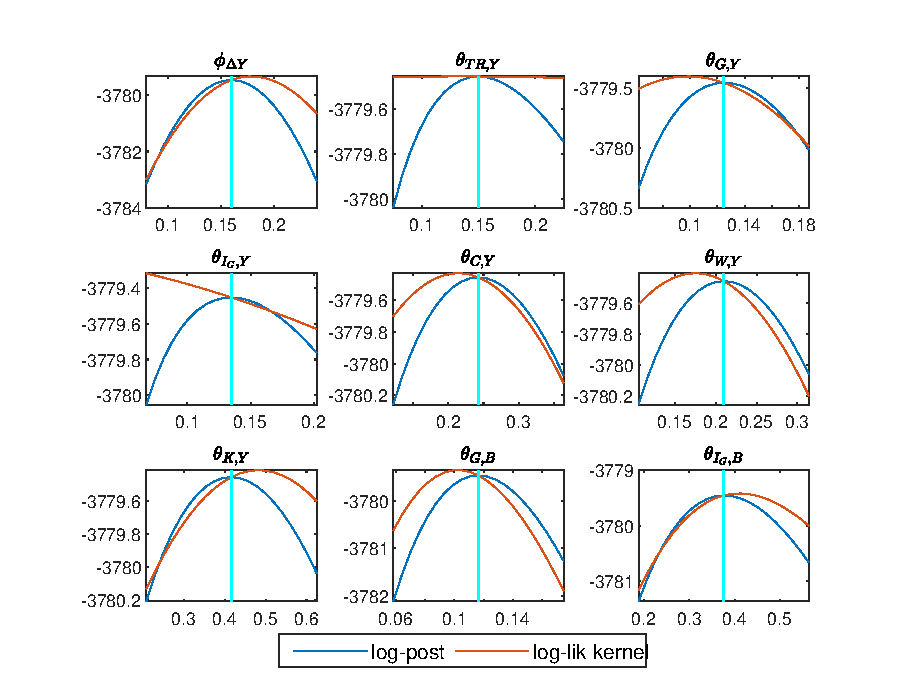
\includegraphics[width=9cm, trim =0 0 0.97cm 0]{SAFiscal_CheckPlots5.eps} & 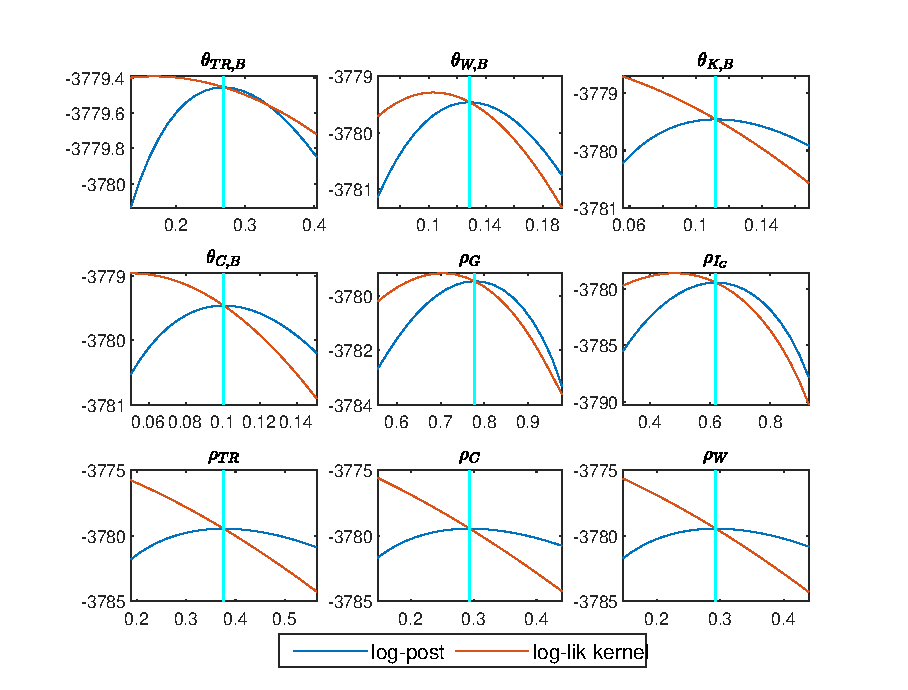
\includegraphics[width=9cm, trim =0.97cm 0 0 0]{SAFiscal_CheckPlots6.eps}\\
			\multicolumn{2}{c}{\footnotesize \textit{Note:} If the estimated mode is
				the local mode, it should be at the maximum of the posterior likelihood.}\\
			\label{fig_check_plot}
		\end{tabular}
	}
\end{minipage}

\newpage
\begin{minipage}{\linewidth}
	\captionof*{figure}{Figure C.5 (cont.): Log-posterior likelihood functions and log-likelihood kernels}
	\makebox[\linewidth]{
		\begin{tabular}{p{9cm} p{9cm}}
			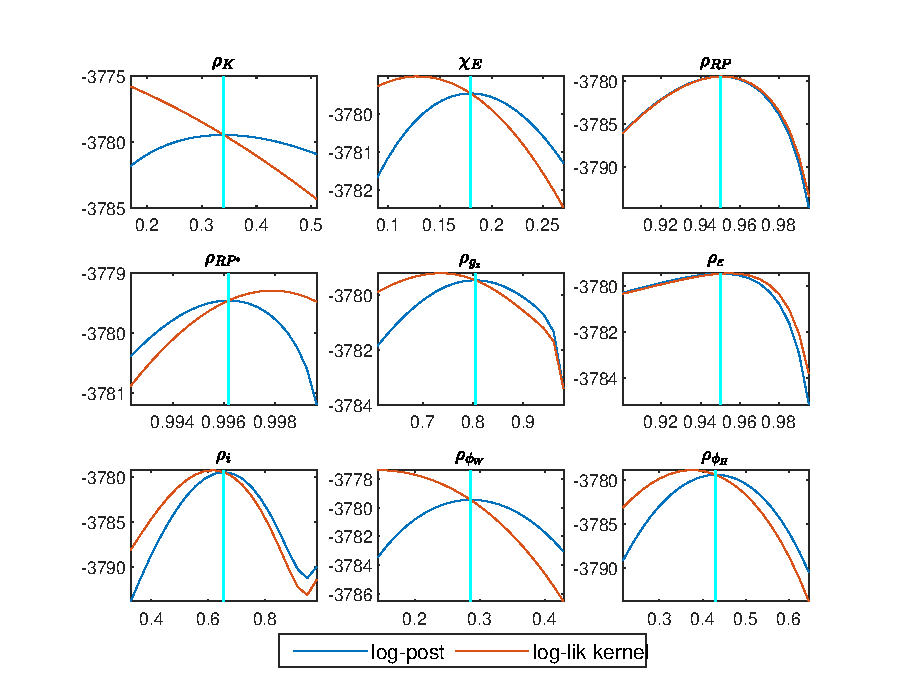
\includegraphics[width=9cm, trim =0 0 0.97cm 0]{SAFiscal_CheckPlots7.eps} & 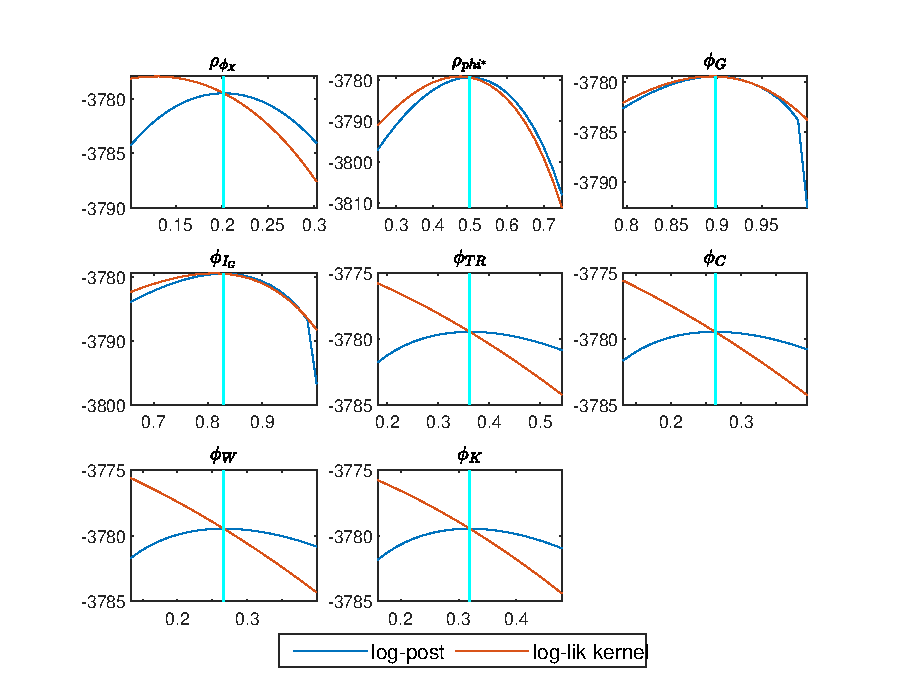
\includegraphics[width=9cm, trim =0.97cm 0 0 0]{SAFiscal_CheckPlots8.eps}\\
			\multicolumn{2}{c}{\footnotesize \textit{Note:} If the estimated mode is
				the local mode, it should be at the maximum of the posterior likelihood.}\\
		\end{tabular}
	}
\end{minipage}

\vspace{2cm}

\begin{minipage}{\linewidth}
	\captionof{figure}{Multivariate convergence diagnostic}
	\makebox[\linewidth]{
		\begin{tabular}{p{18cm}}
			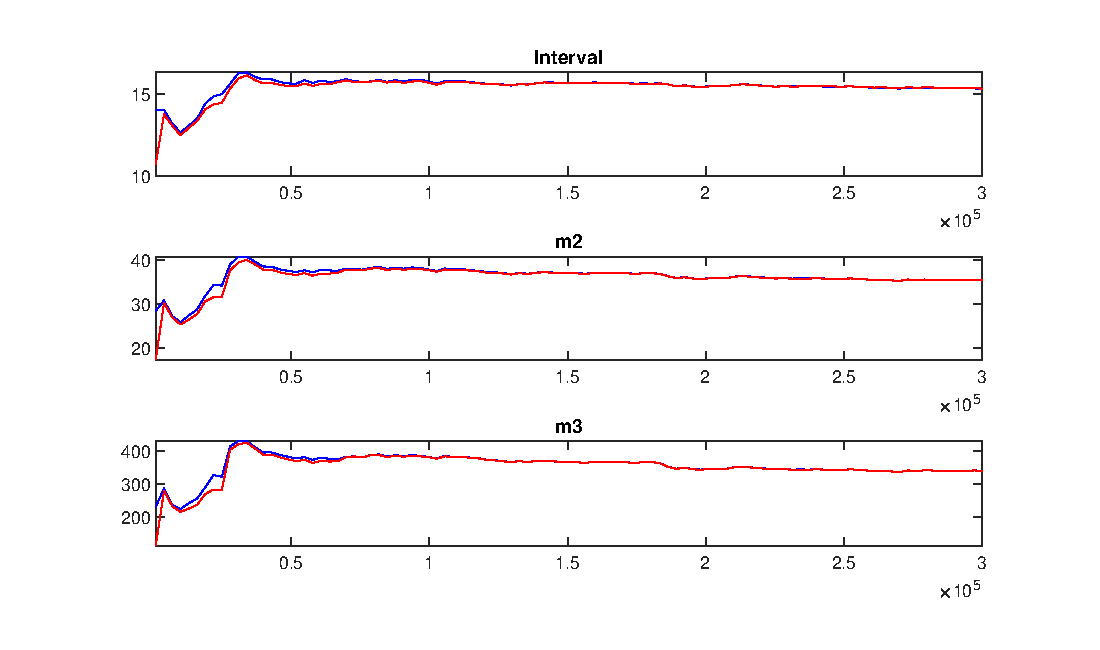
\includegraphics[width=18cm, trim =0 0 0 0.4cm]{SAFiscal_mdiag.eps}\\
		\end{tabular}
		\label{fig_mdiag}
	}
\end{minipage}


\newpage
\begin{minipage}{\linewidth}
	\captionof{figure}{Univariate convergence diagnostic}
	\makebox[\linewidth]{
		\begin{tabular}{p{9cm} p{9cm}}
			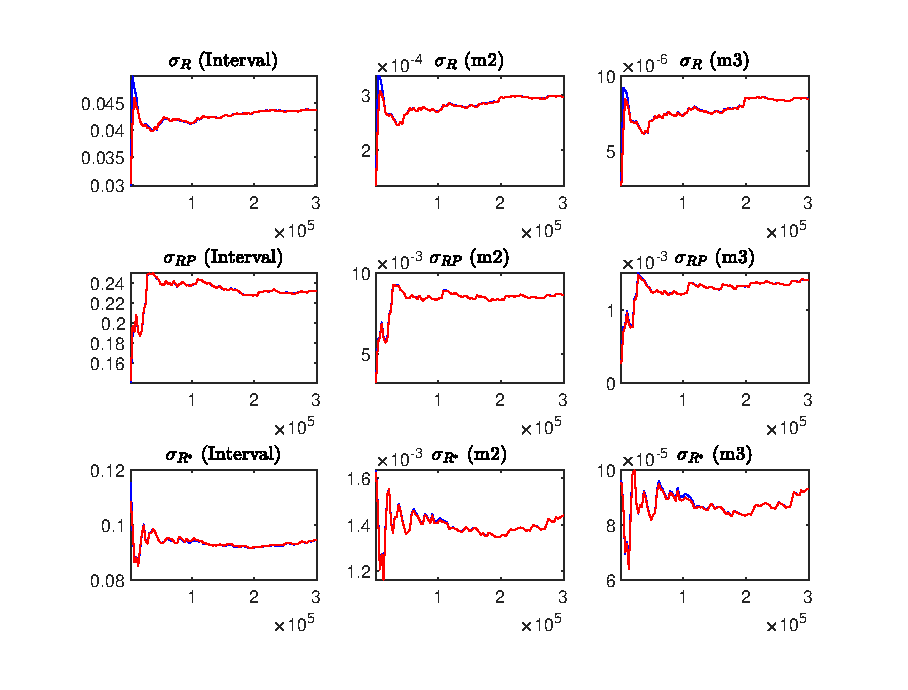
\includegraphics[width=9cm, trim =0 0 0.97cm 0]{SAFiscal_udiag1.eps} & 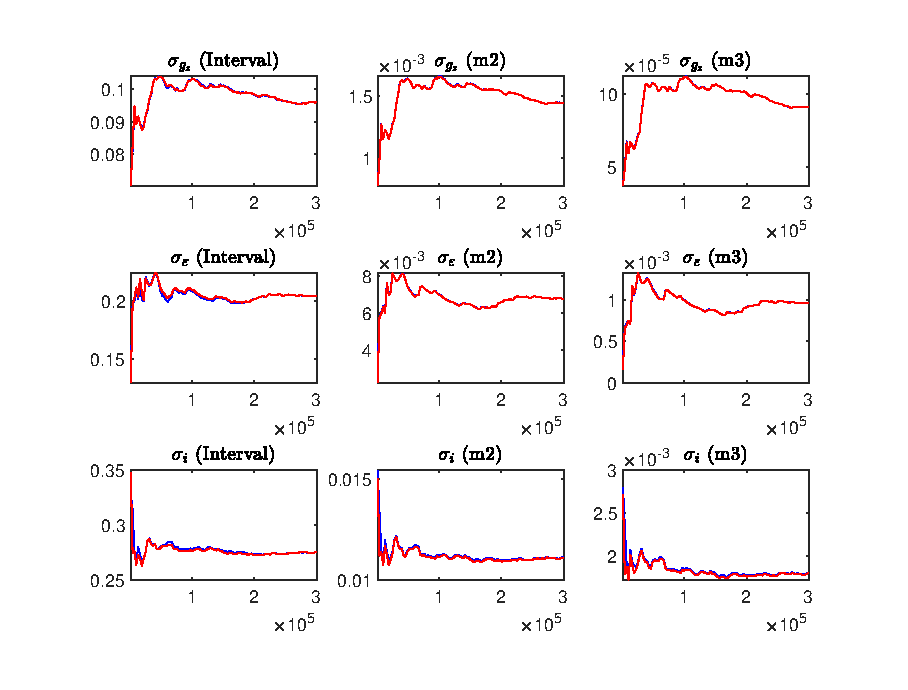
\includegraphics[width=9cm, trim =0.97cm 0 0 0]{SAFiscal_udiag2.eps}\\
			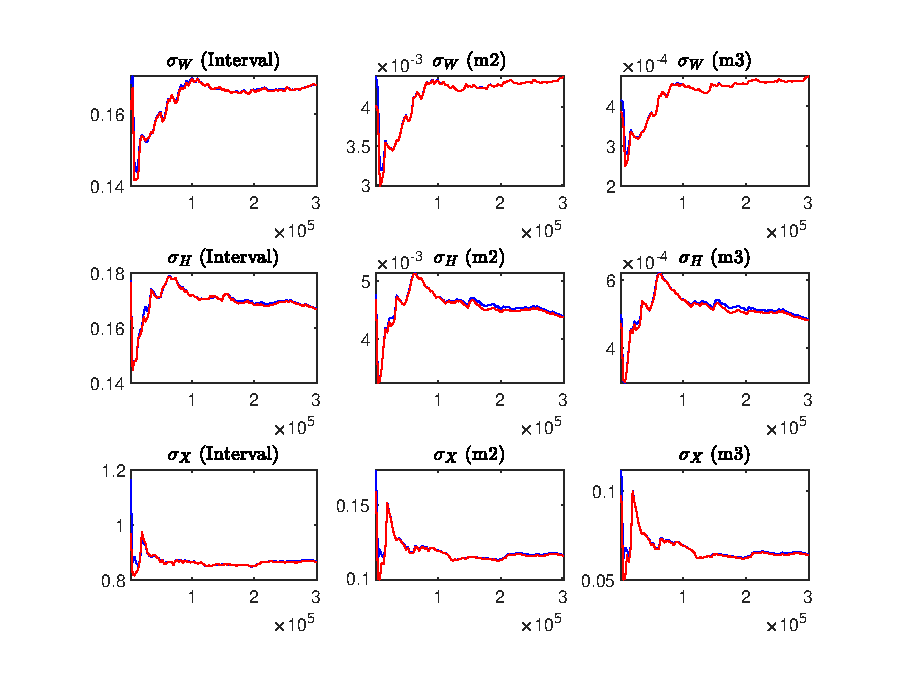
\includegraphics[width=9cm, trim =0 0 0.97cm 0]{SAFiscal_udiag3.eps} & 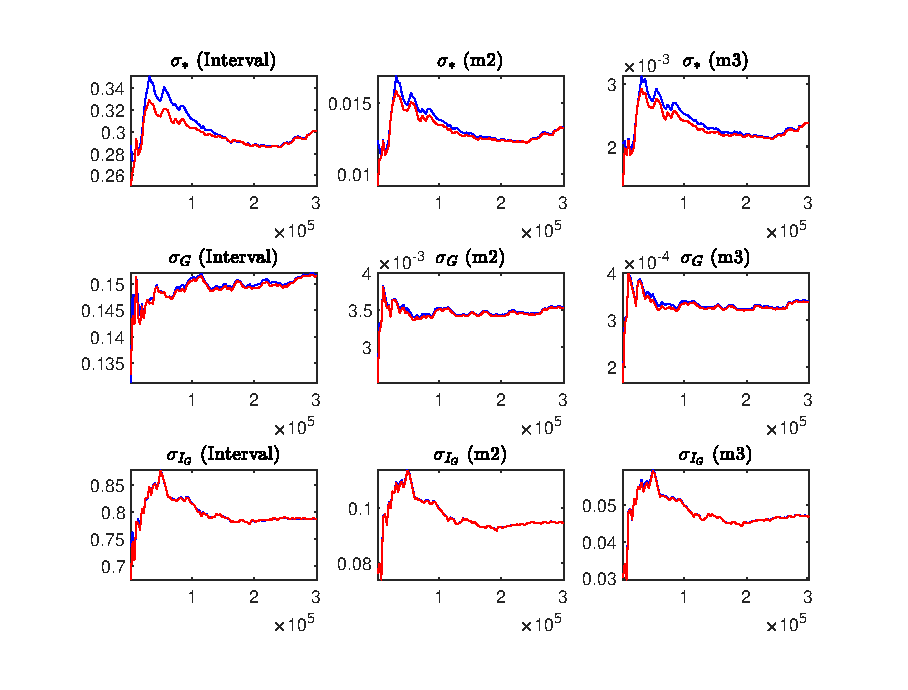
\includegraphics[width=9cm, trim =0.97cm 0 0 0]{SAFiscal_udiag4.eps}\\
			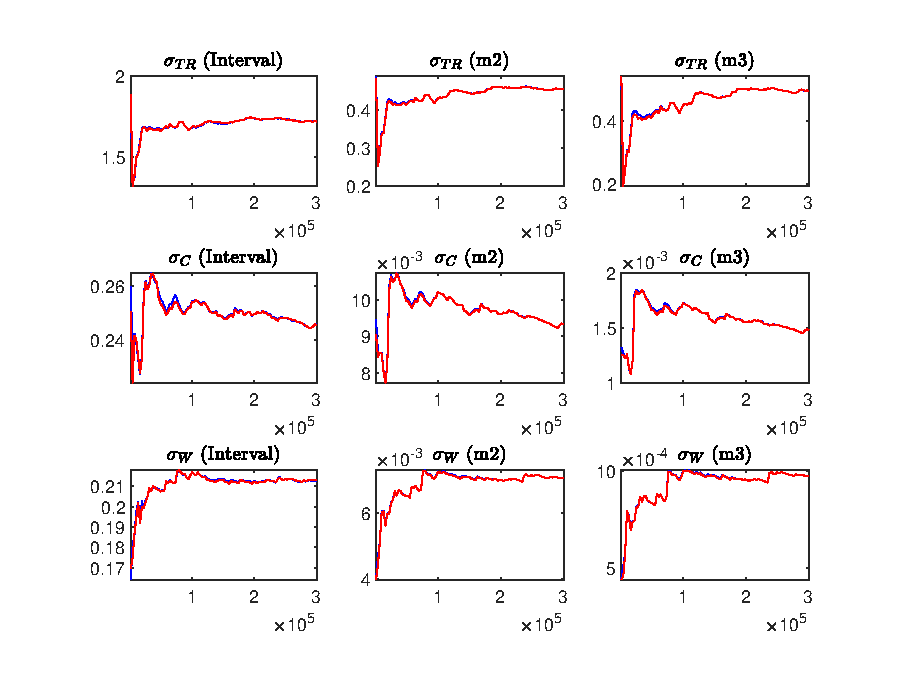
\includegraphics[width=9cm, trim =0 0 0.97cm 0]{SAFiscal_udiag5.eps} & 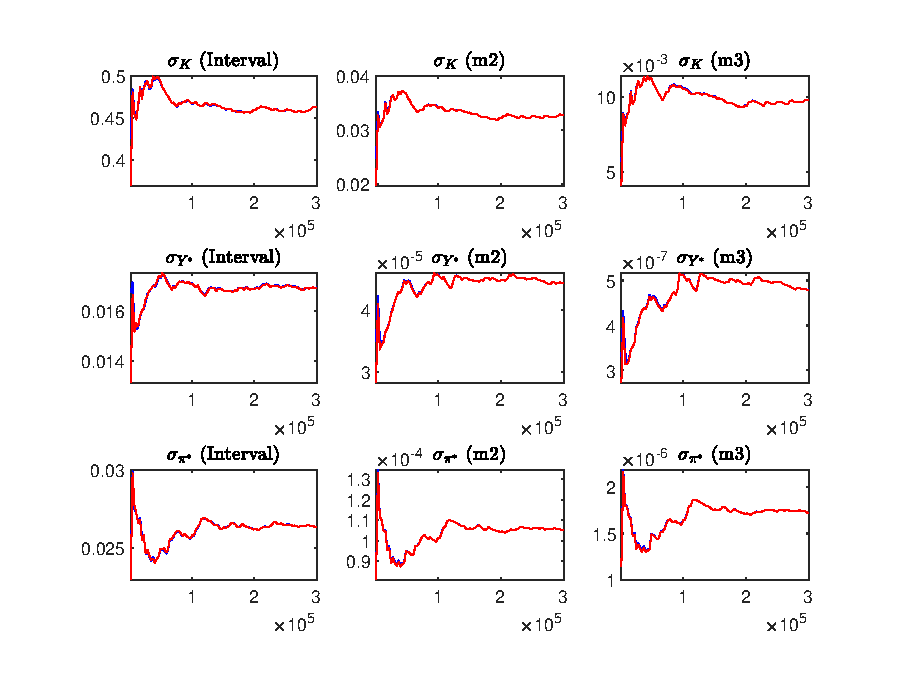
\includegraphics[width=9cm, trim =0.97cm 0 0 0]{SAFiscal_udiag6.eps}\\
			\label{fig_conv_plot}
		\end{tabular}
	}
\end{minipage}

\newpage
\begin{minipage}{\linewidth}
	\captionof*{figure}{Figure C.7 (cont.): Univariate convergence diagnostic}
	\makebox[\linewidth]{
		\begin{tabular}{p{9cm} p{9cm}}
			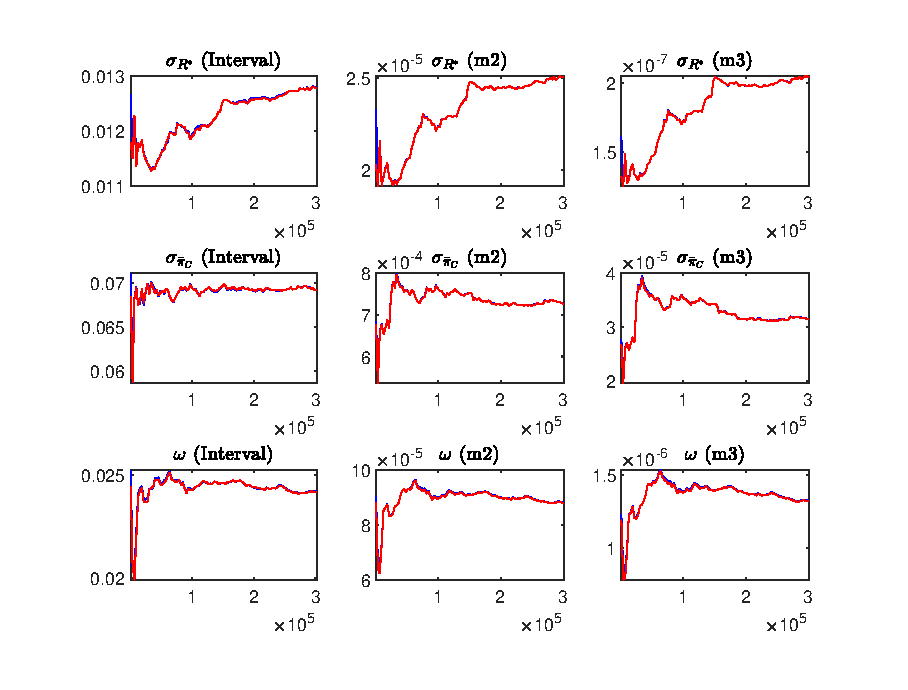
\includegraphics[width=9cm, trim =0 0 0.97cm 0]{SAFiscal_udiag7.eps} & 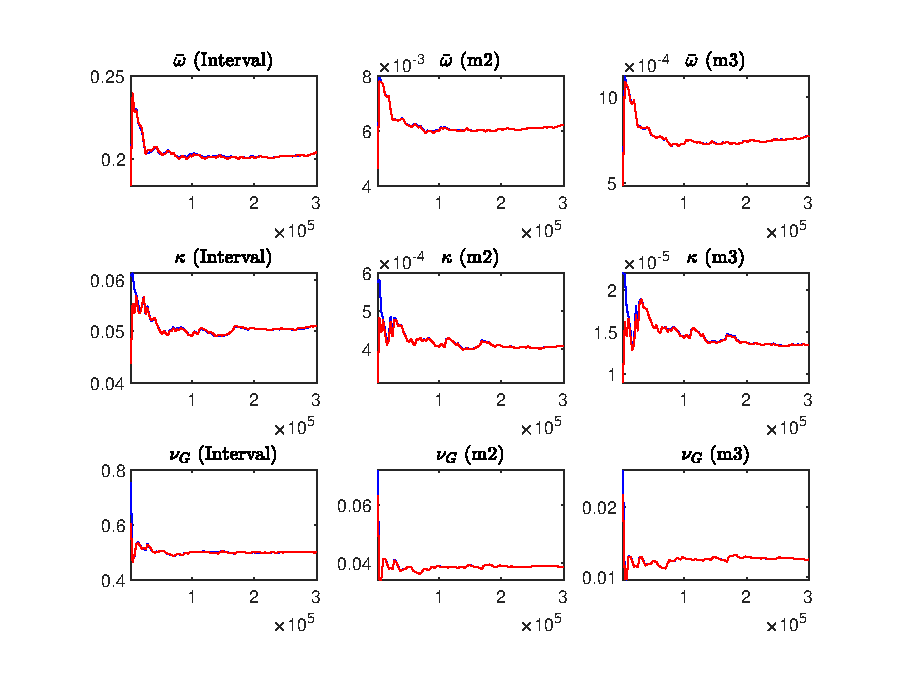
\includegraphics[width=9cm, trim =0.97cm 0 0 0]{SAFiscal_udiag8.eps}\\
			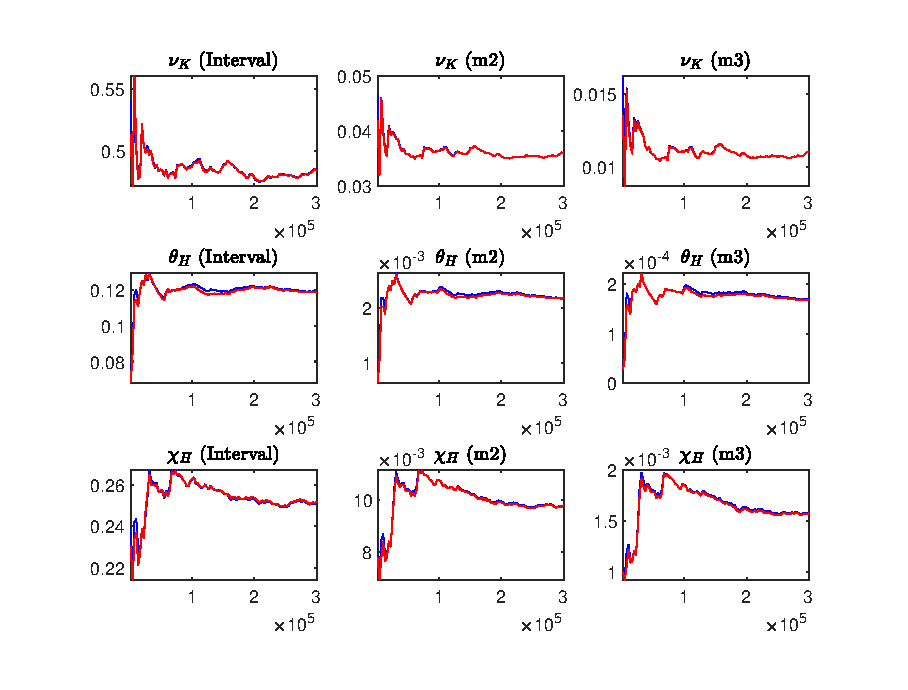
\includegraphics[width=9cm, trim =0 0 0.97cm 0]{SAFiscal_udiag9.eps} & 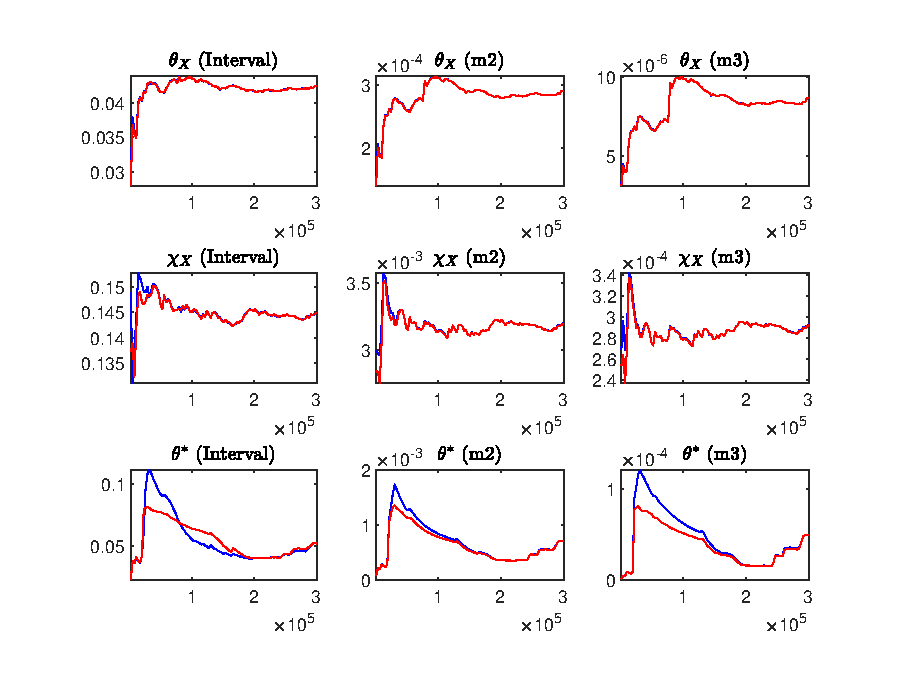
\includegraphics[width=9cm, trim =0.97cm 0 0 0]{SAFiscal_udiag10.eps}\\
			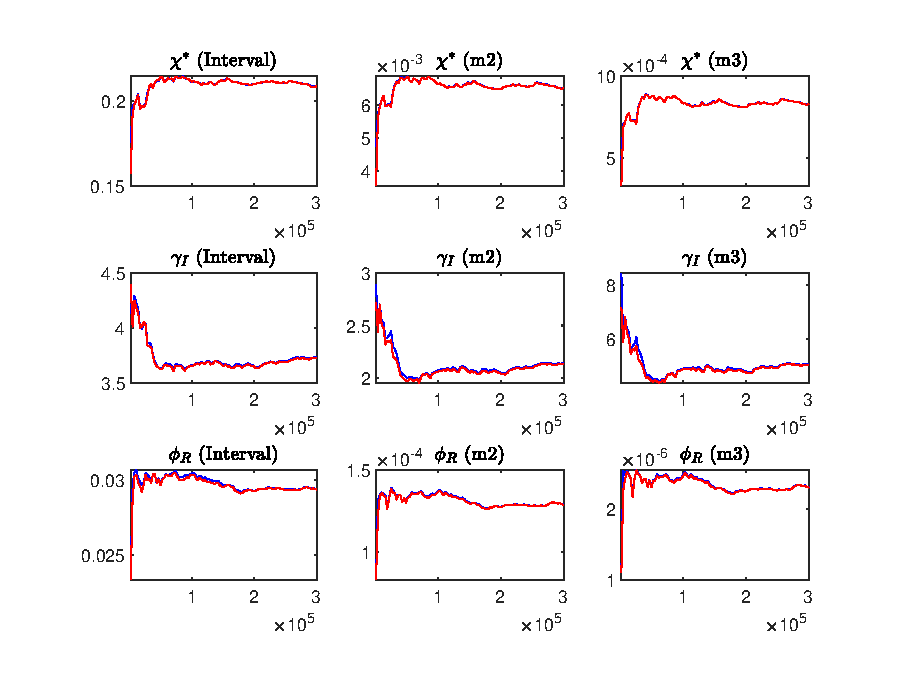
\includegraphics[width=9cm, trim =0 0 0.97cm 0]{SAFiscal_udiag11.eps} & 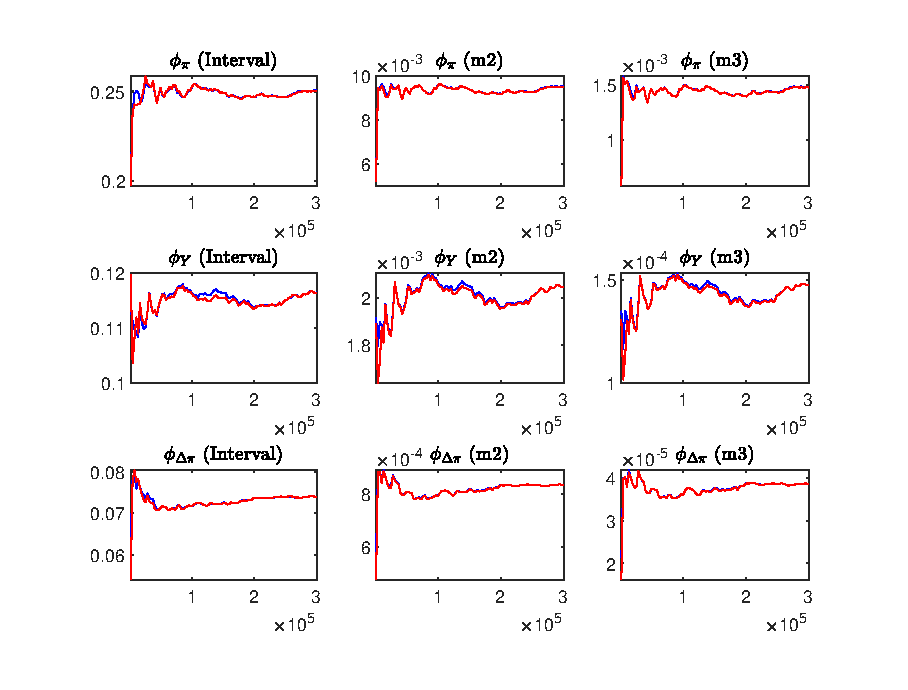
\includegraphics[width=9cm, trim =0.97cm 0 0 0]{SAFiscal_udiag12.eps}\\
		\end{tabular}
	}
\end{minipage}

\newpage
\begin{minipage}{\linewidth}
	\captionof*{figure}{Figure C.7 (cont.): Univariate convergence diagnostic}
	\makebox[\linewidth]{
		\begin{tabular}{p{9cm} p{9cm}}
			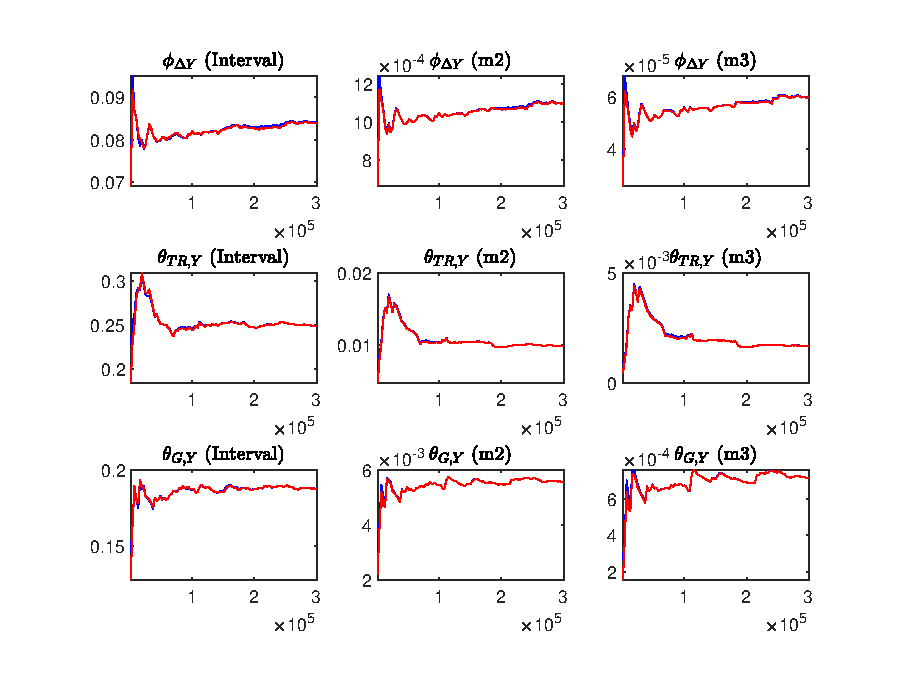
\includegraphics[width=9cm, trim =0 0 0.97cm 0]{SAFiscal_udiag13.eps} & 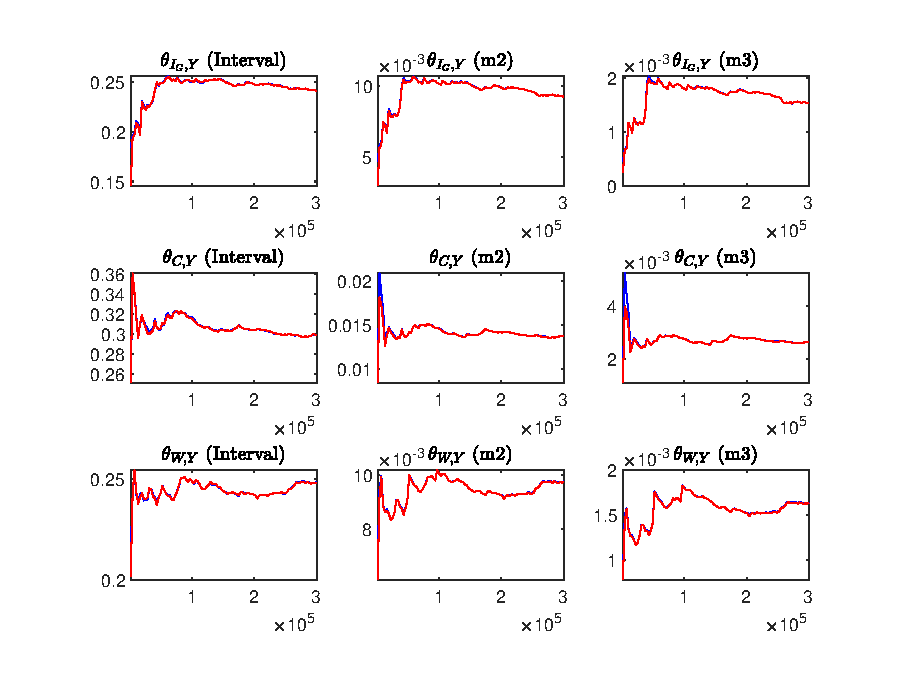
\includegraphics[width=9cm, trim =0.97cm 0 0 0]{SAFiscal_udiag14.eps}\\
			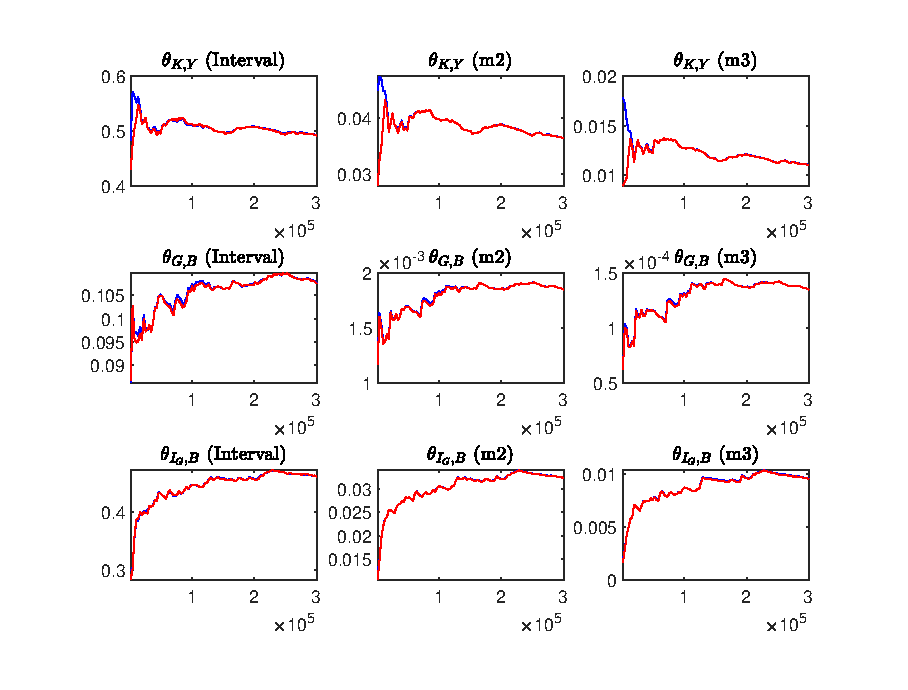
\includegraphics[width=9cm, trim =0 0 0.97cm 0]{SAFiscal_udiag15.eps} & 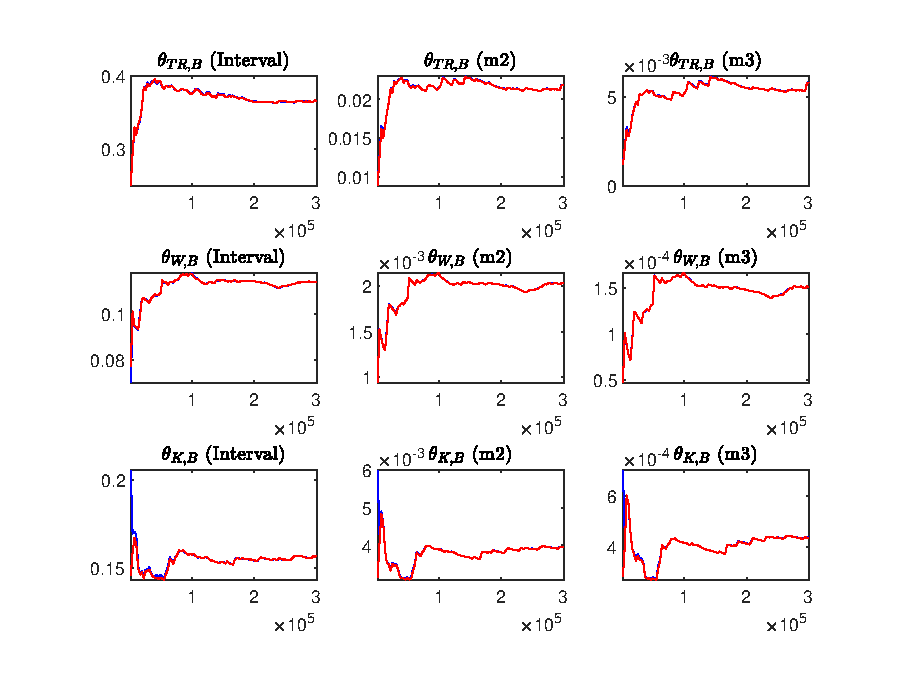
\includegraphics[width=9cm, trim =0.97cm 0 0 0]{SAFiscal_udiag16.eps}\\
			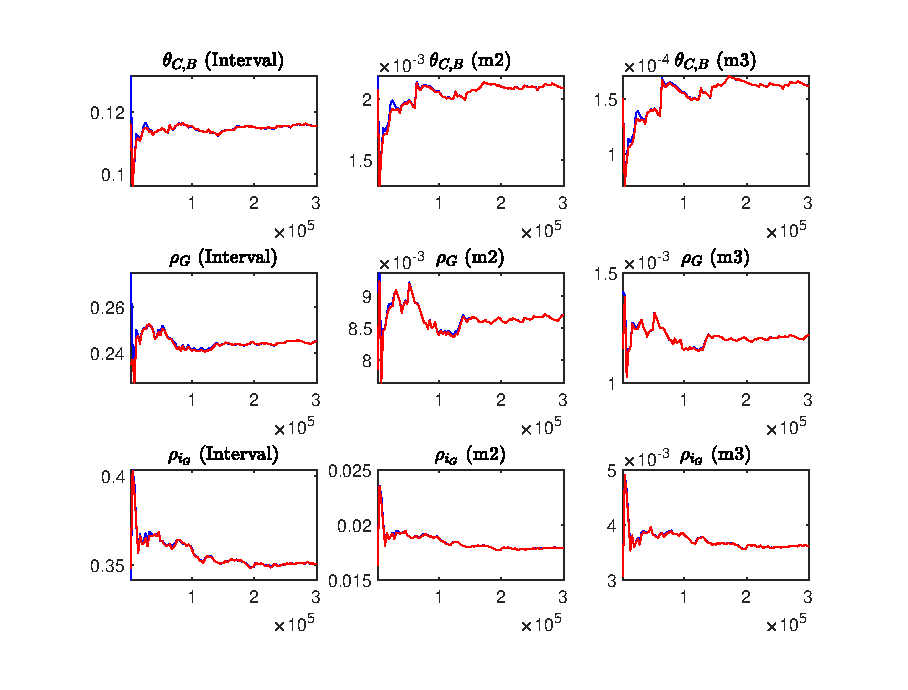
\includegraphics[width=9cm, trim =0 0 0.97cm 0]{SAFiscal_udiag17.eps} & \includegraphics[width=9cm, trim =0.97cm 0 0 0]{SAFiscal_udiag18.eps}\\
		\end{tabular}
	}
\end{minipage}

\newpage
\begin{minipage}{\linewidth}
	\captionof*{figure}{Figure C.7 (cont.): Univariate convergence diagnostic}
	\makebox[\linewidth]{
		\begin{tabular}{p{9cm} p{9cm}}
			\includegraphics[width=9cm, trim =0 0 0.97cm 0]{SAFiscal_udiag19.eps} & \includegraphics[width=9cm, trim =0.97cm 0 0 0]{SAFiscal_udiag20.eps}\\
			\includegraphics[width=9cm, trim =0 0 0.97cm 0]{SAFiscal_udiag21.eps} & \includegraphics[width=9cm, trim =0.97cm 0 0 0]{SAFiscal_udiag22.eps}\\
			\includegraphics[width=9cm, trim =0 0 0.97cm 0]{SAFiscal_udiag23.eps} & \raisebox{.85\height}{\includegraphics[width=9cm, trim =0 0 0 0]{SAFiscal_udiag24.eps}}\\
		\end{tabular}
	}
\end{minipage}

\newpage
\begin{table}[h]
	\small
	\centering
	\captionsetup{skip=6pt}
	\caption{Present-value multipliers: Gvt. spending and investment respond}
	\begin{tabular}{p{2cm} P{1.25cm} P{1.25cm} P{1.25cm} P{1.25cm} P{1.25cm}} 
		\toprule
		Variable& Q1 & Q4 & Q8 & Q20 & $\infty$ \\
		\hline
		\multicolumn{6}{l}{\textbf{Government consumption multiplier}} \\
		\hline
		$\frac{\Delta Y}{\Delta G}$ &0.05&0.26&0.31&0.31&0.29\\
		$\frac{\Delta C}{\Delta G}$ &-0.80&-0.67&-0.56&-0.41&-0.39\\
		$\frac{\Delta I}{\Delta G}$ &-0.06&-0.08&-0.09&-0.10&-0.09\\
		\hline
		\multicolumn{6}{l}{\textbf{Government investment multiplier}} \\
		\hline
		$\frac{\Delta Y}{\Delta I_G}$ &0.59&0.67&0.64&0.59&0.58\\
		$\frac{\Delta C}{\Delta I_G}$ &-0.03&-0.03&-0.03&0.02&0.03\\
		$\frac{\Delta I}{\Delta I_G}$ &-0.05&-0.07&-0.08&-0.07&-0.06\\
		\hline
		\multicolumn{6}{l}{\textbf{Labour tax multiplier}} \\
		\hline
		$\frac{\Delta Y}{\Delta T^w}$ &-0.45&-0.39&-0.27&-0.11&-0.09\\
		$\frac{\Delta C}{\Delta T^w}$ &-0.63&-0.82&-1.02&-1.19&-1.19\\
		$\frac{\Delta I}{\Delta T^w}$ &-0.01&-0.05&-0.11&-0.17&-0.17\\
		\hline
		\multicolumn{6}{l}{\textbf{Capital tax multiplier}} \\
		\hline
		$\frac{\Delta Y}{\Delta T^k}$ &-0.19&-0.14&0.03&0.27&0.29\\
		$\frac{\Delta C}{\Delta T^k}$ &-0.04&-0.35&-0.71&-1.07&-1.08\\
		$\frac{\Delta I}{\Delta T^k}$ &-0.04&-0.14&-0.26&-0.38&-0.38\\
		\hline
		\multicolumn{6}{l}{\textbf{Consumption tax multiplier}} \\
		\hline
		$\frac{\Delta Y}{\Delta T^c}$ &-0.23&-0.22&-0.09&0.10&0.12\\
		$\frac{\Delta C}{\Delta T^c}$ &-0.20&-0.58&-0.91&-1.17&-1.17\\
		$\frac{\Delta I}{\Delta T^c}$ &-0.01&-0.07&-0.14&-0.23&-0.23\\
		\toprule
		\multicolumn{6}{l}{\footnotesize \textit{Source:} Author's calculations.}\\
	\end{tabular}
	\label{pv_spend_tools}
\end{table}

\newpage
\begin{table}[h!]
	\small
	\centering
	\captionsetup{skip=6pt}
	\caption{Present-value multipliers: Taxes respond}
	\begin{tabular}{p{2cm} P{1.25cm} P{1.25cm} P{1.25cm} P{1.25cm} P{1.25cm}} 
		\toprule
		Variable& Q1 & Q4 & Q8 & Q20 & $\infty$ \\
		\hline
		\multicolumn{6}{l}{\textbf{Government consumption multiplier}} \\
		\hline
		$\frac{\Delta Y}{\Delta G}$ &-0.23&0.08&0.14&0.17&0.16\\
		$\frac{\Delta C}{\Delta G}$ &-0.87&-0.76&-0.70&-0.63&-0.62\\
		$\frac{\Delta I}{\Delta G}$ &-0.09&-0.12&-0.14&-0.17&-0.16\\
		\hline
		\multicolumn{6}{l}{\textbf{Government investment multiplier}} \\
		\hline
		$\frac{\Delta Y}{\Delta I_G}$ &0.48&0.56&0.52&0.48&0.48\\
		$\frac{\Delta C}{\Delta I_G}$ &-0.06&-0.11&-0.17&-0.23&-0.23\\
		$\frac{\Delta I}{\Delta I_G}$ &-0.06&-0.09&-0.12&-0.14&-0.13\\
		\hline
		\multicolumn{6}{l}{\textbf{Labour tax multiplier}} \\
		\hline
		$\frac{\Delta Y}{\Delta T^w}$ &-0.35&-0.33&-0.32&-0.30&-0.30\\
		$\frac{\Delta C}{\Delta T^w}$ &-0.60&-0.58&-0.56&-0.54&-0.53\\
		$\frac{\Delta I}{\Delta T^w}$ &0.01&0.03&0.05&0.07&0.07\\
		\hline
		\multicolumn{6}{l}{\textbf{Capital tax multiplier}} \\
		\hline
		$\frac{\Delta Y}{\Delta T^k}$ &-0.04&0.05&0.13&0.20&0.21\\
		$\frac{\Delta C}{\Delta T^k}$ &-0.02&0.20&0.38&0.53&0.53\\
		$\frac{\Delta I}{\Delta T^k}$ &-0.02&-0.05&-0.08&-0.12&-0.13\\
		\hline
		\multicolumn{6}{l}{\textbf{Consumption tax multiplier}} \\
		\hline
		$\frac{\Delta Y}{\Delta T^c}$ &-0.10&-0.10&-0.08&-0.06&-0.05\\
		$\frac{\Delta C}{\Delta T^c}$ &-0.17&-0.19&-0.18&-0.16&-0.15\\
		$\frac{\Delta I}{\Delta T^c}$ &0.01&0.03&0.05&0.07&0.07\\
		\toprule
		\multicolumn{6}{l}{\footnotesize \textit{Source:} Author's calculations.}\\
	\end{tabular}
	\label{pv_tax_tools}
\end{table}

	
\end{document}
